\documentclass{sig-alternate-10pt}
\usepackage{amsfonts,xspace}
\usepackage{url}
\usepackage{epsfig}
\usepackage{graphicx}
\usepackage{subfigure}
\usepackage{ifpdf}
\usepackage{epstopdf}
\usepackage[usenames,dvipsnames]{color}
%\newcommand{\tbd}[1]{}
\newcommand{\ie}{{\it i.e.}}
\newcommand{\eg}{{\it e.g.}}
\newcommand{\etc}{{\it etc.}}
\newcommand{\eat}[1]{}
\usepackage[english,plain]{fancyref}
\usepackage{times}
\usepackage{rotating}
\usepackage[labelformat=simple]{subfig}
\usepackage{multirow}

\newcommand{\mypara}[1]{\medskip\noindent{\bf {#1}:}~}
\newcommand{\chk}{$\checkmark$}
\newcommand{\dsh}{{\bf --}}
\newcommand{\til}{{\bf\large \textasciitilde}}
\newcommand{\tbd}[1]{[{\color{red}{\bf{TBD: #1}}}]}
\newcommand{\etal}{\emph{et~al.}}
\newcommand{\meddle}{{\emph{Meddle}}\xspace}
\newcommand{\meddleT}{{Meddle}\xspace}
\newcommand{\dsum}{\displaystyle\sum}
\newcounter{packednmbr}
\newcommand{\iphone}{iPhone\xspace}
\newcommand{\wifi}{Wi-Fi\xspace}
\newcommand{\postfigspace}{0em}
\newcommand{\figcapspace}{0em}


\newenvironment{packedenumerate}{\begin{list}{\thepackednmbr.}{\usecounter{packednmbr}\setlength{\itemsep}{0.2pt}\addtolength{\labelwidth}{-4pt}\setlength{\leftmargin}{\labelwidth}\setlength{\listparindent}{\parindent}\setlength{\parsep}{1pt}\setlength{\topsep}{0pt}}}{\end{list}}
\newenvironment{packeditemize}{\begin{list}{$\bullet$}{\setlength{\itemsep}{0.2pt}\addtolength{\labelwidth}{-4pt}\setlength{\leftmargin}{\labelwidth}\setlength{\listparindent}{\parindent}\setlength{\parsep}{1pt}\setlength{\topsep}{0pt}}}{\end{list}}
\newenvironment{packedtrivlist}{\begin{list}{\setlength{\itemsep}{0.2pt}\addtolength{\labelwidth}{-4pt}\setlength{\leftmargin}{\labelwidth}\setlength{\listparindent}{\parindent}\setlength{\parsep}{1pt}\setlength{\topsep}{0pt}}}{\end{list}}

\renewcommand{\fref}{\Fref}
\renewcommand\thesubfigure{~(\alph{subfigure})}

\title{Meddle: Transparency and Control for Mobile Network Traffic}

\numberofauthors{8}
\author{
\alignauthor
Ashwin Rao\\
\affaddr{Inria}
\alignauthor
Amy Tang\\
\affaddr{UC Berkeley}
\alignauthor        
Justine Sherry\\
\affaddr{UC Berkeley}
\and
\alignauthor
Arnaud Legout\\
\affaddr{Inria}
\alignauthor
Walid Dabbous\\
\affaddr{Inria}
\alignauthor 
Arvind Krishnamurthy\\
\affaddr{University of Washington}
\and
\alignauthor
David Choffnes\\
\affaddr{University of Washington}
}

\date{}
\begin{document}	
\maketitle

\subsection*{Abstract}

We present, Meddle, a platform that relies on traffic indirection to diagnose mobile Internet traffic.
Meddle is motivated by the absence of built-in support from ISPs and mobile OSes to freely monitor and control mobile Internet traffic; the restrictions imposed by mobile OSes and ISPs also make existing approaches impractical.
%Instrumenting mobile OSes, static and dynamic analysis of application binaries, or the privilege of working with ISPs---impractical. 
Meddle overcomes these hurdles by relying on the native support for traffic indirection by mobile OSes.
Specifically, Meddle proxies mobile Internet traffic through a software defined middleboxes configured for mobile traffic diagnosis. 
In this paper, we use Meddle to tests the limits of the network perspective of mobile Internet traffic offered by traffic indirection. 

We use this perspective to characterize and control the behavior of mobile applications and provide a first look at ISP interference on mobile Internet traffic. 
\tbd{We report on controlled experiments we conducted to analyze the network behavior of 100 most popular iOS and Android applications.}
\tbd{We also report on how ISP interfere with mobile HTTP Internet traffic.}








%%% Local Variables: 
%%% mode: latex
%%% TeX-master: "meddle-main"
%%% End: 


\section{Introduction}
\label{sec:introduction}

%what is the problem area you are working in and why is it important? It is important to set the larger context here. Why is the problem of interest and importance to the larger community?

Mobile systems consist of walled gardens inside gated communities, i.e., locked-down operating systems running on devices that interact over a closed and opaque mobile network. 
Despite a large collection of privacy, policy and performance issues in mobile networks~\cite{enck:taintdroid,hornyack:appfence,speedtest,pathak:eprof}, researchers are faced with few options to characterize and address them.

%What is the specific problem considered in this paper? This paragraph narrows down the topic area of the paper. In the first paragraph you have established general context and importance. Here you establish specific context and background.
%Cannot mention user participation and crowd sourcing here because we have not achieved it in this work . 
%What we have here is a platform with a potential for user participation and preliminary results. 

The key challenge is that mobile devices, their OSes, and ISPs provide no built-in service to monitor and control \emph{all network traffic}.
As a result, previous studies~\cite{vallina-rod:ads,gerber:passivespeed,chen:wifi,enck:taintdroid,wang:middleboxes,sommers:cellwifi} are constrained by at least one of the following: mobile OSes, access technology, device manufacturer, installed applications, and user behavior.
In this work, we are the first to present an approach that compromises none of these, an approach that can be used across carriers, mobile devices, apps, and access technologies.

\meddle redirects all Internet traffic through a software-defined middlebox for the purpose of analysis and interposition.
Specifically, \meddle builds on the native support for VPN tunnels by mobile OSes to tunnel all the Internet traffic regardless of the access technology used by the device. 

\tbd{tripwire stuff}


In this paper, we use \meddle to test the limits to which mobile Internet traffic can be diagnosed using traffic redirection.
The main contributions of this paper are as follows:
\begin{packedenumerate}
\item Platform for practical mobile diagnosis. Single server solution empowers users to install and configure them on home-gateways.
Researchers can deploy them for measurement studies. 
\item Controlled experiments using off-the-shelf Android and iOS devices. 
\item Controlled experiments to analyze ISP interference in US and France. 
\end{packedenumerate}

The remainder of this paper is structured as follows.

%%% Local Variables: 
%%% mode: latex
%%% TeX-master: "meddle-main"
%%% End: 



\section{Goals and Architecture}
In this section, we discuss the motivation for \meddle, describe our goals for the 
system and present an architecture to meet those goals.

\meddle is motivated by the fact that users and researchers currently 
have a limited view -- if any -- into how devices and apps generate network 
traffic. In addition, there are few mechanisms available for shaping, modifying 
or blocking this network traffic. 

This can be harmful to users, as apps may generate sufficient traffic
to cause overage charges on cell phone bills. Even when the volume of
traffic is small, a periodic network activity can quickly deplete
battery charge by preventing power management policy of the device to
correctly operate. Further, apps can use the network to leak personal
information or track users without consent.

Researchers  are in a similar bind. It is common 
to use testbeds or proprietary ISP datasets to reveal network usage 
and its impact on data quota, battery life and privacy. However, the 
coverage and representativeness of these results can by limited by 
the use of i) a single carrier's network, ii) a small testbed with 
a single, custom operating system and iii) a single access technology 
(cellular or WiFi). Once a problem with network traffic has been identified, 
addressing it can be challenging. OS developers are slow to 
adopt changes, app developers may be unwilling to modify their code 
and carriers often have no incentive to deploy new in-network 
functionality. 

%However, there is a large and dynamic set of 
%apps, devices and usage patterns that are not captured in the lab 
%environment. Assuming that such studies reveal pathological control network traffic is similarly limited, as 
%it may require changes to the operating system and to apps.  Even  Without visibility 
%into how apps and devices use the network in the wild, 
%To characterize mobile traffic and design new protocols and
%services that are better tailored to the mobile environment, we would like a
%framework that allows us to intercept and potentially modify traffic
%generated by mobile devices as they move with users, regardless of the
%device, OS or carrier. However, implementing this functionality is
%difficult on mobile devices because it requires warranty-voiding
%techniques such as jail breaking to access and manipulate traffic at
%the network layer~\cite{enck:taintdroid}. Even when using such an
%approach, carriers may manipulate traffic once it leaves the mobile
%device~\cite{wang:middleboxes}, thus rendering some research
%impractical. Last, some protocols and services should be implemented
%in the network instead of the device (e.g., prefetching and security
%filters) but researchers generally have no ability to deploy such
%solutions.

\subsection{System Goals}
The two primary goals for \meddle are 1) to provide comprehensive visibility into 
mobile networking traffic and 2) facilitate the development of new solutions 
and services for mobile networks. We further identify the following sub-goals 
that address limitations of previous work.

\begin{itemize}
\item \emph{Portability.} We want a solution that works regardless of operating system, 
access technology and provider, without requiring advanced (and possibly warranty-voiding) 
techniques such as rooting a phone. 
\item \emph{Pervasiveness.} For maximum transparency, our system should provide seamless 
visibility into all network traffic generated by devices. This means continuous monitoring 
over time and as users move with their devices.
\item \emph{Deployability.} Our solution should be easy to use, immediately deployable 
and incur reasonable costs (or none at all) for users. 
\item \emph{Isolation.} To prevent existing in-network devices from interfering with these new 
solutions and services, our system should provide network-traffic isolation. 
\item \emph{Control.} To enable new solutions and services, our system should enable users and researchers 
to shape, modify or block network traffic. 
\end{itemize}

\subsection{Design and Architecture}

\subsubsection{Design}
To meet the above goals, we propose building a system that redirects all mobile-device 
network traffic to a server outside the carrier's network, thus providing a point of control 
where one can characterize, modify or block this traffic before sending it to the intended 
destination. Importantly, we observe that we can do this today without any additional 
support for devices or carriers: the key idea is to combine software middleboxes (e.g., 
packet filters, proxies, etc.) with virtual private networks (VPNs). 

We use VPNs to achieve our goals of portability, pervasiveness, deployability 
and isolation. Specifically, major
 mobile OSes provide built-in VPN functionality for enterprise
 customers to enable access to resources in
 the enterprise's private network for employees ``on the road". 
In \meddle, we use VPNs as a portable mechanism\footnote{Android, BlackBerry and iOS all support VPNs natively, representing more than 86\% of the mobile device market\cite{gartner-phone-share}.} to tunnel traffic from mobile devices to a machine outside of the carrier's network for the purpose of analysis and interposition. 

We use software-middlebox techniques to meet the goal of providing control over network traffic in the mobile 
environment. Middleboxes are traditionally used in managed networks (e.g., in enterprises and ISPs) to implement policies and enhanced services over IP. In \meddle, we use middleboxes as a mechanism not only to implement custom policies and services for users and service providers, but also for measuring networks and experimenting with alternative protocols for the mobile environment without requiring access to mobile carrier networks. 

%\tbdal{here it would be good to introduce which VPN technology is
%  used, give a reference to it, explain that it is an open VPN
%  technology (with contrast to a proprietary one that would need
%  vendor specific appliances to work, and claim that this same VPN
%  technology is used by most mobile OSes.}
% \footnote{Vendors such as 
% Cisco and Vyatta also provide implementations that use hardware acceleration.} 

\subsubsection{Architecture}
Figure~\ref{fig:arch} depicts an architectural diagram for how we realize this 
approach via \meddle. Devices use VPN connections to tunnel all 
traffic to one of potentially many \meddle servers. We envision that \meddle 
can run as a single-user system in a user's home network or in a hosted data center, 
or it can run as a shared, distributed and/or virtualized cloud-based service (\eg, on 
Amazon EC2). The 
figure depicts the latter, where multiple \meddle replicas are available for any 
given device. 

\begin{figure}
\centering
        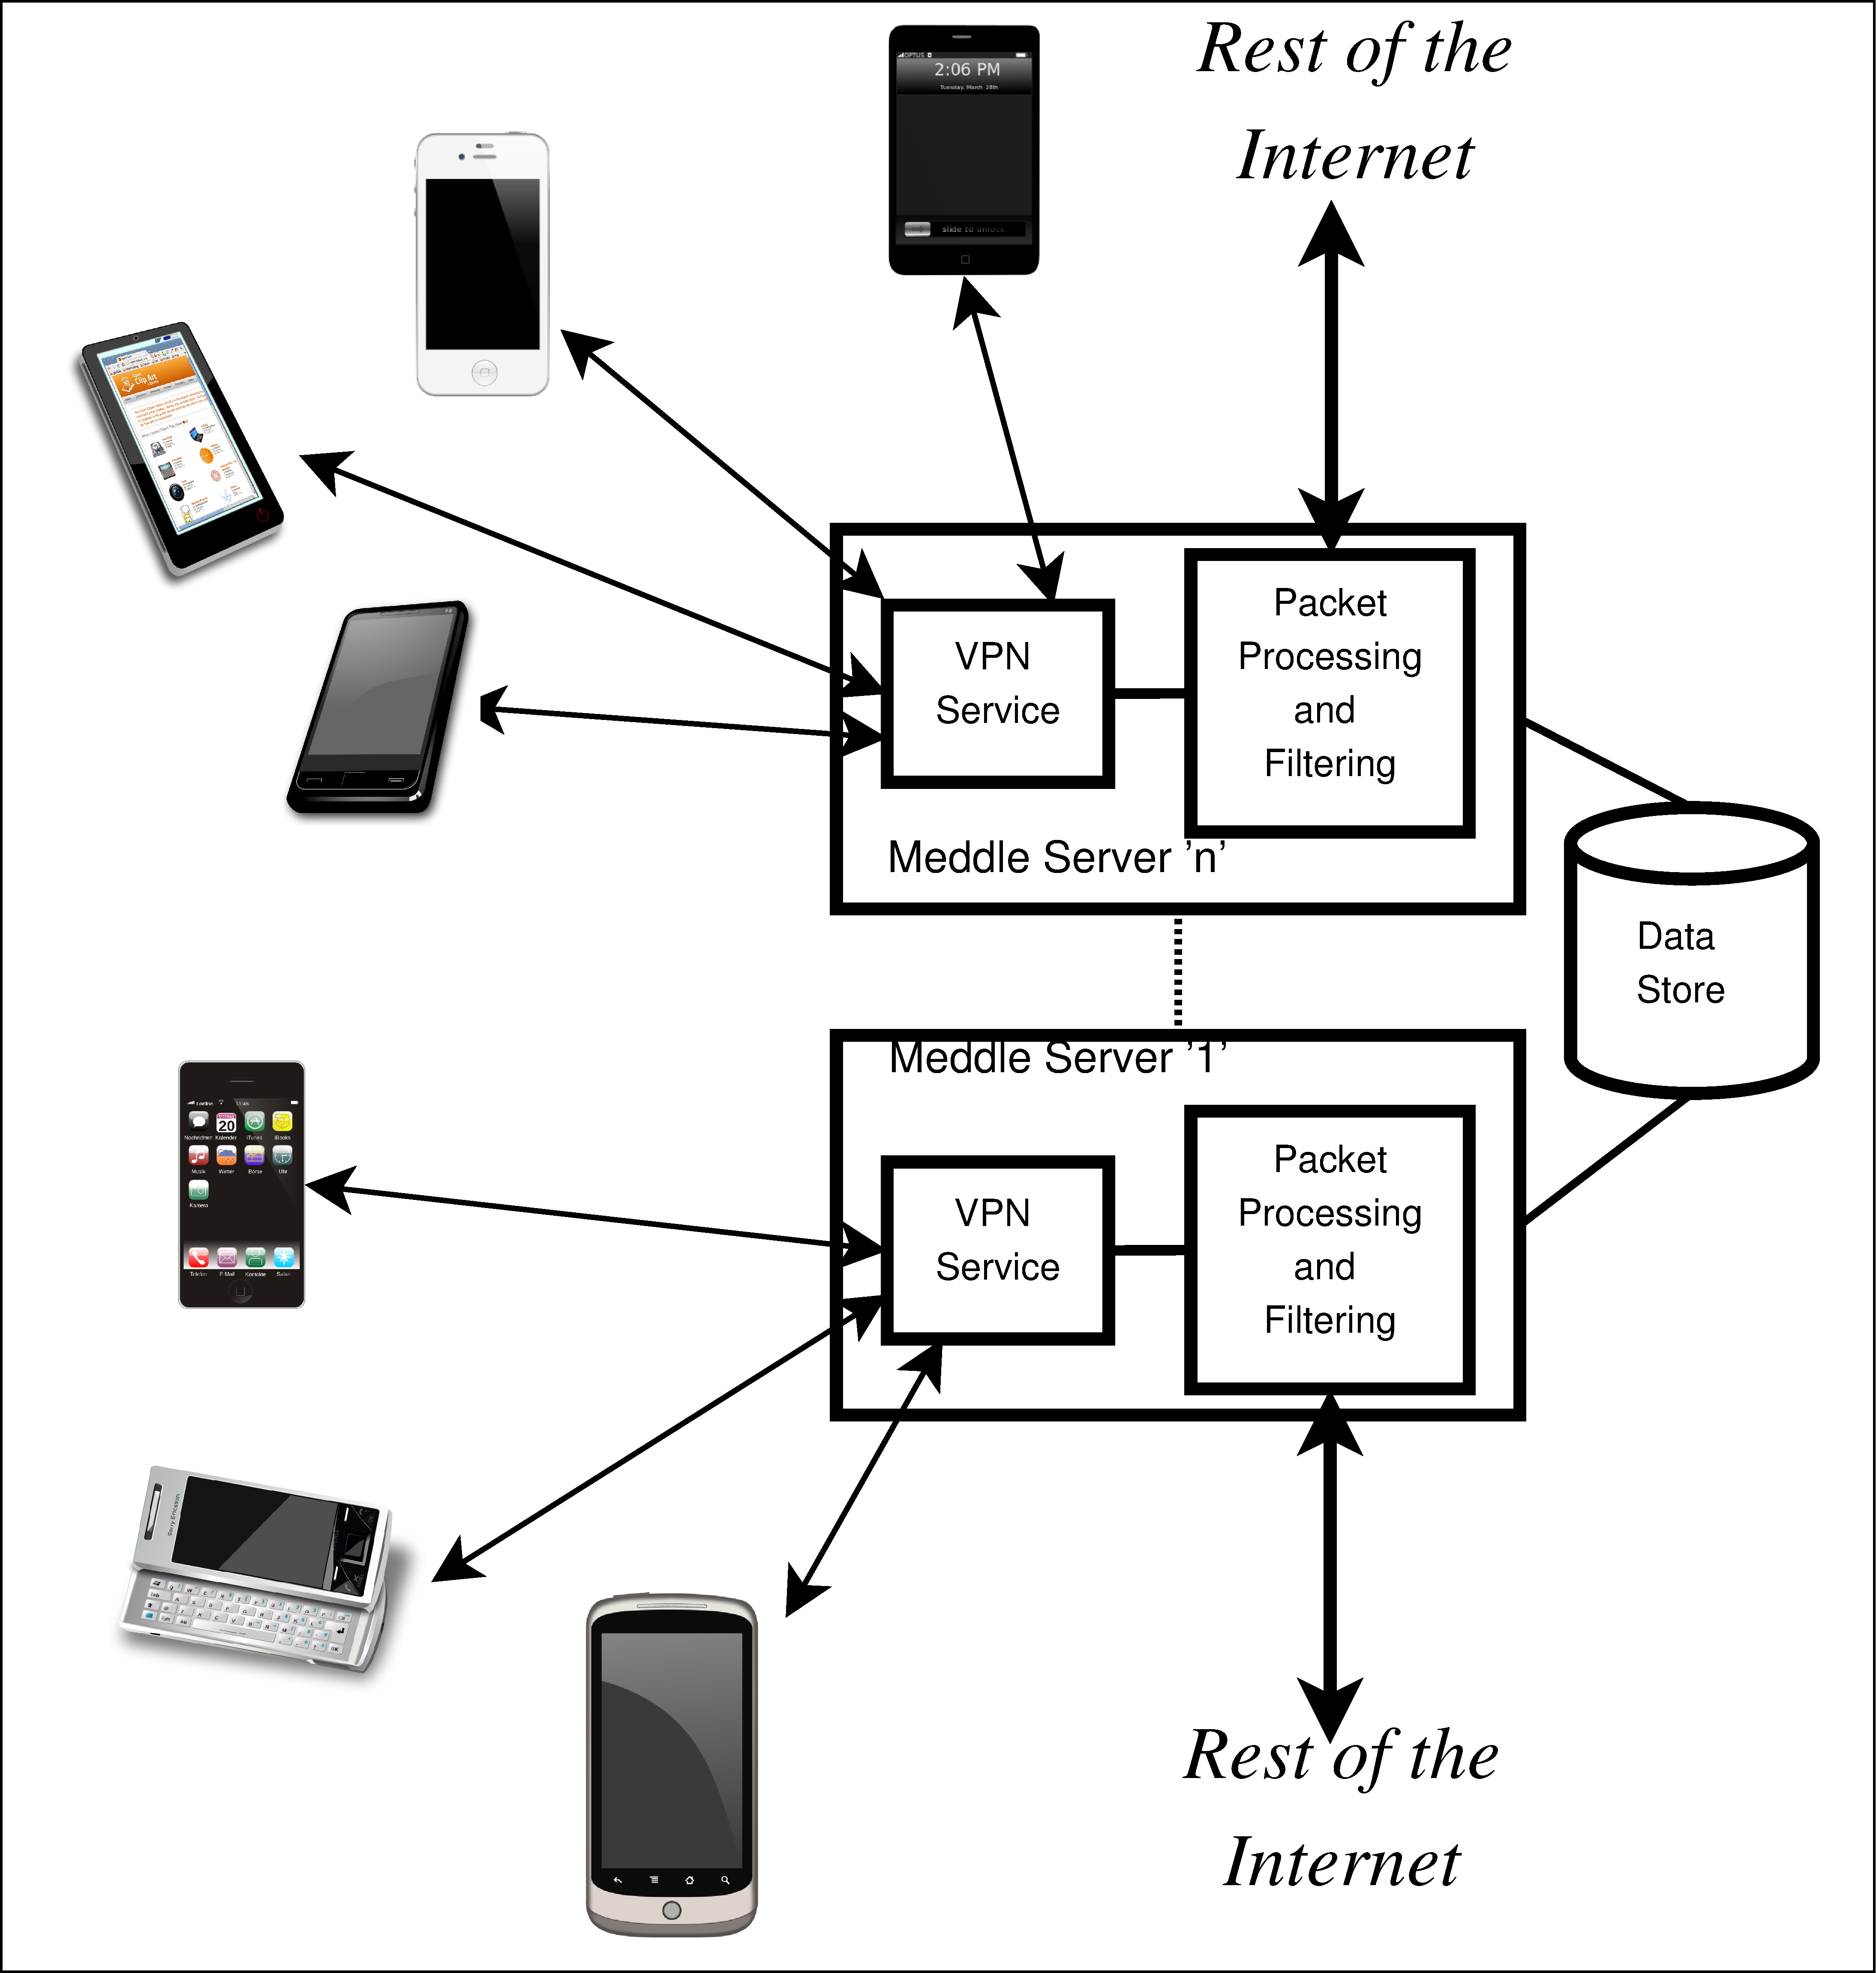
\includegraphics[width=0.8\linewidth]{figs/meddle-servers.pdf}
\vspace{\figcapspace}
  \caption{\meddle architecture. Devices use VPN connections to tunnel all 
  traffic to one of potentially many \meddle servers dynamically chosen to 
  optimize for performance. Each \meddle server uses a device- or user-specific 
  profile to determine the set of services that will operate on the tunnel's network traffic.}
  \label{fig:arch}
\vspace{\postfigspace}
\end{figure}

When a device attempts to connect to \meddle, we direct it to a nearby 
\meddle server in a similar way to how the Akamai CDN uses DNS to redirect 
Web clients to nearby content caches~\cite{akamai:cdn}. 
To optimize for performance, the service can send VPN clients to a 
server that is relatively near the location at which data exits
the mobile carrier's network to enter the Internet. This technique 
can also redirect clients based on server load, reachability and availability. 

To meet the goal of providing control over network traffic in the mobile 
environment, each \meddle
server uses software-middlebox techniques, or \emph{meddleboxes} to interpose on 
network traffic. These meddleboxes can (i) implement custom services for users such as packet
filtering, caching, and intrusion detection, (ii) monitor network
traffic characteristics, and (iii) allow us to experiment with alternative
algorithms and protocols for the mobile environment.
The system maintains a per-device and per-user profile 
to determine the set of services that will operate on the tunnel's 
network traffic. 

\tbd{Discuss the interior of a meddlebox.}

While the \meddle architecture is straightforward, there are a 
number of challenges we must address in building a viable deployment. 
In the next section, we describe how we achieve continuous monitoring 
of network traffic across platforms, demonstrate that the power, data-volume and latency 
overheads are reasonably small.







%DRC: These are the things I think we need to emphasize as key features
%
%Portable (Cross platform, access technology, provider w/o needing app or rooting)
%Continuous/Pervasive (always on)
%Passive (low cost, real traffic)
%Control


% - Increase transparency of the opaque mobile ecosystem
%   + Opaque because
%     - tied to OS, service provider
%     - limited knowledge of apps - measurement studies limited to small user set or data sets from cell providers
%     - no knowledge of what service providers are doing
%       - Trip wire 
%     - only way to address somes of these issues is to root the phone, but this cannot shed light on what carriers are doing
%   + Allow users to ensure they are getting what they pay for
%   + Prevent and/or monitor carrier interference
%   + Understand network footprint of apps and devices over time
% - Expose control knobs to enable users to tune the traffic 
%   + Control knobs exists on home gateways and people use it (DRC: Not sure we can prove anything about this)
%      - Firewalls on home gateways but none for mobile - direct exposure to internet 
%	DRC: This isn't true. Mobile networks are in a sense a giant firewall.
%      - Control knobs to filtering traffic given by iOS but details not publicly available (DRC: Mainly, these knobs are coarse-grained and insufficiently expressive to meet the intended goals of parental controls.)
% - Have a low barrier to entry
%   + Users do not want to violate terms of service (DRC: They want to, but are afraid to :-)
%   + Rooting/Jailbreaking issues - not easy, ROMs may not be available for device, opens device to huge security risks
% - VPN based middleboxes to achieve each of these goals
%** System Descripton
% - VPN based middlebox
%    - Why VPNs and advantages of VPNs 
%      + comprehensive view -- cross access technology, service provider, device
%      + native IPsec support on smartphones and tablets
%      + low barrier to entry -- no need to jailbreak phone or install custom OS
%    - - Summary
%    - We need strong statements here to indicate this is indeed feasible
%    - We can cancel the affects of these overheads by the value added services that we provide


\section{Implementation}
\label{sec:deploy}
In this section, we describe our current deployment, we discuss how we addressed several 
challenges toward achieving the goals listed in the previous section and 
we present empirical results demonstrating the feasibility of our approach 
in terms of reasonably low overhead. 

\subsection{Meddle Details}
The design of \meddle facilitates widespread adoption because it is supported out-of-the-box by the vast majority of smart mobile devices (smartphones and tablets) and is easy to deploy on servers. Manually configuring a VPN generally requires filling out five fields on an Android phone, and the VPN configuration can be distributed using a single file on iOS. These configurations are primarily required to drive the key exchange algorithms required to establish the VPN tunnels. The two most popular key exchange algorithms are IKEv1~\cite{rfc4109} and IKEv2~\cite{rfc5996}. Android devices support IKEv2 while iOS devices currently support only IKEv1 for tunnel establishment. The advantage of IKEv2 is that the VPN tunnel is generally established using 4 packets compared to 15 packets exchanged to establish the tunnel using IKEv1.

\noindent\textbf{iPhone support.} We support \meddle on iOS using the ``VPN On-Demand'' feature, 
introduced in version 3.0 of iOS. This was originally intended to allow enterprises to 
ensure their employees' devices always establish a VPN connection before contacting 
a specified set of domains. Using trial-and-error, we discovered that VPN On-Demand uses 
suffix matching to determine which domains require a VPN connection. 

We use each alphanumeric character as the set of domains that require a VPN 
connection. This ensures that a connection is established before \emph{any} network 
activity.

\noindent\textbf{Android support.} As of Android 4.2, Android supports 
``always on'' VPN connections that ensure all traffic is always tunneled. 
At the time of writing, this has been released only for one week and only 
for a subset of Android devices so we have not extensively tested the 
effectiveness of the solution. 

Instead, we rely on a feature that allows apps to manage VPN connections, 
introduced in Android 4.0. We modified the StrongSwan implementation of 
a VPN client~\cite{strongswanclient} to ensure that the VPN reconnects each time the preferred 
network changes (\eg, when a device switches from cellular to \wifi). 

\noindent\textbf{Server-side implementation.} In our current implementation, \meddle 
uses native IPsec, implemented via StrongSwan~\cite{strongswan}, to establish VPN tunnels 
and custom packet filters plus Vyatta middlebox software~\cite{vyatta} to shape
traffic. Both of these software artifacts are supported on vanilla
Linux operating systems, which in turn run on nearly all servers. 
   
\subsection{Feasibility}
\label{subsec:cost}
Because our approach in part depends on users installing a VPN configuration and tunneling all traffic through \meddle, we evaluate whether the cost to the user in terms of performance, power and data quota is sufficiently low.
  
\noindent\textbf{Data consumption.} IIPsec encapsulation slightly inflates packet sizes, in addition to 
preventing carrier middleboxes from applying their own compression. We measured the overhead 
of the tunnel in terms of data overhead from IPsec headers and keep-alive messages, finding that it 
ranges from 8--12.6\%. 

For our measurements, we capture the encrypted packets exchanged by 
our \meddle servers and the clients that use \meddle. We performed the packet capture for 14 days 
during which 20 devices tunneled their traffic via our \meddle servers. During this time interval we 
also capture the packets that were encapsulated in the IPsec packets. We use these samples to 
compute the increase in the amount of bytes transferred due to encapsulation and the keep-alive 
messages. During the 14 day period we observe that the median of the increase to be 8.23\%, 
with a maximum increase of 12.6\%.

\noindent\textbf{Performance.} By forcing user traffic to an
intermediate server and interposing on flows, we may add latency both
due to additional hops and due to processing time at the \meddle
server. We envision a DONAR-style deployment where users are
dynamically redirected to different \meddle servers based on network
conditions and server load~\cite{wendell:donar}. Given this model, we
evaluate whether we can locate servers near mobile-network egress
points using a deployment such as PlanetLab, and found that this is
generally the case.

For this experiment, 
we used data from approximately 10 mobile phones located throughout
the US and issued traceroutes from the devices to targets in Google
and Facebook's networks. We then used the first non-private IP address seen 
from the mobile device on the path to a server. We assume that this corresponds 
to the first router adjacent to the mobile carrier's public Internet egress point. Note that we could not simply ping the device IPs because mobile carriers filter inbound ping requests. Using this set of egress adjacencies, we determined the round-trip time from each PlanetLab site, then took the average of the nearest five sites to represent the case where a host at the nearest site is unavailable due to load or other issues. The average latency to each router was between 3\,ms and 13\,ms, with a median of 5\,ms. Thus, when compared to RTTs of 10s or 100s of milliseconds that exist in mobile networks, the additional latencies from traversing \meddle servers is expected to be relatively small or even negligible.

\tbd{What is the cost in terms of end-to-end performance?}

\tbd{Are there cases where we actually improve performance due to
detouring? (I've decided not to mention this because it's not a sure thing.)}
\tbd{In case the carrier is performing traffic differentiation to
  penalize some bandwidth consuming traffic, using a VPN might
  significantly improve performance. I don't know whether traffic
  differentiation is something common on mobile networks. (that was an
  answer to Dave question. If he discards it, also drop my comment.) }


\noindent\textbf{Power consumption.} Tunneling traffic to a \meddle
server requires that all traffic be encrypted by the mobile
device. While this is already commonly performed for SSL connections,
\meddle requires an \emph{additional} layer of encryption. We observed
a 10\% increase in power consumption when streaming an HD video to
Android and iPhone devices using our IPsec tunnel. We believe that this 
overhead is reasonably low, and we note that this cost for encryption comes with the added benefit of increased 
privacy from third parties. To put the overhead in context, the iPhone 5 advertises 
8 hours of LTE browsing per charge; with the VPN enabled this would reduce to 
7 hours and 12 minutes.

An interesting research question is whether it is possible to \emph{reduce} power consumption using \meddle. For example, Qian et al~\cite{qian:rrc,qian:aro,qian:periodic} found that traffic shaping (a service that \meddle provides) can significantly reduce the power consumed by devices when periodic application traffic and radio resource timers are out of sync.

\noindent\textbf{Scalability.} If wildly successful, we would like to
ensure that \meddle scales gracefully and that there are sufficient
resources to support large numbers of concurrent users
worldwide. Based on our initial analysis using StrongSwan on commodity
hardware, we found that each connection consumed on average less than
1\% of CPU time. Thus, we expect to be able to support up to hundreds or
small number of thousands of users per server, which is in line with
low-end VPN appliances sold by Cisco and Vyatta. A recent
study~\cite{pcworld-speedtests} showed that current rates for 3G
networks in the US were between 0.59 and 3.84 Mbps; assuming devices
are uniformly distributed across carriers, we expect to be able to
support 250 simultaneous users (saturating their download capacity)
for every 1 Gbps of bandwidth at the server.

\subsection{Current Deployment}
\label{subsec:currdeploy}
The analysis in the following sections relies on data gathered from 
our current prototype deployment. This consists of \meddle servers at the University of Washington, 
UC Berkeley and Inria, along with 20 devices from 14 users participating 
in an IRB-approved study. 

\noindent\textbf{Summary statistics.} \meddle has been running 
since September 2012. The deployment includes 8 Android devices 
and 12 iOS devices (4 iPads, 7 iPhones and 1 iPod Touch). These 
devices connect to \meddle via 15 different service providers, 
four of which are cellular providers. Together, our users have 
generated 30.2\,GB of traffic since November 1, 2012. 

\noindent\textbf{Data collected.}
We collect full packet traces from these users 
(with informed written consent) and we code the data using random identifiers 
to protect identities. We do not attempt to decrypt any SSL traffic, 
and all packet traces are encrypted using a public key before being 
stored on disk. The private decryption key is stored on a separate server. 
Users may opt out and choose to delete their data at any time. 



   

 
 
%  IPsec support on mobile devices 
%       + IKEv1 with Certificates for iOS and Android
%       + On demand on iOS fully supported
%       + Android 4.2 has always on but not on demand 
%           - short comings on IP and not host names
%           - no IKEv2 support - faster and less connection 
%       + Strongswan APP 
%           - support ICS, and Jellybean  
%           - added functionality to have always ON
%       + Strongswan on the server 
%           - Native IPSec support, 
% - Servers in UW, berkeley, and Inria. 
% - Openvswitch based middleboxes ?? (Justines inputs needed here) 
%** System Feasibility
% - VPNs by Smartphones
%   - IKEv1 and IKEv2 
%   - Short VPN Primer comes here 
% - Network overheads (data and latency)
%   - Signalling overheads - from Strongswan   
%   - Headers in each packet - from IPsec standards 
%   - Other overheads
%   - (Ideas for VPN issues and improvements of VPN for Mobile networks)
% - Power overheads (Inputs from Aruna on the time required to perform these tests)
%   - Cannot do this for iOS but we can do a test with power up and down
%   - Power meter setup
%      - Devices used in the test            
%   - Test case description ( Do we have time for this??)
%         - factory reset the device (stop all apps that have been installed by the user)
%         - Perform the test with and without VPN
%              - browse the web with and without VPN - Select websites domain from alexa top sites
%              - Install 5 most popular games from the store for atleast 15 minutes
%              - Listen to Music, Pandora, TuneIn radio (1 hour per app -- about 10 songs to include ads)
%              - See 5 videos from YouTube                  
%   - Test results
% - User Concerns and Security Risks (do we need it here??)
%   - Privacy implications - IRB to ensure user privacy is not violated
%   - Server failures - VPN tunnel shall not be established but  
%   - EULA that allows us to block malicious user activity


%\section{Measurements}
%\label{sec:measurements}

\eat{All the subsections are now sections. We can merge them later}

\section{Network Characteristics of Notification Services}
\label{sec:characterize-os}

Mobile operating systems provide OS level notification services to optimize network usage.
The Apple Push Notification service (APNs) and Google Cloud Messaging (GCM)~\cite{gcm} are used by iOS and Android applications respectively to receive notifications from the Internet.
In this section we show how \platname was used to compare the notification services of iOS and Android, and detailing it behavior in the wild. 

\begin{figure}
\centering
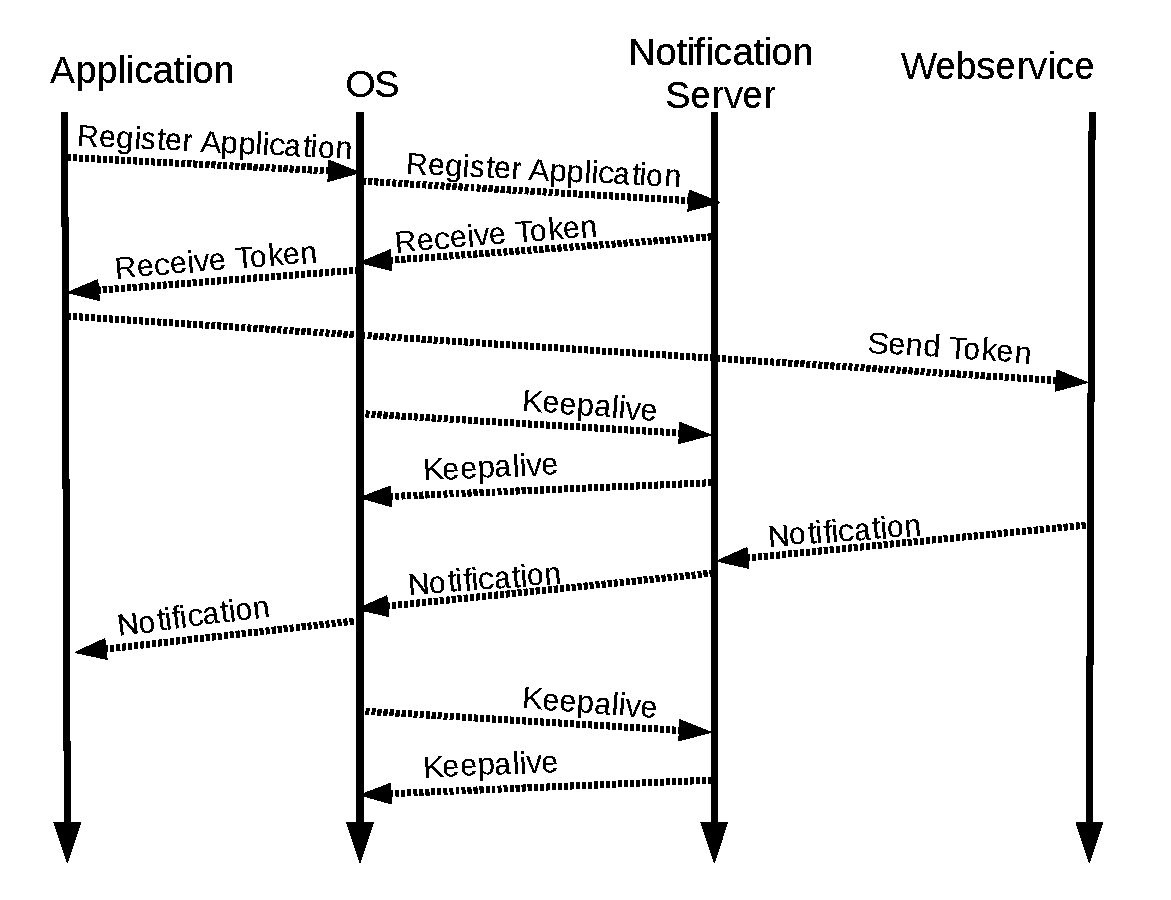
\includegraphics[width=\columnwidth]{figures/Notification.pdf}
\caption{Notifications on mobile OSes. \emph{Because notification messages are sent over TCP, keepalive messages are periodically exchanged to ensure TCP connections do not timeout.}}
\label{fig:push-expt-interarrival}
\end{figure}



\subsection{Controlled Experiment on Factory Reset Devices}

We first detail the detail the behavior of notification services by performing a controlled experiment on \emph{factory-reset} devices. 
The objective of this experiment was to analyze notification services for devices that are used \emph{out of the box}, and detail the impact of device manufacturer, and pre-installed applications. 

For our experiment, we performed a \emph{factory reset} on an iPod Touch, an iPad, an iPhone, a Samsung Galaxy SIII, and a Google Nexus S Phone; the reset was performed after their batteries were fully charged. 
We then perform the initialization step and assigned a dummy email account as the primary account to each of these devices.
We then allowed these devices to connect to the Internet over \wifi through \platname and monitored the Internet traffic from these devices.
We then studied the impact of access technology by letting the iPhone and Samsung Galaxy SIII tunnel traffic through \platname using cellular networks. 

We observed that the traffic volume during the 24 hour periods varied from 19~KB to 97~KB depending on the devices. 
We classify APNS and GCM messages using the TCP port numbers mentioned in their specifications~\cite{gcm, apns}.
Because we did not run any applications in the foreground, notification messages were responsible for largest fraction of the traffic volume; the share was 35\% for Nexus S, 88\% for the Samsung SIII and around 50\% for each of the iOS devices. 
The share of DNS traffic varied from 10\% to 40\% for each of the devices while the other services contributed to less than 10\% of the traffic volume.
The only exception was the Samsumg Galaxy SIII which used location services that contributed to 26\% of 47~KB traffic volume generated by the device.

\begin{figure}
\centering
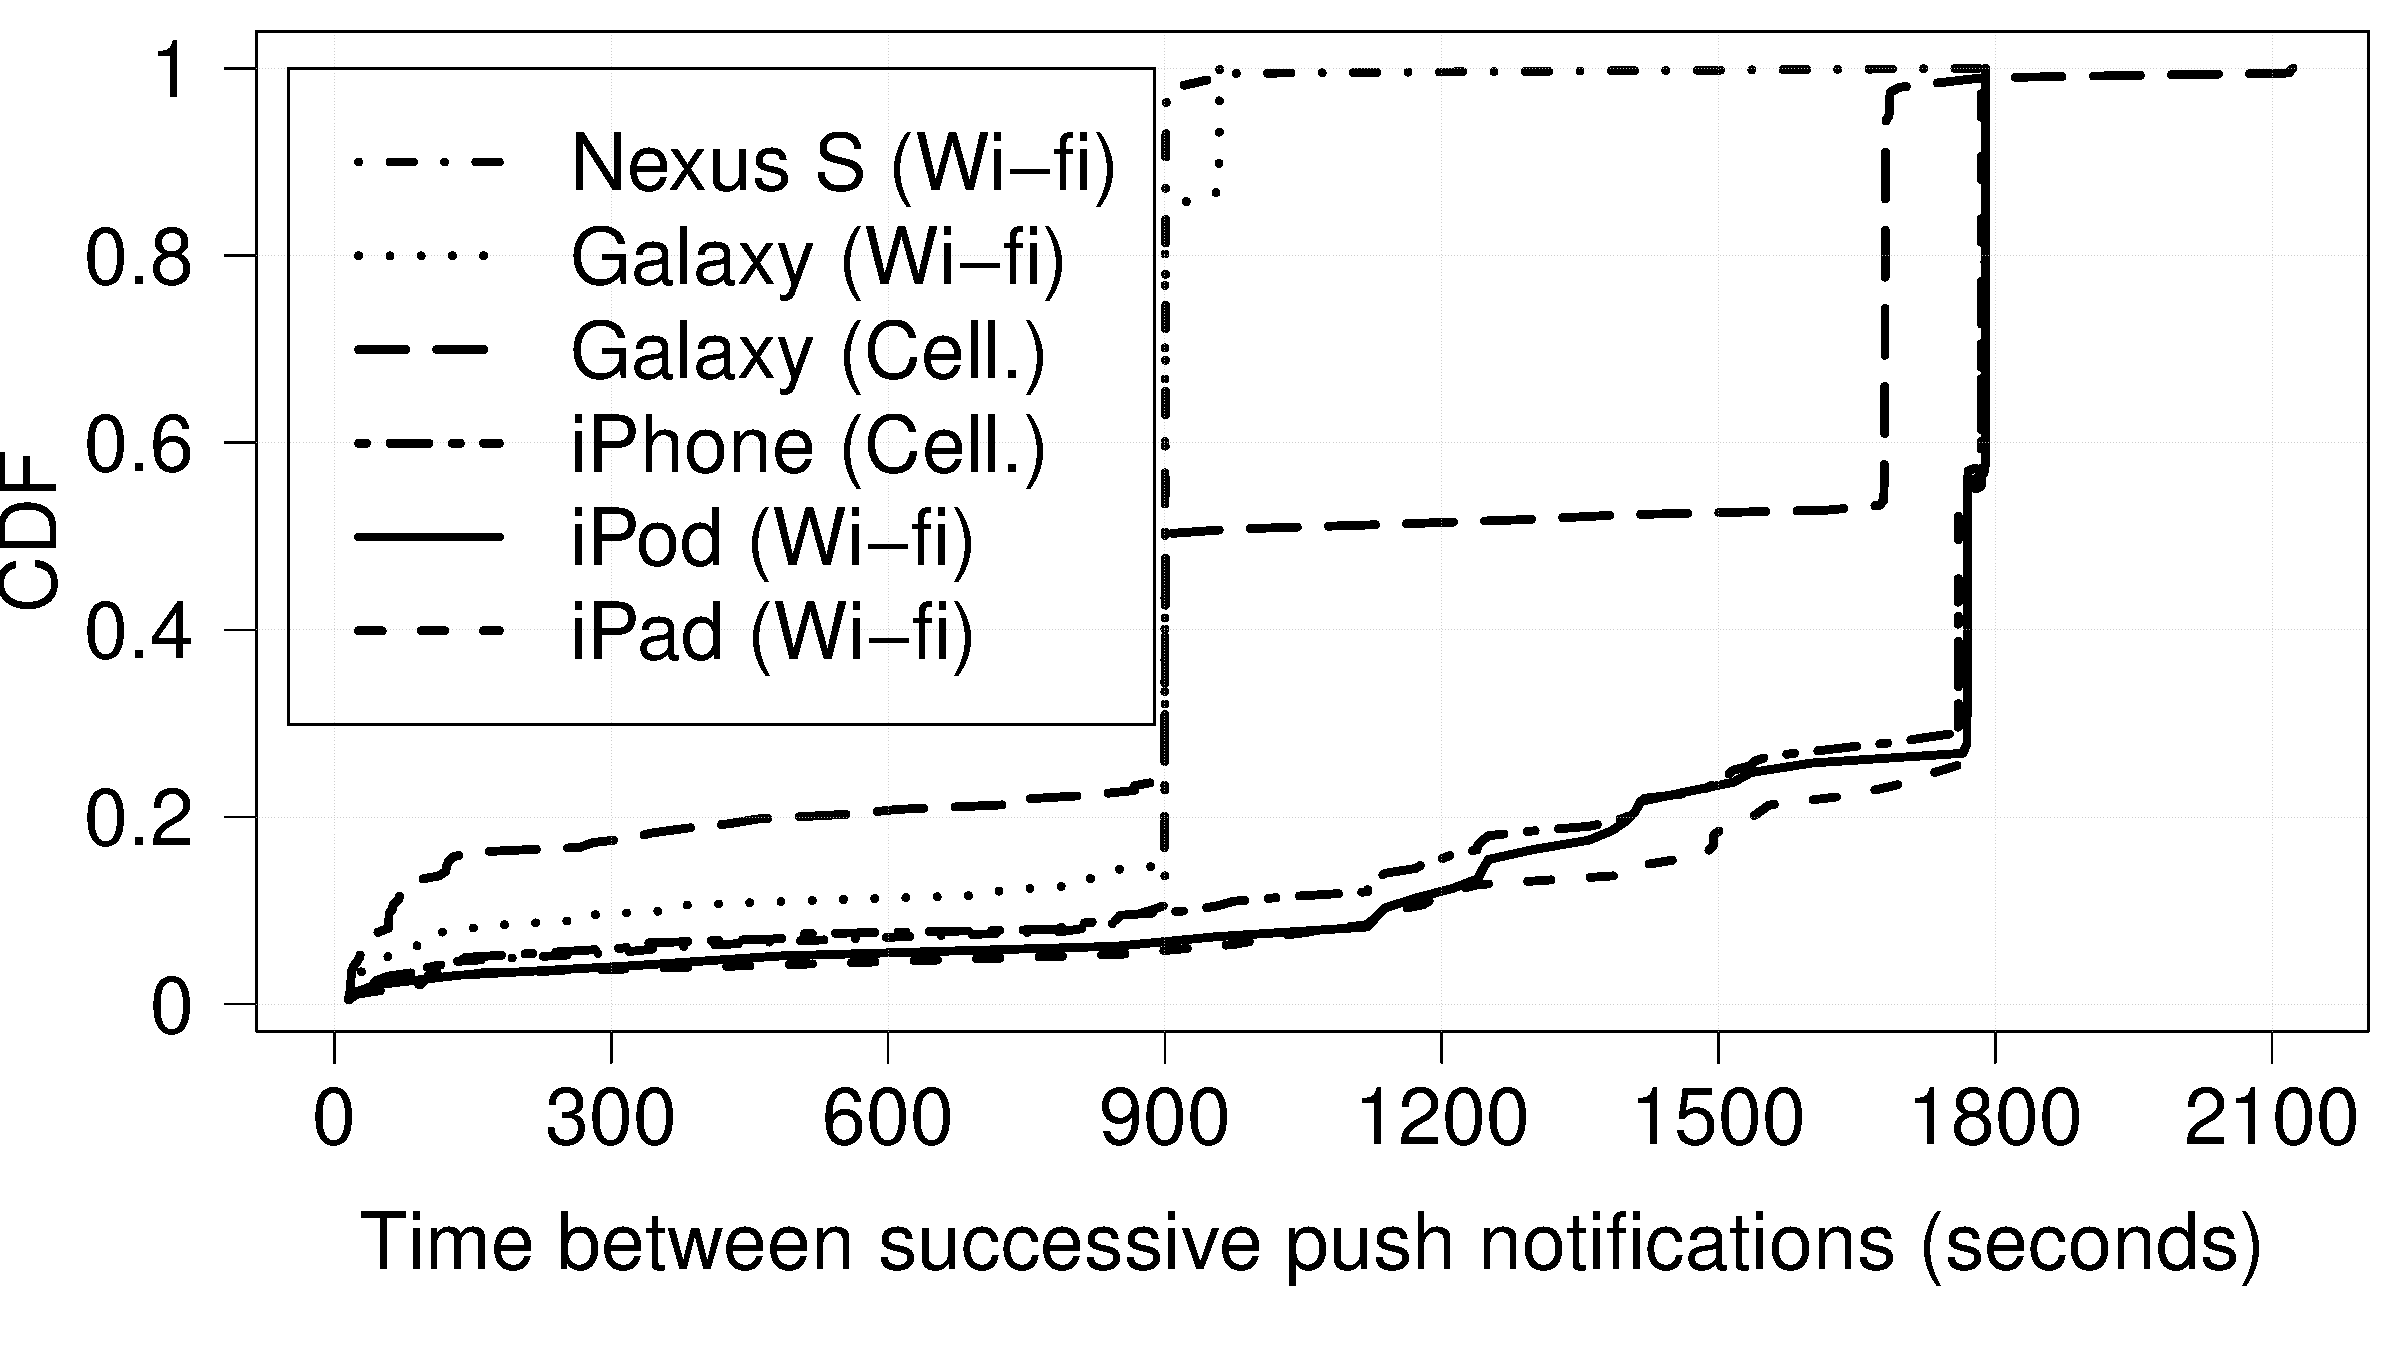
\includegraphics[width=\columnwidth]{plots/push_factoryreset_interarrival_distrib.pdf}
\caption{Inter-arrival time between notification messages after factory reset. \emph{The Android and iOS devices communicate with the notification server approximately once every 900~seconds and 1800 seconds respectively. The behavior of Android devices depends on the device, the pre-installed applications, and the access technology.}}
\label{fig:push-expt-interarrival}
\end{figure}

In \fref{fig:push-expt-interarrival} plot the time between successive messages sent by the notification servers on the ports assigned for notifications. 
We observe that the inter-arrival time between notifications for the Android devices is at least 900 seconds for more than 80\% of the notifications observed. 
The distribution of the inter-arrival time also depends on the access technology for the Samsung Galaxy SIII phone; we observe steps in the distribution for the SIII phone while we do not observe these steps when the same phone uses \wifi. 
We do not observe this difference when the Nexus S phone used the cellular data connection; we do not present the figure due to lack of space. 
\tbd{AR: Why these difference -- which applications stop coming up and so on}.
For the iOS devices, we observe an inter-arrival time at least 1700~seconds for that more than 75\% of the notifications in \fref{fig:push-expt-interarrival}. 
We do not observe a significant difference between the inter-arrival times for the iPhone over cell and \wifi and we do not present these results due to lack of space. 

On analyzing the packets exchanged, we observe that  all Android flows with an inter-arrival time larger than 800 seconds consisted of an empty TCP packet sent by the device followed by a 25 byte payload sent by the server.
Similarly, all iOS flows with an inter-arrival time larger than 1500 seconds began with an TCP packet with a payload of 85 bytes sent by the device followed by the server responding with of a TCP packet of 37 byte payload.

In summary, we observe notifications consume very little data, less than 50~KB in 24 hours, on Android and iOS devices in their default state.
The large time between successive notifications and the small amount of data exchanged implies they consume very little power.
We also observe that iOS devices have a larger time between successive notifications compared to Android devices in the default state. 
Furthermore, the inter-arrival time between notifications for Android devices differs based on the device manufacturer and the access technology. 

\subsection{Notifications In The Wild} 

We now characterize our observations on the notifications we observed in the \mobWild dataset. 
The objective of this analysis was to detail the frequency, traffic volume, and source of the notification services. 

\begin{figure}
\centering
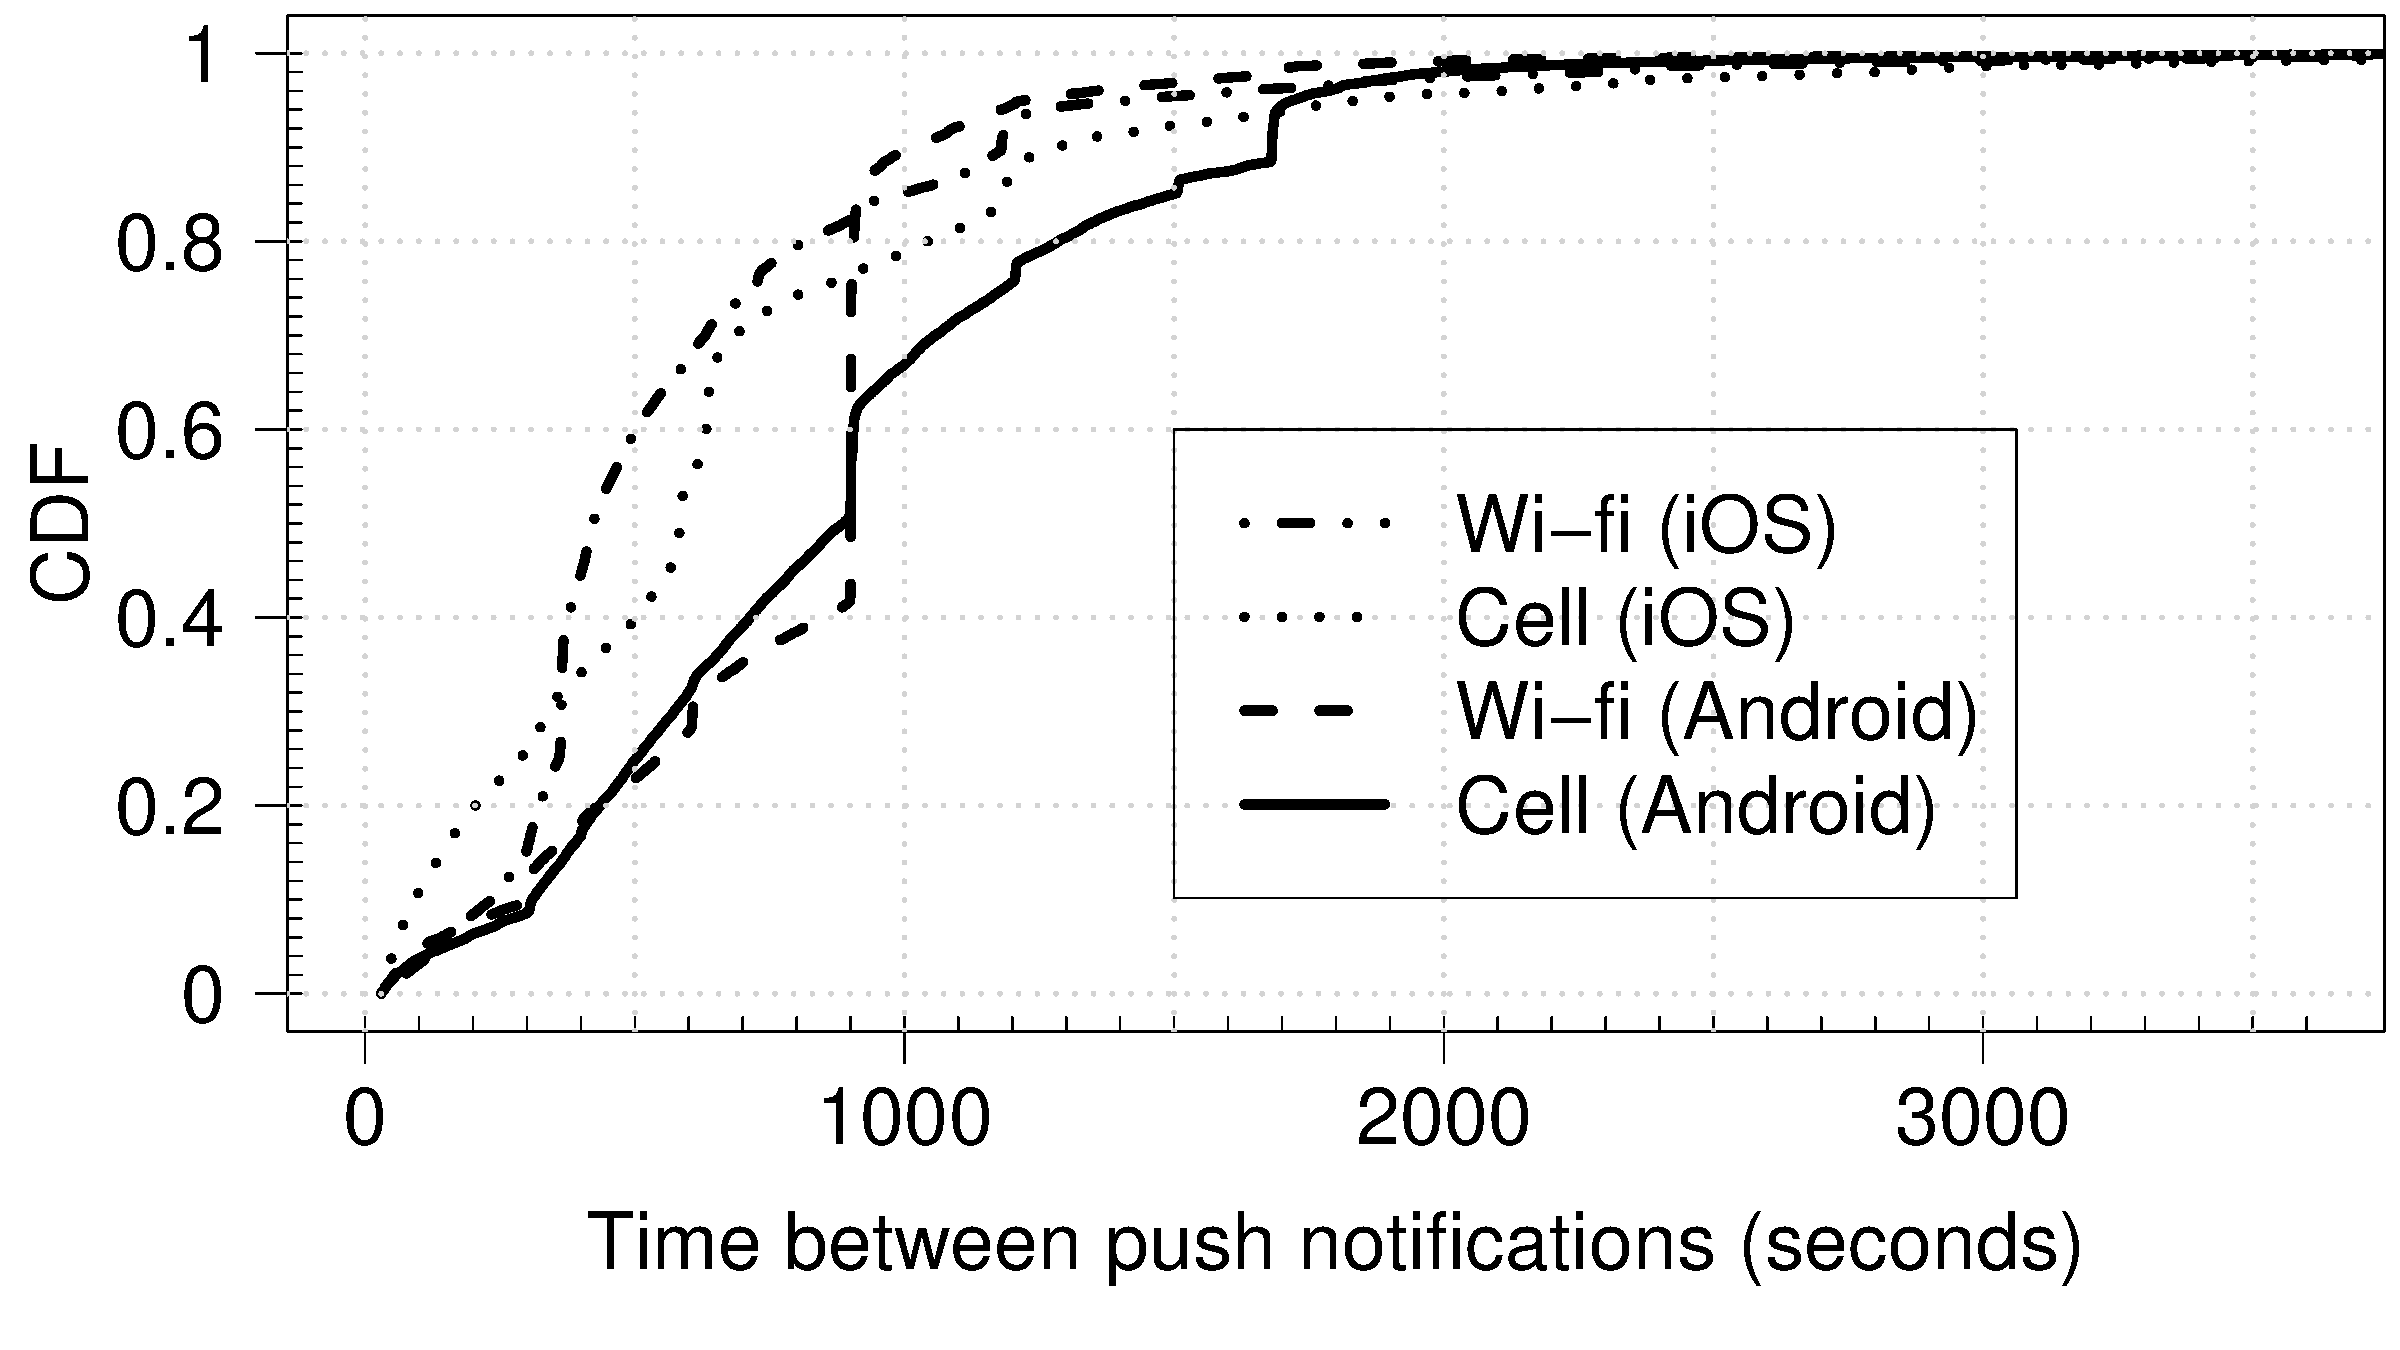
\includegraphics[width=\columnwidth]{plots/push_compare_os_tech_wild_distrib.pdf}
\caption{Distribution of the time between push notification messages in the wild. \emph{The frequency of push notification messages is higher for the iOS devices in our dataset compared to the Android devices. Notification messages are less frequent over cellular networks compared to Wi-Fi networks.}}
\label{fig:push-wild-compare-ostech}
\end{figure}

%The advantage of \platname is that it allows for direct comparison between devices across and their behavior across access technologies. 
To analyze the frequency of notification messages, we plot the distribution of the time between successive push notification messages for Android and iOS devices over cellular and \wifi networks in \fref{fig:push-wild-compare-ostech}.
In \fref{fig:push-wild-compare-ostech} we observe that a higher time between push notifications over cellular networks in comparison to \wifi networks for iOS and Android devices.  
We also observe the Android devices in our dataset receive notifications less frequently compared to the iOS devices in our dataset. 
We also observe a heavy tail for the time between notification messages which implies potentially long idle intervals.
\tbd{Correlation between time between notification messages and size of the next idle time observed?}


\begin{figure}
\centering
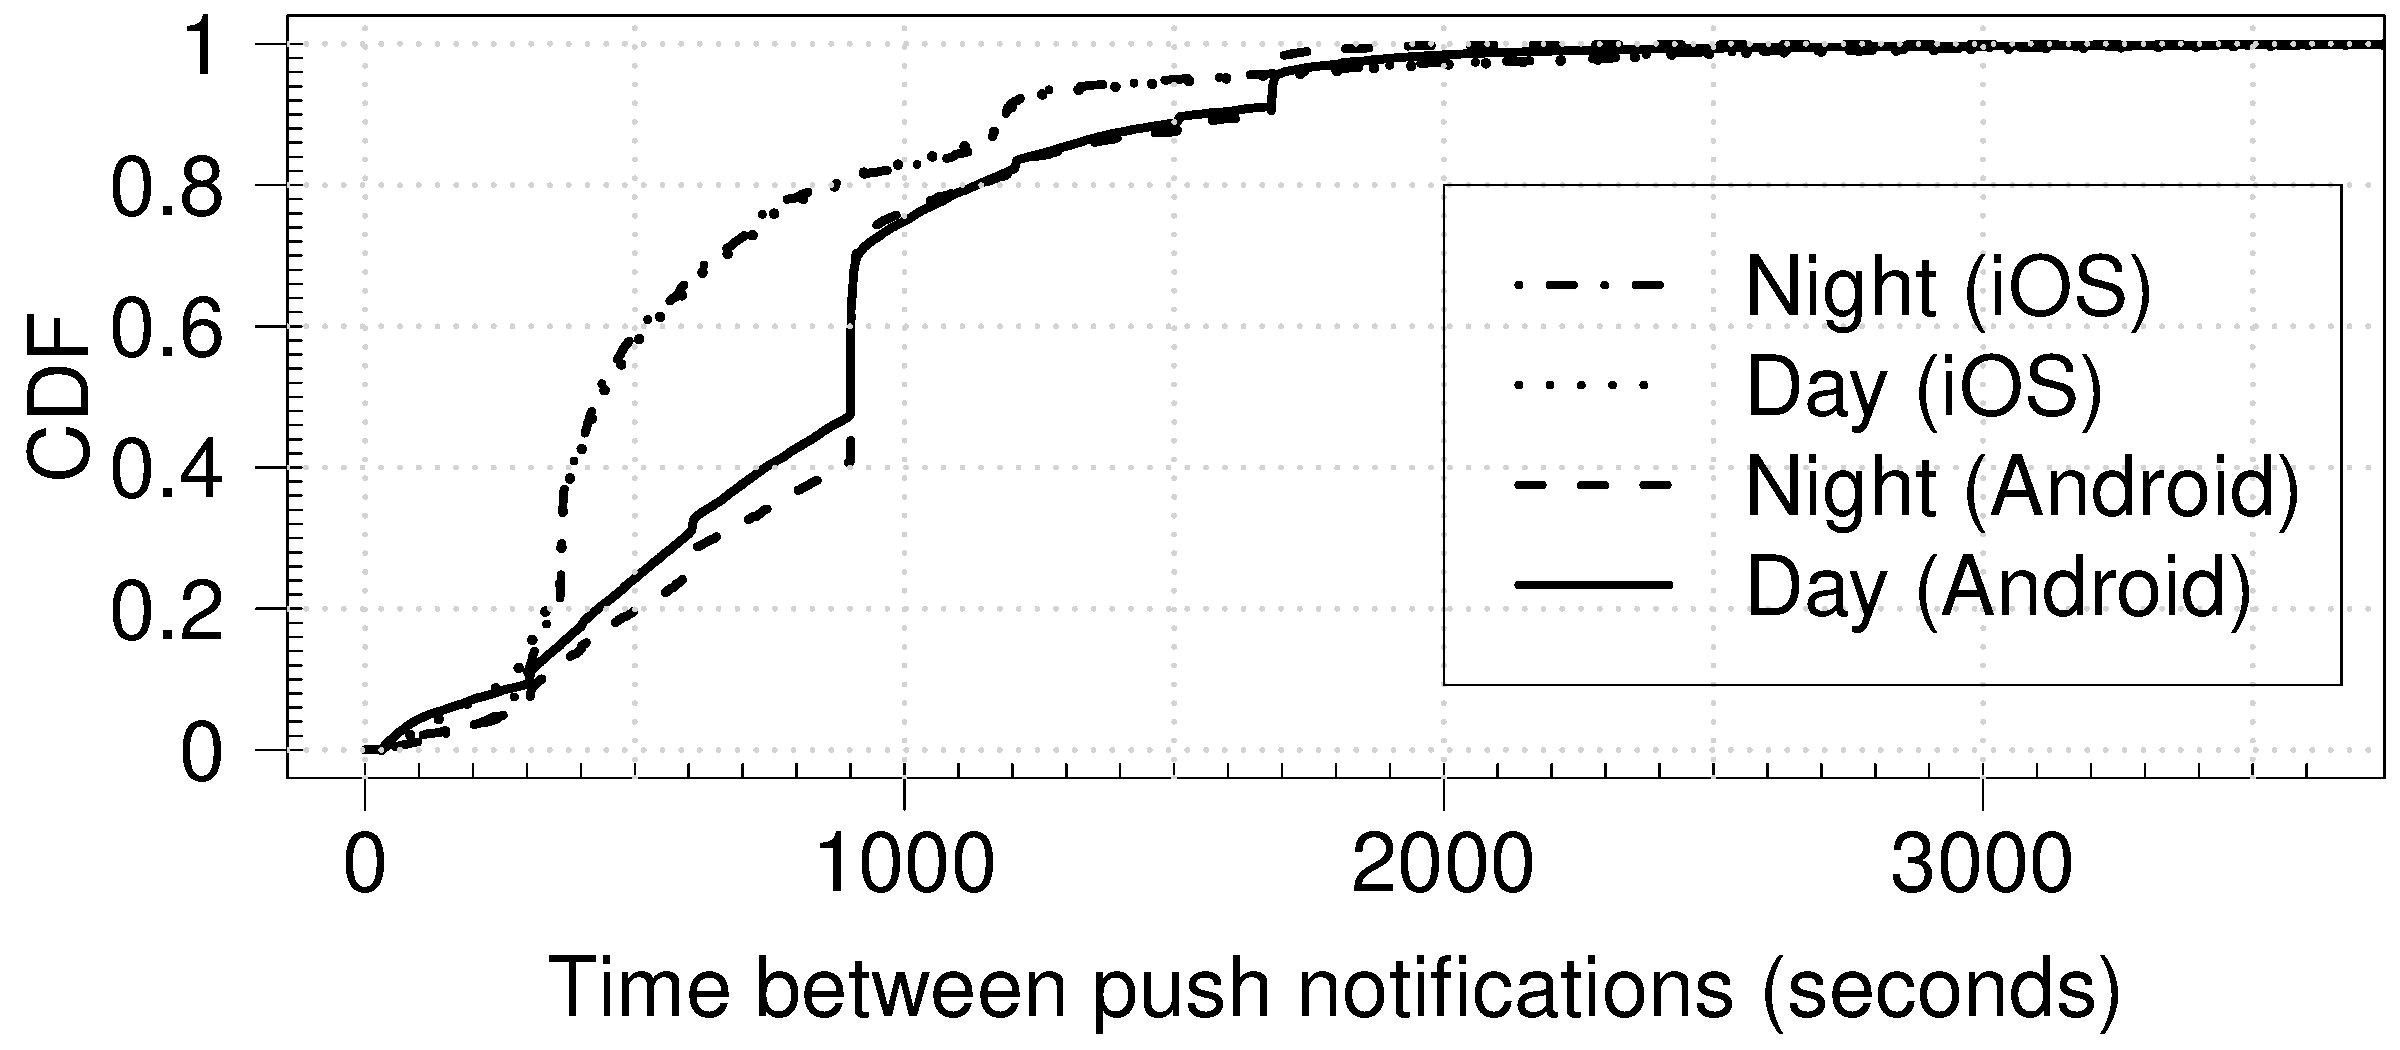
\includegraphics[width=\columnwidth]{plots/push_compare_diurnal_wild_distrib.pdf}
\caption{Impact of time-of-day on the push notifications. \emph{The rate of notifications is agnostic of the time of the day for iOS and Android devices.}}
\label{fig:push-wild-diurnal}
\end{figure}

The notification messages could be in response to user actions, for example, a mail server might receive a notification of a new message.
To analyze this impact, we notification messages received during two time intervals: from midnight to 6 am (night), and from 6 am to midnight (day). 
In \fref{fig:push-wild-diurnal}, we plot the distribution between successive notification messages for these two intervals. 
We observe that the Android and iOS devices appear to be agnostic of the time of the day. 
The iOS devices (from verion 6.0) come with a feature called \emph{Do Not Disturb (DND)} that does raise notification alarms on receiving notifications during specific time periods. 
We observe notification messages were received by the device that had enabled this feature during the intervals their users had configured as \emph{Do Not Disturb}.

\begin{figure}
\centering
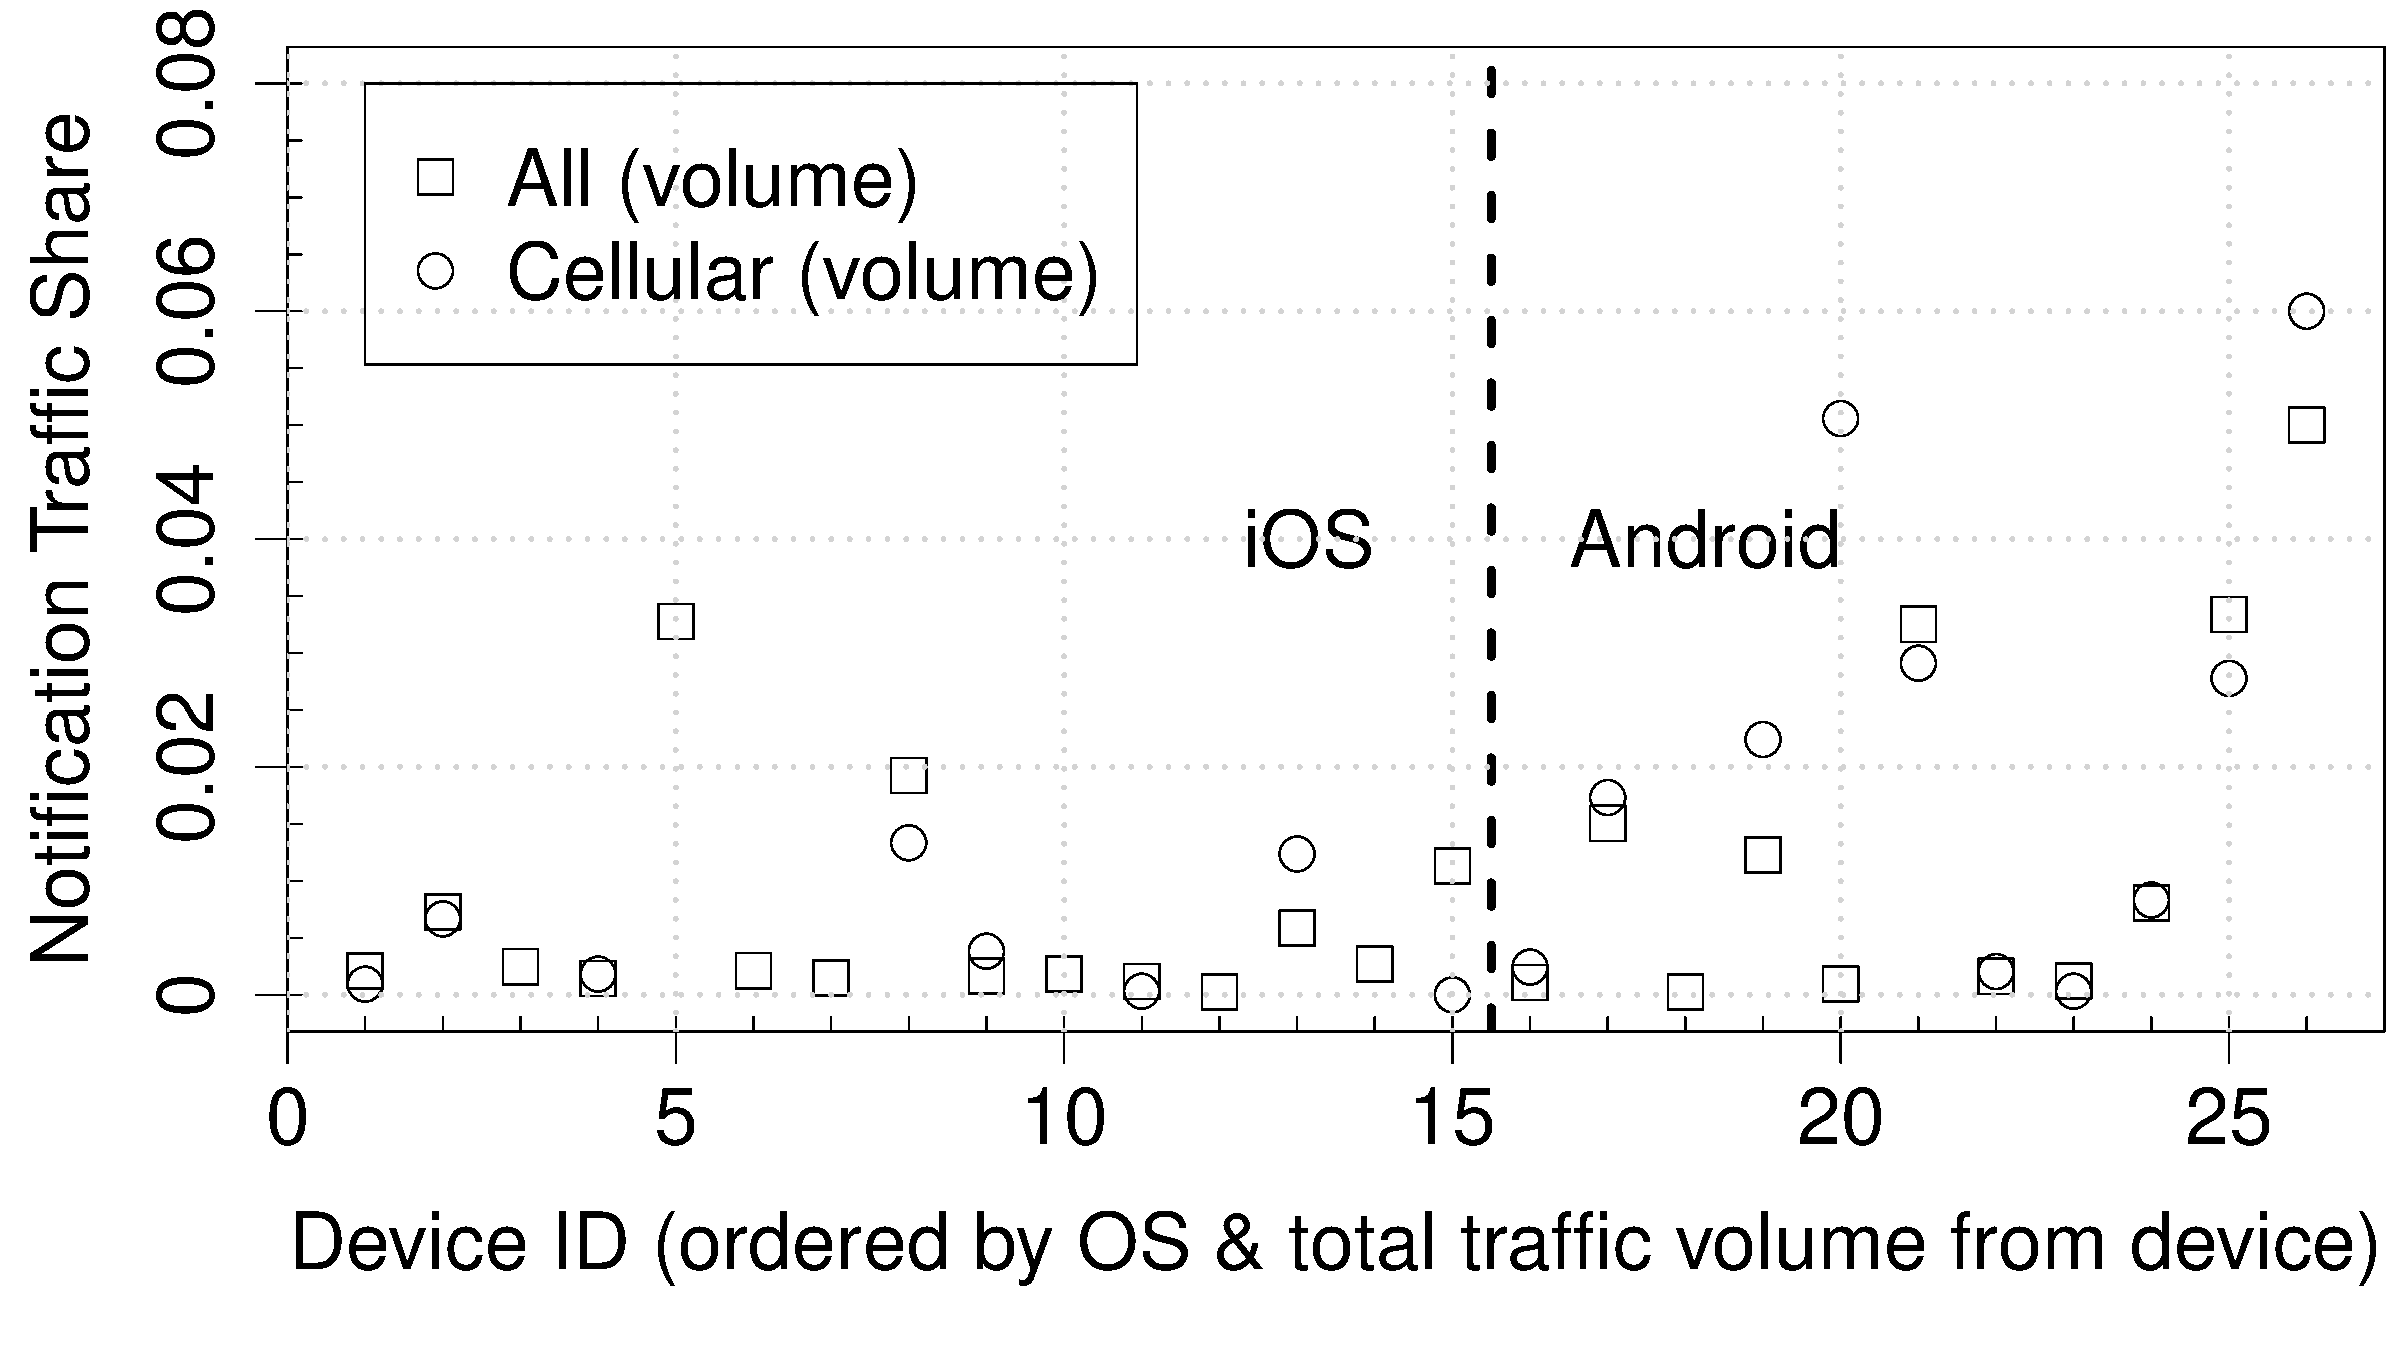
\includegraphics[width=\columnwidth]{plots/push_compare_trafficshare.pdf}
\caption{Traffic share of push notifications. \emph{Push notifications are responsible for less than 5\% of the traffic volume on most devices.}}
\label{fig:push-traffic-share}
\end{figure}

To analyze the volume of notification messages, we plot the share of notification messages as a fraction of total traffic from the device in \fref{fig:push-traffic-share}.
We observe that the notification messages are responsible for less than 4\% of the traffic volume on most Android and iOS devices. 
In \fref{fig:push-traffic-share}, we also plot the share of notification messages when the device exchanged data over cellular networks. 
We observe that there is no significant difference in the traffic share of notification messages when the device used cellular traffic. 
\tbd{Why do we care?}

To further analyze the source of the notification messages we analyzed the DNS lookups that were performed before the connections for receiving notification messages was established. 
We observed that the servers that pushed content to iOS devices correspond to the DNS requests that match the pattern \emph{*courier.push.apple.com} and \\ \emph{*courier-push-apple.com.akadns.net}.
For the android devices we observe that the DNS requests match the pattern\\ \emph{*talk.google.com}. 

In summary, we detail the behavior of the notification services using controlled experiments and the \mobWild dataset.  
We observe that push notifications consume a small fraction of the data and exhibit a heavy tail for the time between successive messages. 
We also observe that the frequency of notification messages was agnostic of the time of the day. 
Furthermore, notification messages were received by iOS devices even during the time interval the users had configured \emph{Do Not Disturb.}


% \begin{packedenumerate}
% \item How frequently do Push notifications take place in the wild?
% \item What is the impact of access technology on push notifications?
% \item What is the impact of the time of the day?
% \item What is the volume of push notification traffic?
% \item From which hosts are these notifications received?
% \end{packedenumerate}

%\subsection{Discussion}




% OLD TABLE WITHOUT IPHONE
% \begin{table}
% \begin{small}
% \begin{tabular}{|c|c|c|c|c|}
% \hline
% \multirow{2}{*}{\bf Application} & \multicolumn{4}{c|}{\bf Traffic Share in the first 24 hours}\tabularnewline
% \cline{2-5}
%      & iPad & iPod & Galaxy SIII & Nexus \tabularnewline
%      & (19 KB) & (21 KB) & (47 KB)& (97 KB)  \tabularnewline
% \hline
% Notifications & 0.54 & 0.53 & 0.35 & 0.88 \tabularnewline
% \hline
% Location & 0 & 0 & 0.26 & 0 \tabularnewline
% \hline
% SSL & 0 & 0 & 0.30 & 0.11 \tabularnewline
% \hline
% Mail & 0.05 & 0.07 & 0 & 0 \tabularnewline
% \hline
% HTTP & 0.13 & 0 & 0.09  & 0 \tabularnewline
% \hline
% UDP & 0.28 & 0.40 & 0.01 & 0.01 \tabularnewline
% \hline
% {\em total}& {\em 1.0} & {\em 1.0} & {\em 1.0} & {\em 1.0}\tabularnewline
% \hline
% \end{tabular}
% \end{small}
% \caption{Network usage in the first 24 hours after factory reset. \emph{Notifications contribute to the largest fraction of traffic volume across all devices.}}
% \label{tab:traffic-share-factory-reset}
% \end{table}

%While computing this distribution, we account the diversity in device usage in the following manner.
%For each device and each access technology we compute the 100 quantiles from 0.01 to 1.0 in steps of 0.01 of the time between successive push notifications. 
%We then use the median value of each quantile (from 0.01 to 1.0 in steps of 0.01) for a given access technology and operating system of the device.

% In \fref{fig:wild-inter-arrival-push} we present the time between successive push notifications for the 25 devices in our dataset. 
% As observed in \fref{fig:wild-cdf-push} we observe that the iOS devices receive push messages more frequently that the Android devices. 
% We also observe that the time between push notifications is higher for Android devices.
% The iOS devices prefer a cellular data connection for Push notification over \wifi \tbd{http://support.apple.com/kb/TS4264}. 
% However, in \fref{fig:wild-cdf-push} and \fref{fig:wild-cdf-push} despite this preference, we observe that the time between successive push notifications for iOS devices is higher over cellular networks in comparison to \wifi networks.  
% We observe that \tbd{SSL traffic} to mail servers was followed \tbd{x\%} after push notifications.
% This implies that higher usage of the device over \wifi may result in a higher number of notificatons received. 
% In \fref{fig:wild-inter-arrival-push}, device ID 
%Only if the cellular connection is not available or viable will the device switch to Wi-Fi for APNs connections.


\section{Application Characterization}
\label{sec:characterize-app}

  We now turn to measurements of specific popular iOS and Android applications. 
  When users install apps, they grant them Internet access without detailed knowledge of how that access will be used, including {\it how much} data is sent or accessed, {\it what} data is sent,  or {\it with whom} the app communications.
  ``How much'' is important to conserve both bandwidth caps and battery capacity: an app which consumes or produces too much data will waste bandwidth resources, while an app which consumes or produces data too frequently will prevent the device radio from going idle to save power.
  ``With whom'' is important to protect users from excessive tracking -- the more organization's servers an app connects to, the more organizations which are able to track user behavior, location, or other private data.
  Finally, ``what data'' is important because apps may unnecessarily leak personally identifiable information (PII) such as user email address, IMEI, contact information, or other stored data either to the app provider or worse, to any eavesdropper on a public WiFi connection.
  We  report on our findings in all three of these dimensions for the iPhone and Android apps in our study.

\subsection{Bandwidth and Radio Usage}

  {\bf In the Wild.}
    \begin{itemize}
      \item Stats on how much bandwidth each user used; time of day; how frequent...
    \end{itemize}

  {\bf Android Apps.}
    To dig in to the root cause of these usage patterns, we also did an `app-by-app` analysis of network usage to see if most bandwidth consumption/radio time was the result of a few heavy applications, with most applications relatively idle, or whether usage was divided amongst all applications equally.
    In Figure~\ref{fig:app-by-app-usage}, we plot the CDF of total bytes transferred by each app in our study, one line for the top-100 Google Play apps we tested manually, and another for the top 2000 apps, tested automatically, from a third-party market.
    We see that...\tbd{Amy...}
    Regarding radio usage,...\tbd{Do we even have time to do this? I don't remember the exact metrics we used for the MobiSys submission.}

  {\bf iPhone Apps.}

\subsection{Third Party Servers}
  Many free applications support themselves financially by serving ads or providing resources for third parties to track user behavior.
  We now explore how many servers are contacted by a given app (\ie{} how many providers are tracking a user with this app) -- most of these typically for ads, tracking, or analytics -- as well as how much data is transferred to and from these servers (\ie{} how much does this traffic impact the user's data cap?).

  {\bf In the Wild.}
  We first consider the overall impact of these ads, analytic, and tracking services on typical user behavior in our IRB study...
  \tbd{Ashwin...}

\begin{figure}[t]
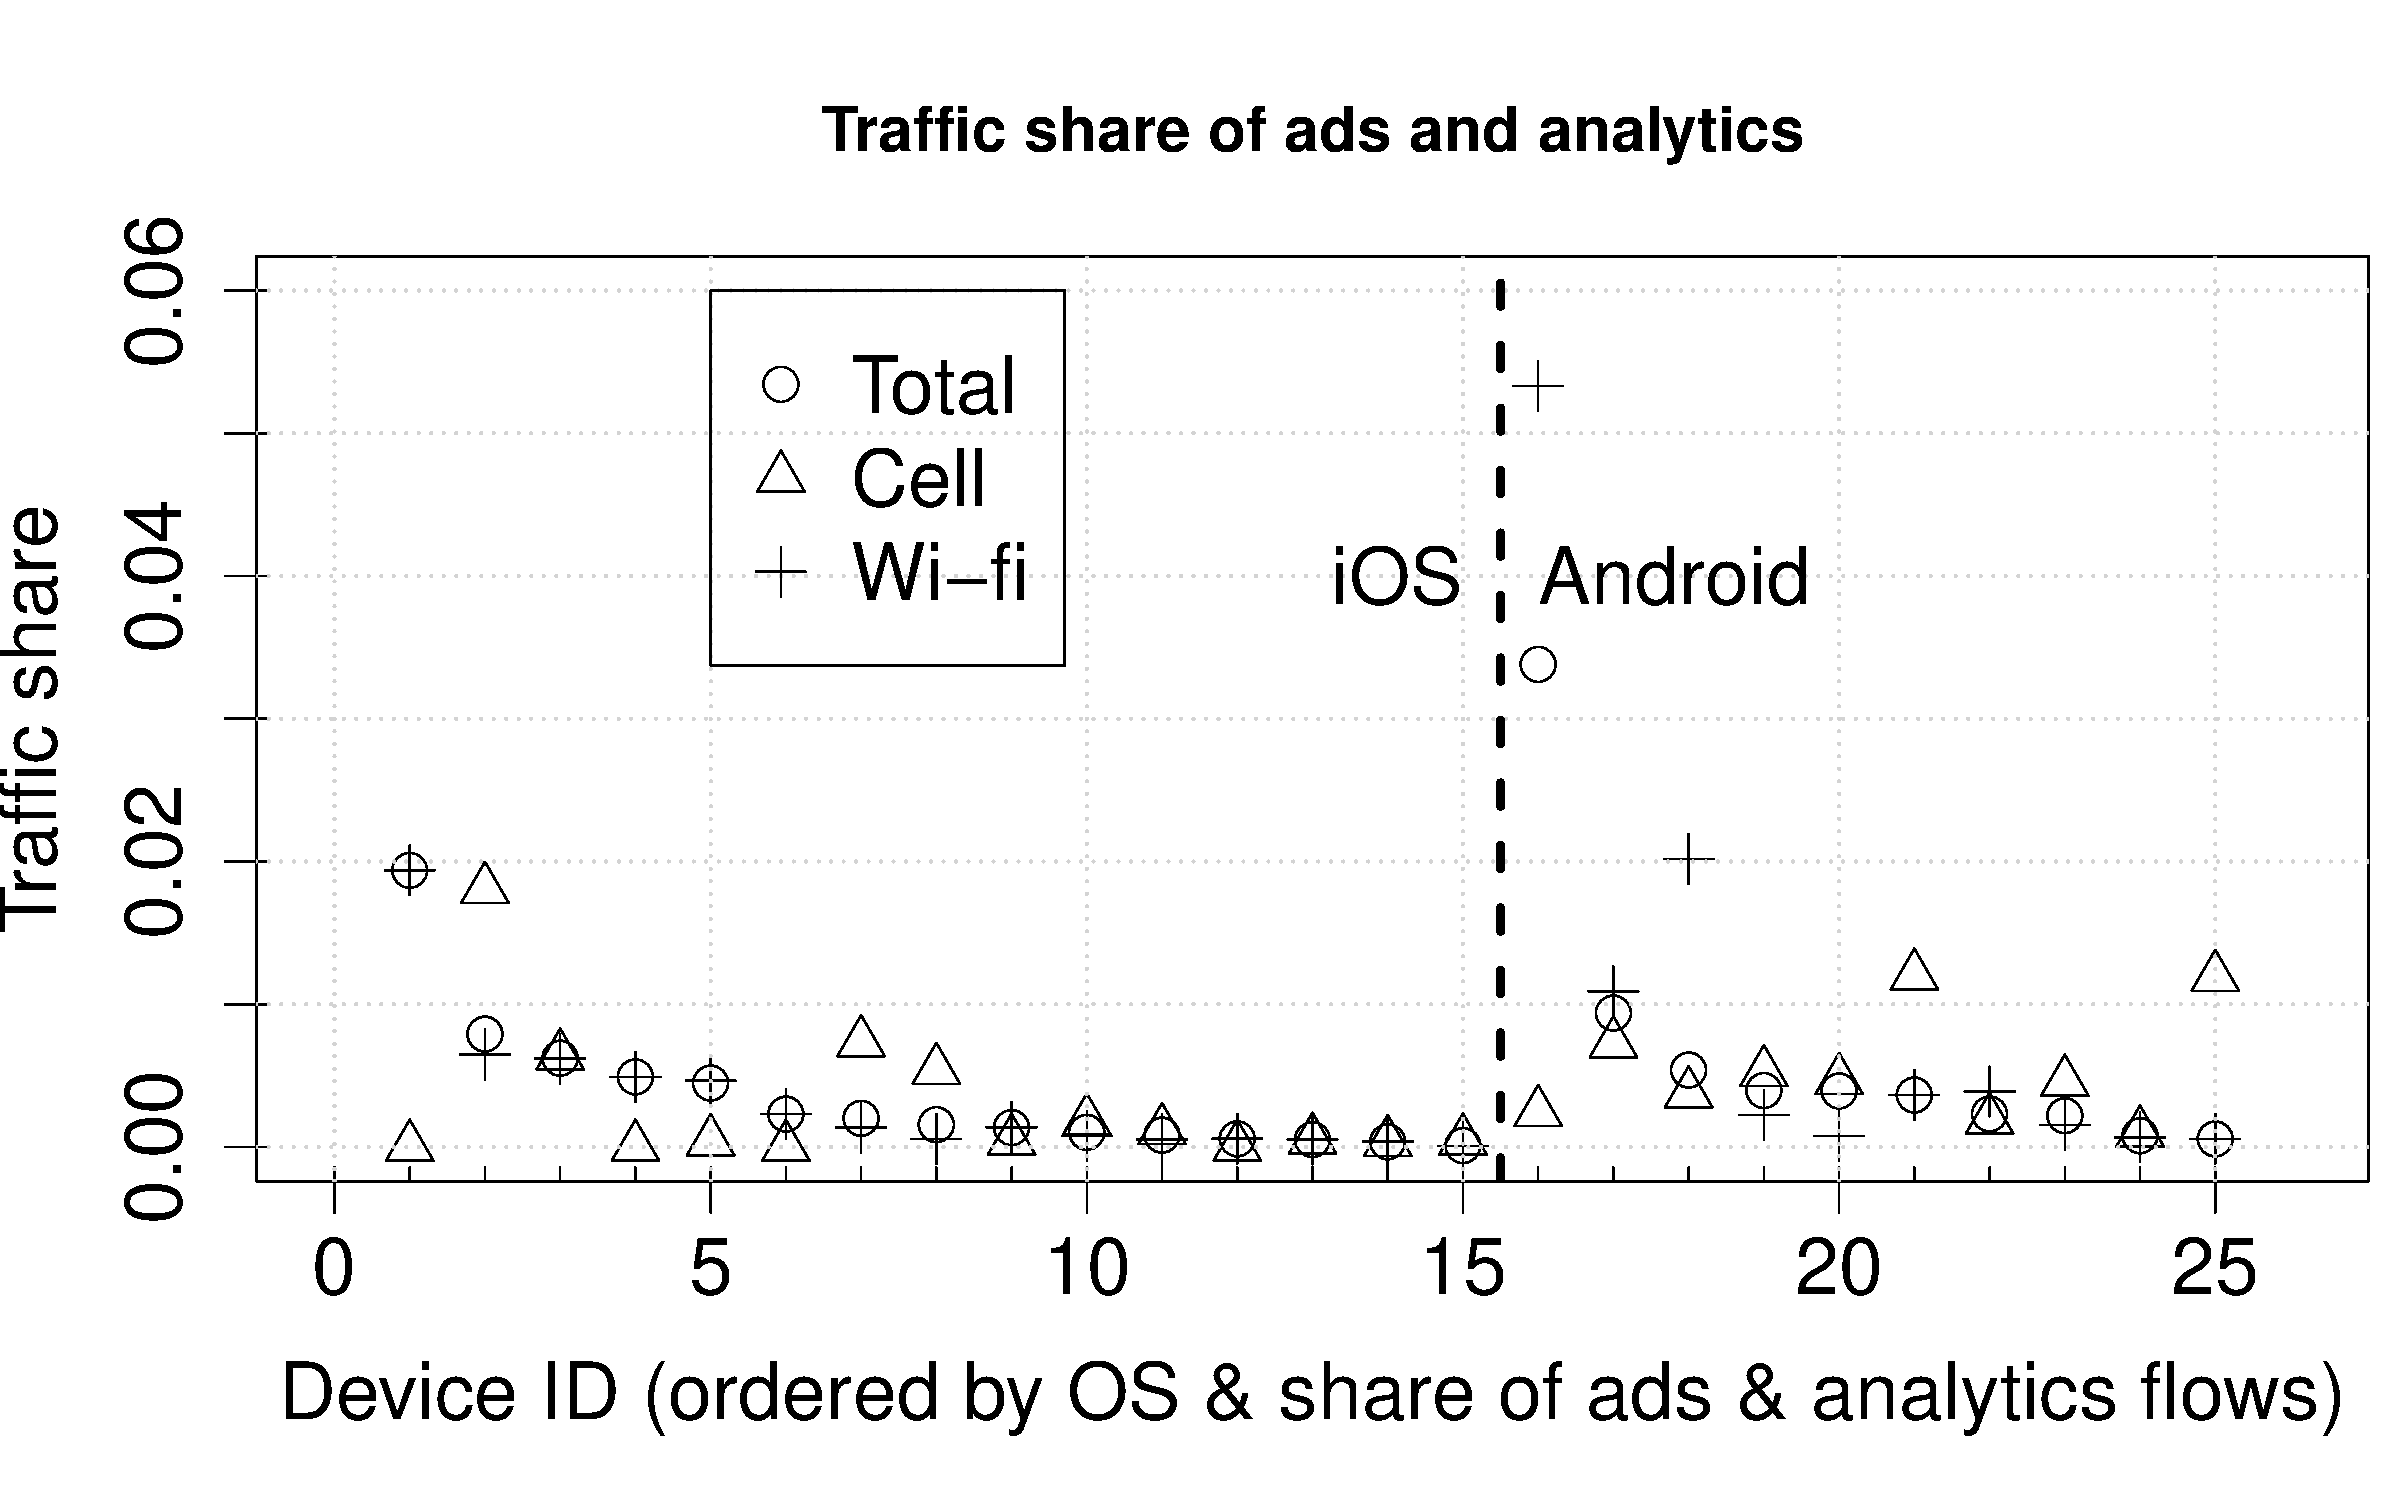
\includegraphics[width=\columnwidth]{plots/ad_share_bytes.pdf}
\caption{Fraction of traffic volume because of Ads and Analytics. \emph{\tbd{Check for id1 and id25}}}
\label{fig:description}
\end{figure}

\begin{figure}[t]
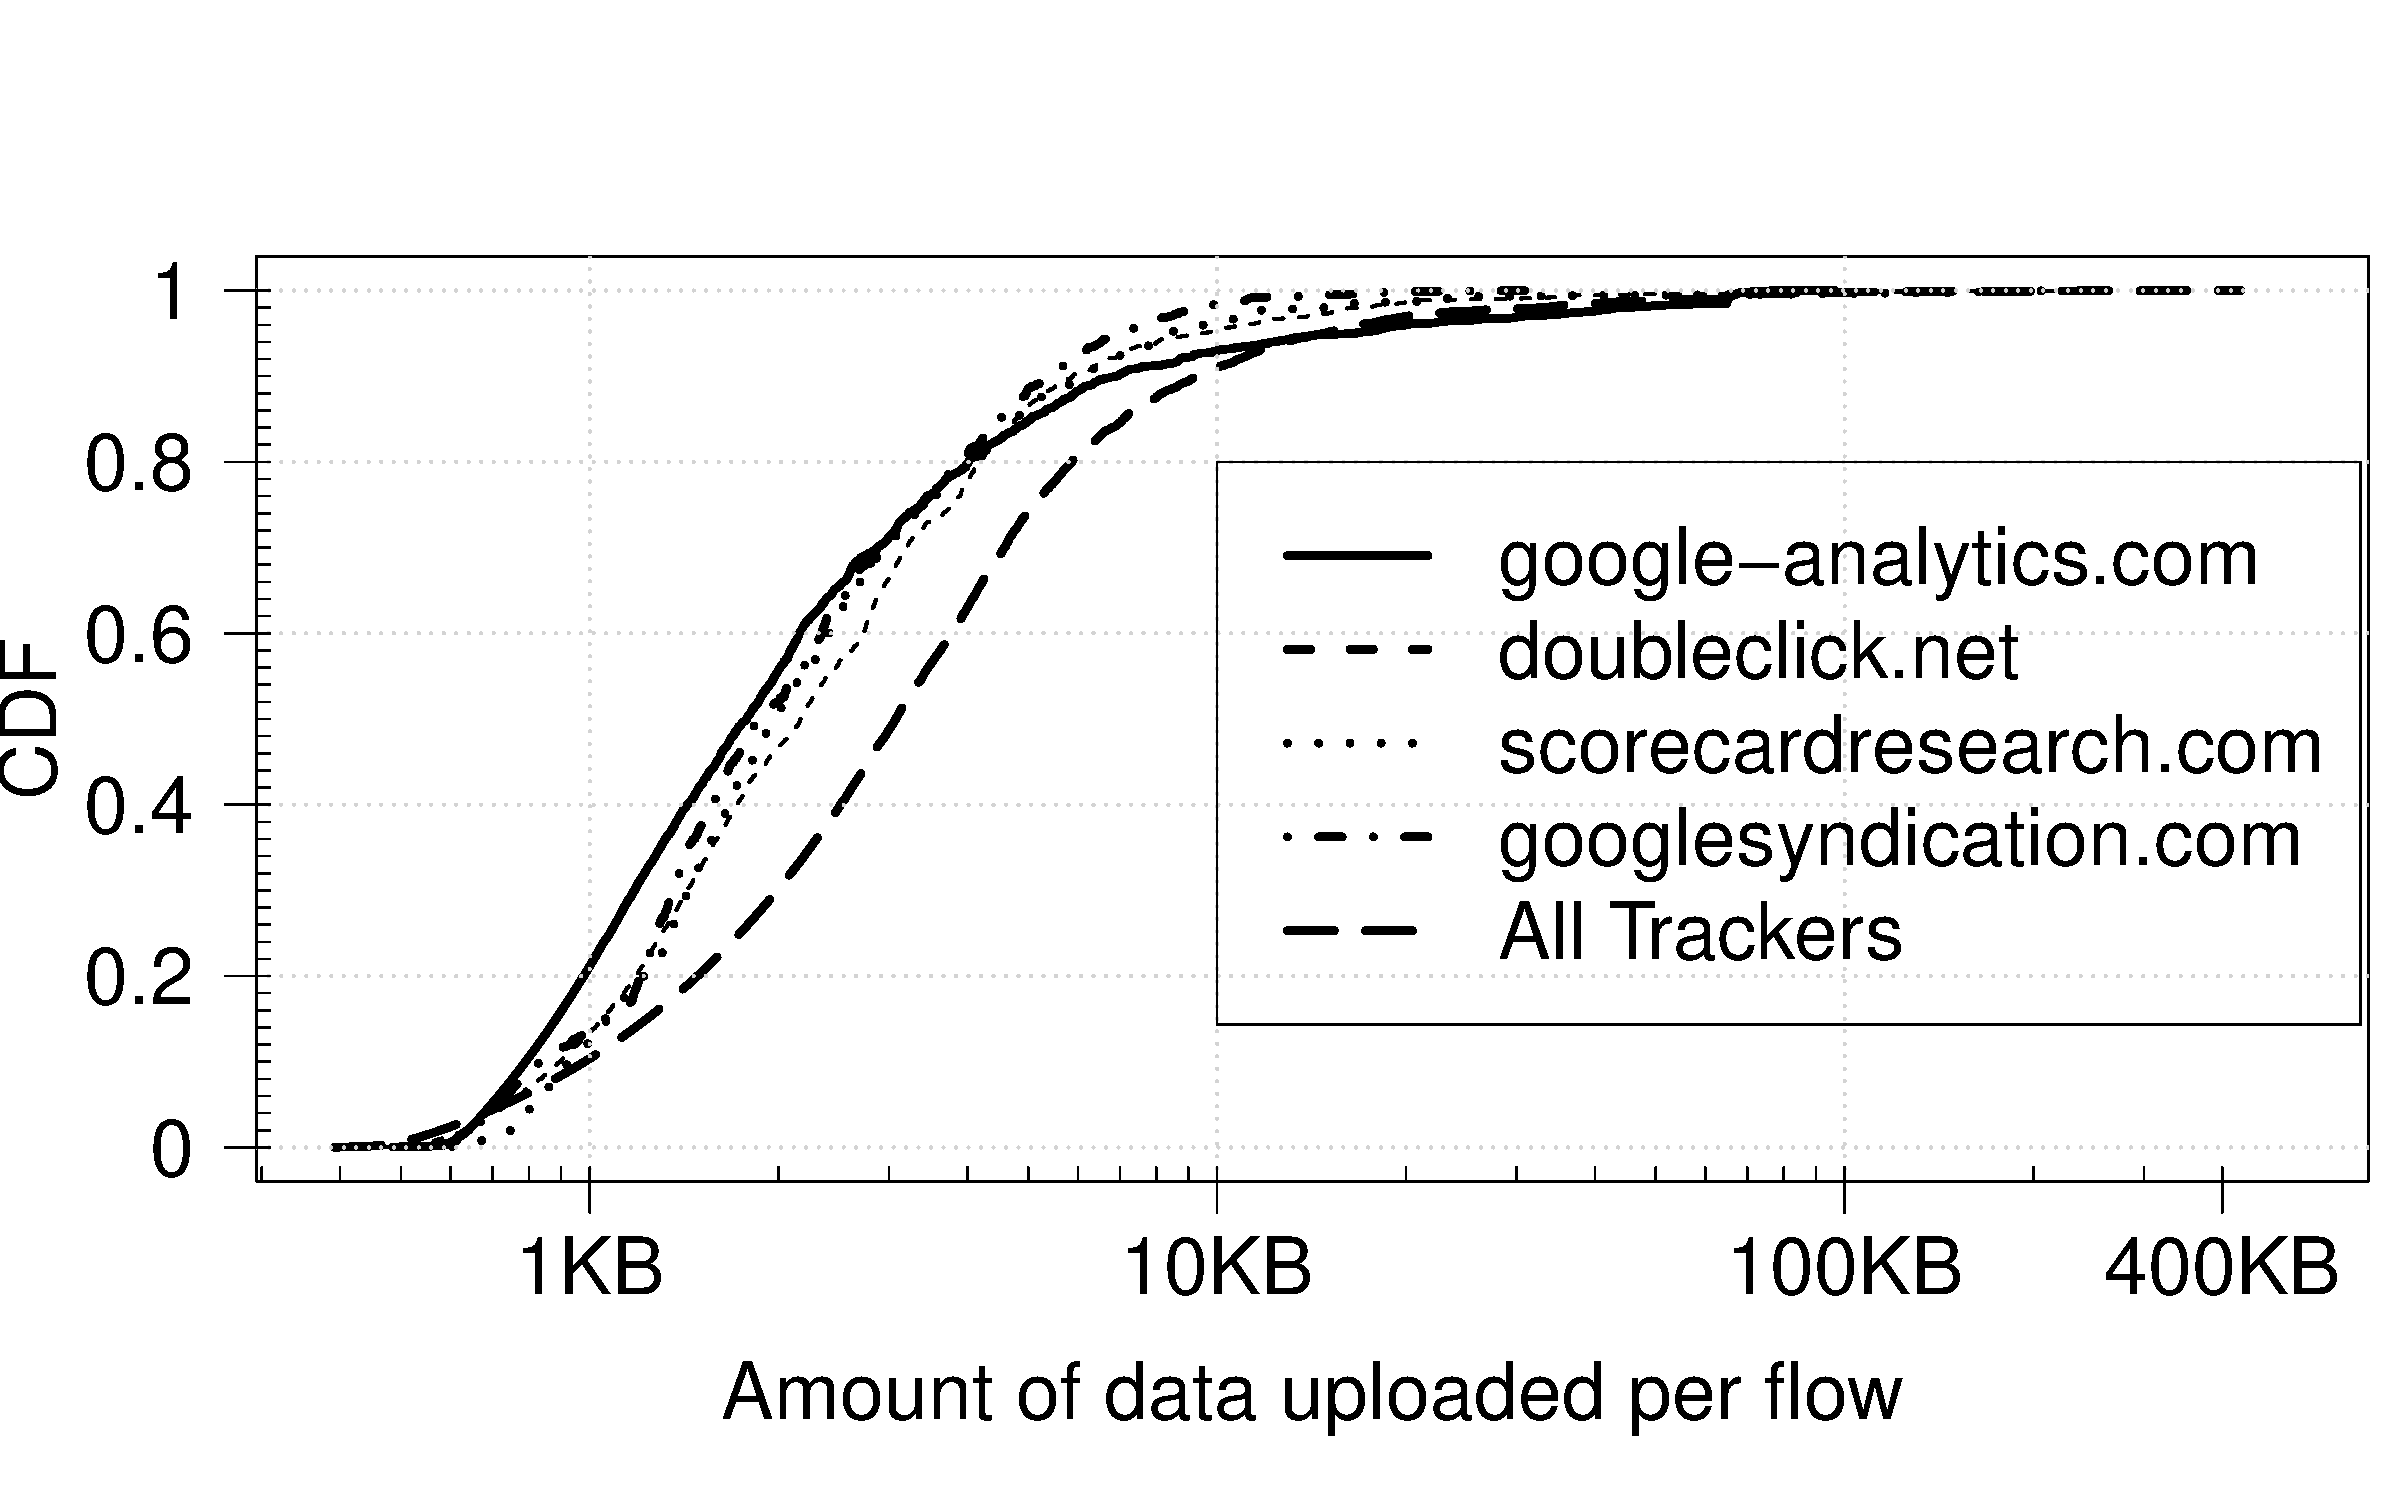
\includegraphics[width=\columnwidth]{plots/distrib_ad_uploads.pdf}
\caption{Distribution of bytes uploaded by ads and analytics sites. \emph{The distribution of bytes uploaded by all ads and analytics sites and the top four ads sites based on traffic volume across all users}.}
\label{fig:description}
\end{figure}

\begin{figure}[t]
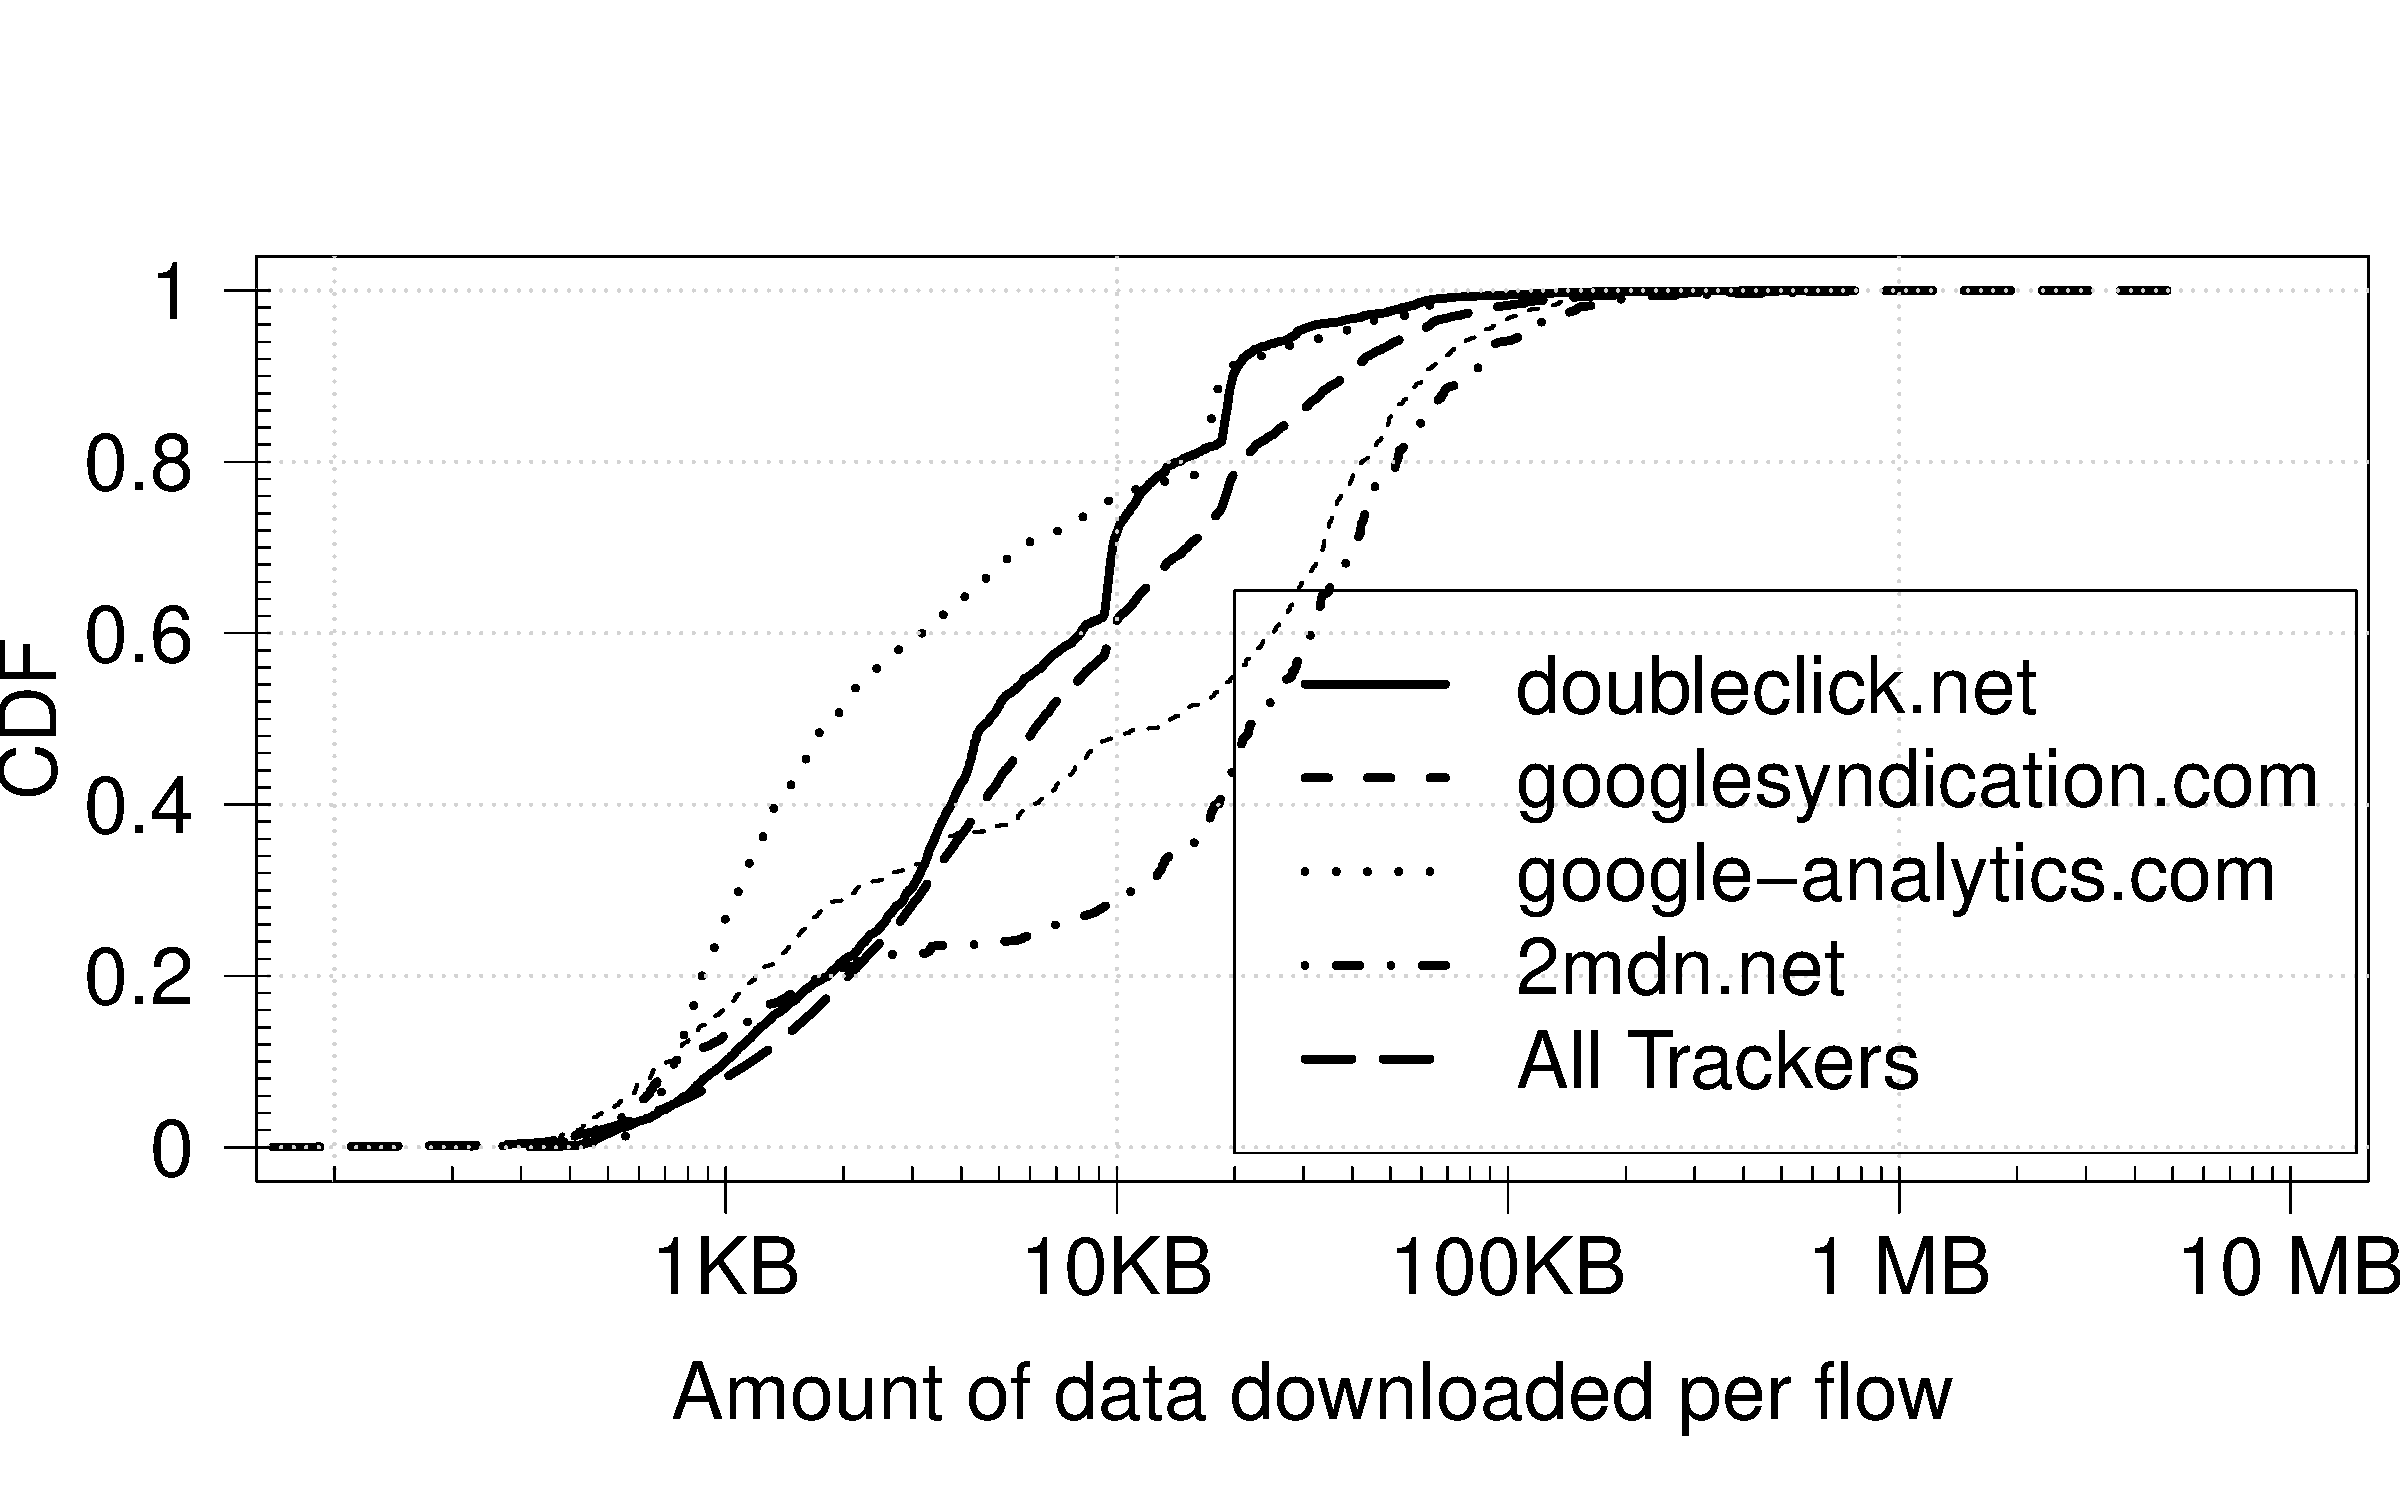
\includegraphics[width=\columnwidth]{plots/distrib_ad_downloads.pdf}
\caption{Distribution of bytes downloaded by ads and analytics sites. \emph{The distribution of bytes uploaded by all ads and analytics sites and the top four ads sites based on traffic volume across all users}.}
\label{fig:description}
\end{figure}

\begin{table}[t]
\centering
\begin{small}
\begin{tabular}{|p{0.35\columnwidth}|p{0.1\columnwidth}|p{0.15\columnwidth}|p{0.1\columnwidth}|}
\hline
\multirow{2}{*}{\bf Tracker} & \multicolumn{3}{c|}{\bf Number of devices tracked}\tabularnewline
\cline{2-4}
   &  {\bf Total} & {\bf Android} & {\bf iOS} \tabularnewline
\hline
doubleclick.net & 25 & 11 & 14 \tabularnewline
\hline
google-analytics.com   & 25 & 11 & 14 \tabularnewline
\hline
googlesyndication.com  & 22 & 10 & 12 \tabularnewline
\hline
admob.com  & 21 & 10 & 11 \tabularnewline
\hline
scorecardresearch.com &  21 & 10 & 11 \tabularnewline
\hline
2mdn.net  &  20 & 9 &  11 \tabularnewline
\hline
atdmt.com  & 18 & 9 &  9 \tabularnewline
\hline
imrworldwide.com & 18 &  9 &  9 \tabularnewline
\hline
flurry.com & 17 & 7 &  10 \tabularnewline
\hline
googleadservices.com  & 17 & 8 &  9 \tabularnewline
\hline
\end{tabular}
\end{small}
\caption{The top 10 ads and analytics sites that tracked the devices in our dataset.
\emph{Two trackers, \emph{doubleclick.net} and\emph{google-analytics.com}, were tracking all the 25 devices in our dataset.}}
\label{tab:top_trackers}
\end{table}


\begin{table*}[t]
    \begin{tabular}{l|l|l|l|l|l|l|l|l|l|l}
       Dataset&Platform&Proto&\# Apps&Email&Location&Username&Password&Android ID&Contacts&IMEI\\
       \hline
       Google Play&Android&HTTP&100&?&10 (10\%)&7 (7\%)&1 (1\%)&21 (21\%)&0 (0\%)&13 (13\%)\\
       \hline
       Third Party&Android&HTTP&908&?&32 (3.5\%)&?&0 (0\%)&95 (10.4\%)&4 (0.4\%)&48 (5.3\%)\\
       \hline
       App Store&iPhone&HTTP&100&?&?&?&?&?&?&?\\
    \end{tabular}
    \caption{\label{tbl:pii}Summary of personally identifiable information leaked in plaintext (HTTP) by Android and iPhone apps.}
  \end{table*}
  

  {\bf Android Apps.}
  When we inspect the data from our controlled study, we see that some apps contact a large number of external servers while others contact significantly fewer.
  In Figure~\ref{fig:android-cdns}, we show both the total number of servers contacted (solid lines) as well as the number of organizations contacted (dotted lines) for both the top-100 Google Play dataset and the top-2000 third-party dataset.
  To quantify ``organizations contacted'', we performed whois lookups on all servers contacted and mapped them to an organization name, allowing us to tighten our upper bound on the number of companies/entities able to track the user through a single app.
  Returning to the figure, we see...~\ref{fig:android-cdns}...\tbd{Amy...}


  {\bf iPhone Apps.}
  \tbd{Shen...}

\subsection{Personally Identifiable Information}
 
  Finally, we turn to information leaked by individual applications. We do not report on data leaked for our real users here, but only the data leaked by our controlled apps in isolation.
  We created fake user accounts on the test phones for a fake user named ``Tess Droid'', with fake contact information and fake Twitter and Facebook accounts. 
  We were then able to check that none of this data ever was released over the network, either in plaintext (HTTP) or encrypted (HTTPS, see \S\ref{sec:bumping}).
  
  We consider data to be `leaked' when any personally identifiable information -- email address, phone number, IMEI number -- is sent across the network under HTTP or HTTPS.
  Some of this information may be relevant to the app -- \eg{}, many apps legitimately require email access. 
  However, none of this information should ever travel across the network in plaintext (HTTP), which we see violated in serveral cases.

  In Table~\ref{tbl:pii}, we see the type of PII leaked for both Android and iPhone apps.
  For Android apps, IMEI and Android ID are the most commonly leaked forms of PII in both the Google Play and third-party dataset.
  Although not popularly thought of as ``private'' data, each of these identifiers are globally unique: IMEI is a unique identifier tied to a phone, and an Android ID is an identifier tied to a user's Google Account, used across many services on the Internet. 
  Consequently, either of these datapoints can be used to track or correlate a user's behavior across all sites the user visits that sell or collaborate with tracking data: a user's behavior on one site can easily be linked to their behavior on any other site they visit.
  With Android ID being tracked by between 10 and 20\% of apps in our study, and IMEI being tracked by between 5\% and 13\% of apps in our study, this suggests that global user tracking across collaborating services can be easily achieved today just by using this identifier.
  \tbd{...}

  Other informaiton like contacts, email, and passwords were rarely leaked in the clear, but all were leaked on occaision, suggesting that stricter monitoring of Android app behavior is needed -- contrastingly, no iPhone apps (which are manually given clearance by Apple before hitting the iPhone store) leaked passwords in plaintext~\tbd{is this true.}

  Moving to iPhone apps, \tbd{...}
%\subsection{Characterize Facebook Applications}

%Why Facebook was chosen?

%What do we observe ?

%What do we see in the User Agent Fields. 




\section{Behavior of Networks}

\subsubsection{Controlled Experiments}

\subsubsection{In the Wild}

We ignore connections from the same network and ISP in which our servers were placed.


\begin{figure}[t]
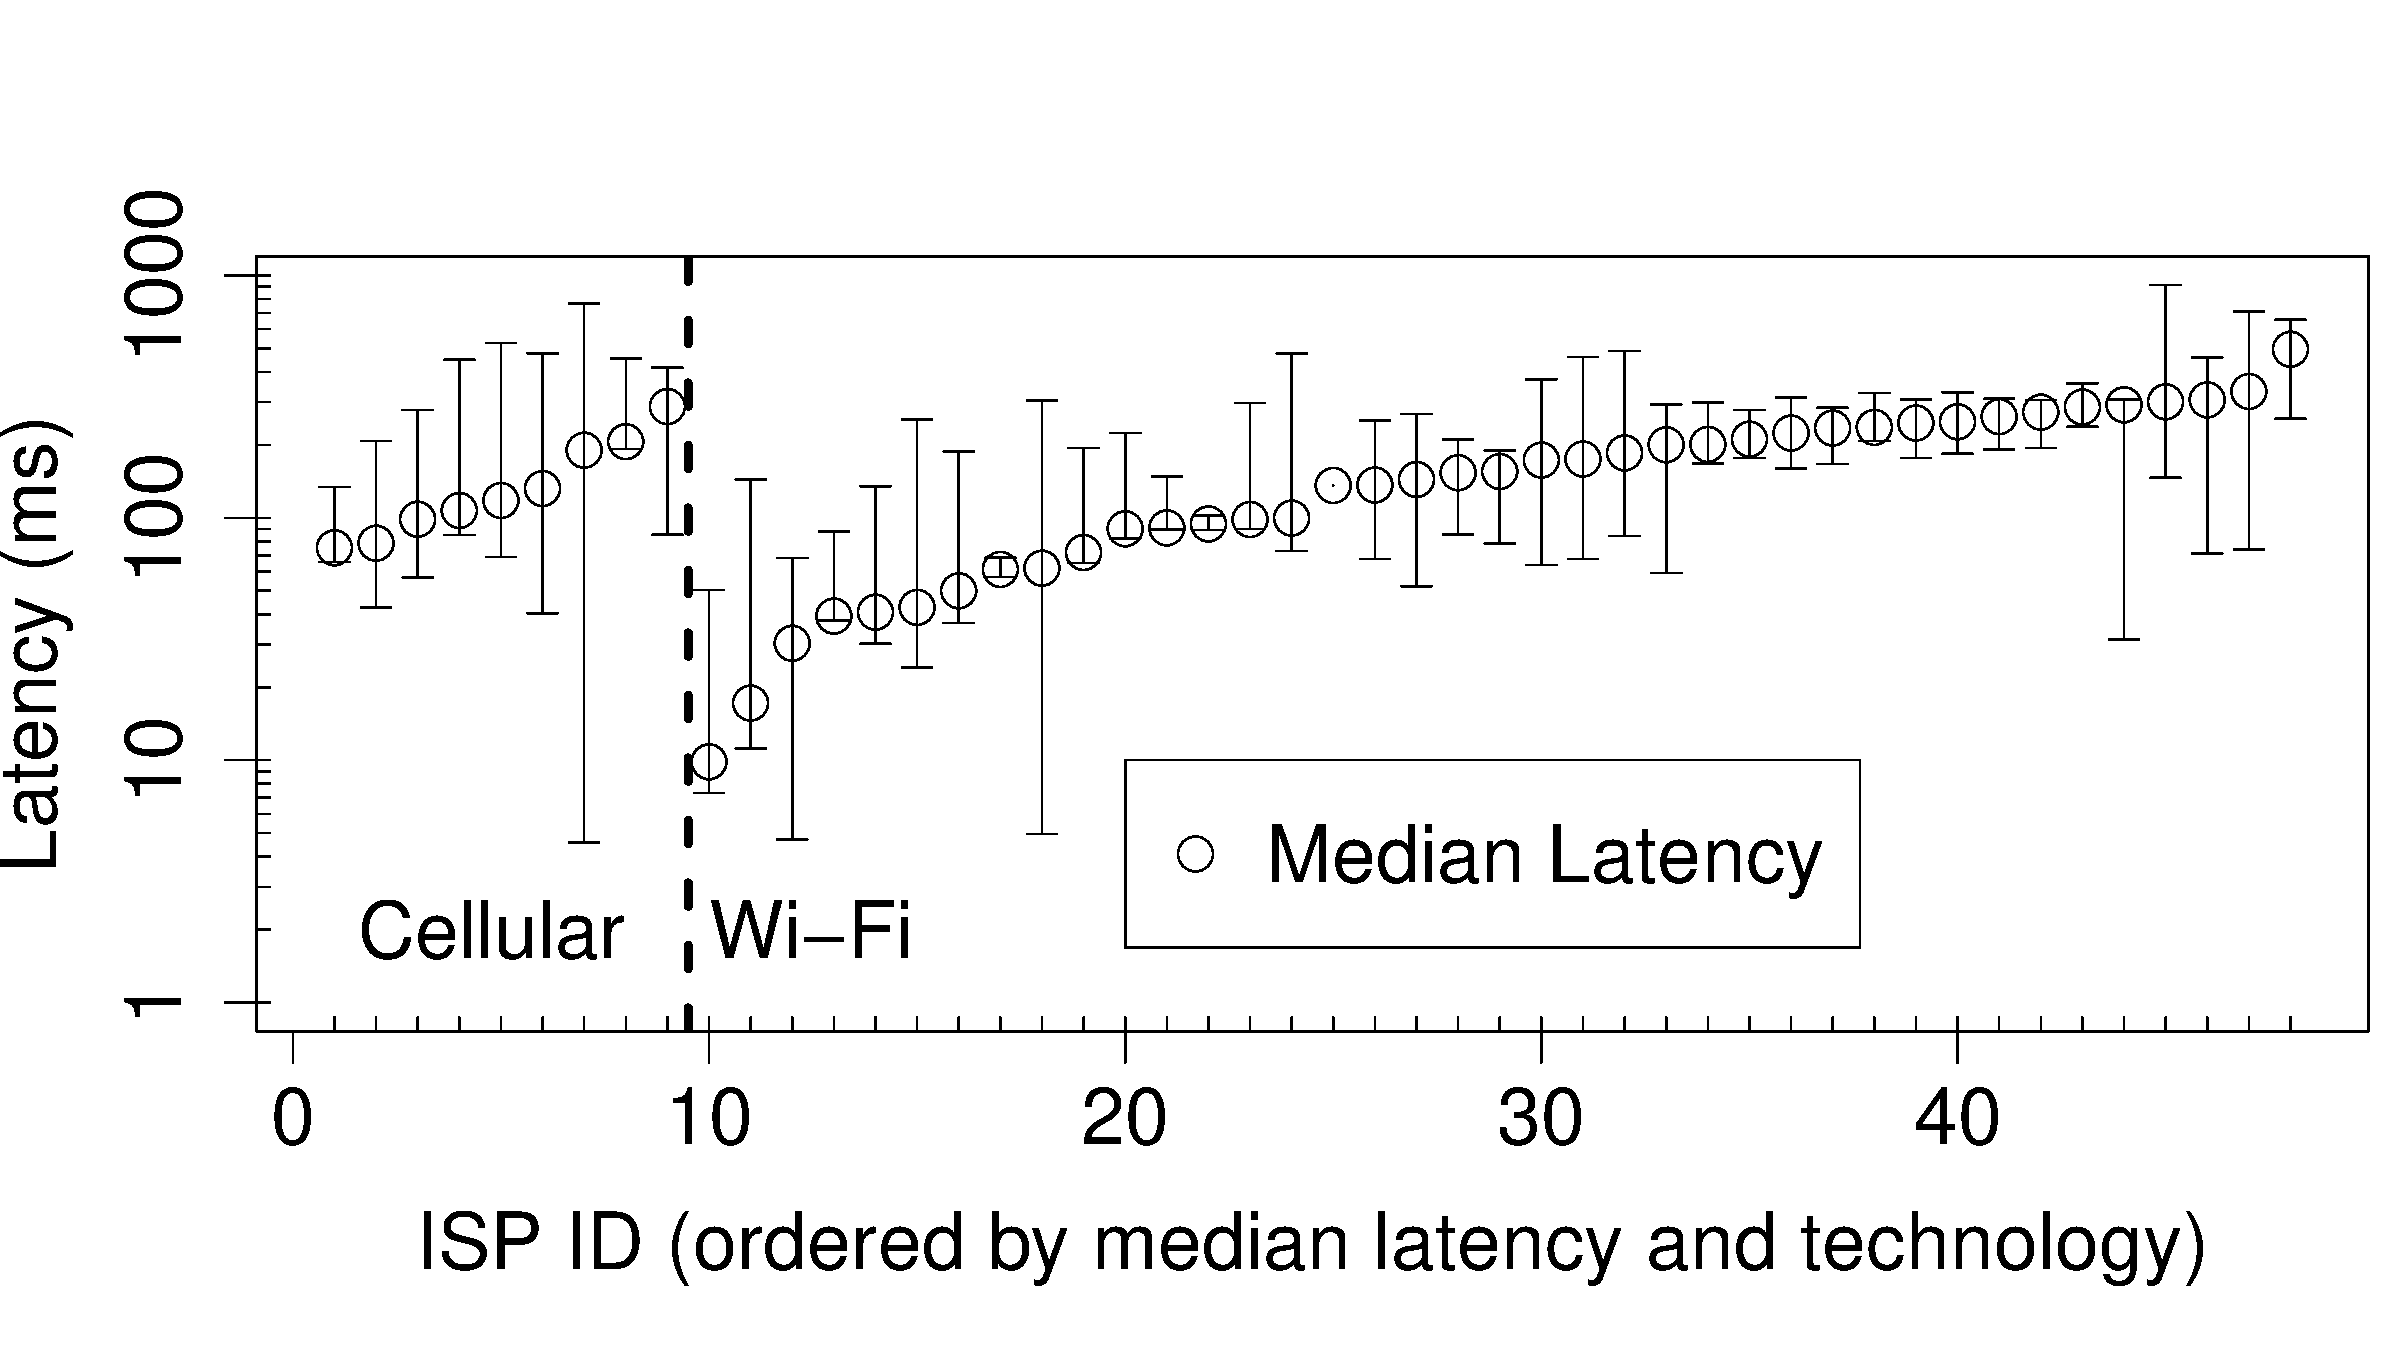
\includegraphics[width=\columnwidth]{plots/latency_isp_whisker.pdf}
\caption{One-way latency from VPN server to mobile devices. \emph{Connections from cellular ISPs suffer a higher delay compared to Wi-Fi ISPs. The delays from Cellular ISPs is comparable to connecting from a Wi-Fi ISP in another country. Error bars indicate the 91st and 9th percentile}.}
\label{fig:latency-across-isps}
\end{figure}


\begin{figure}[t]
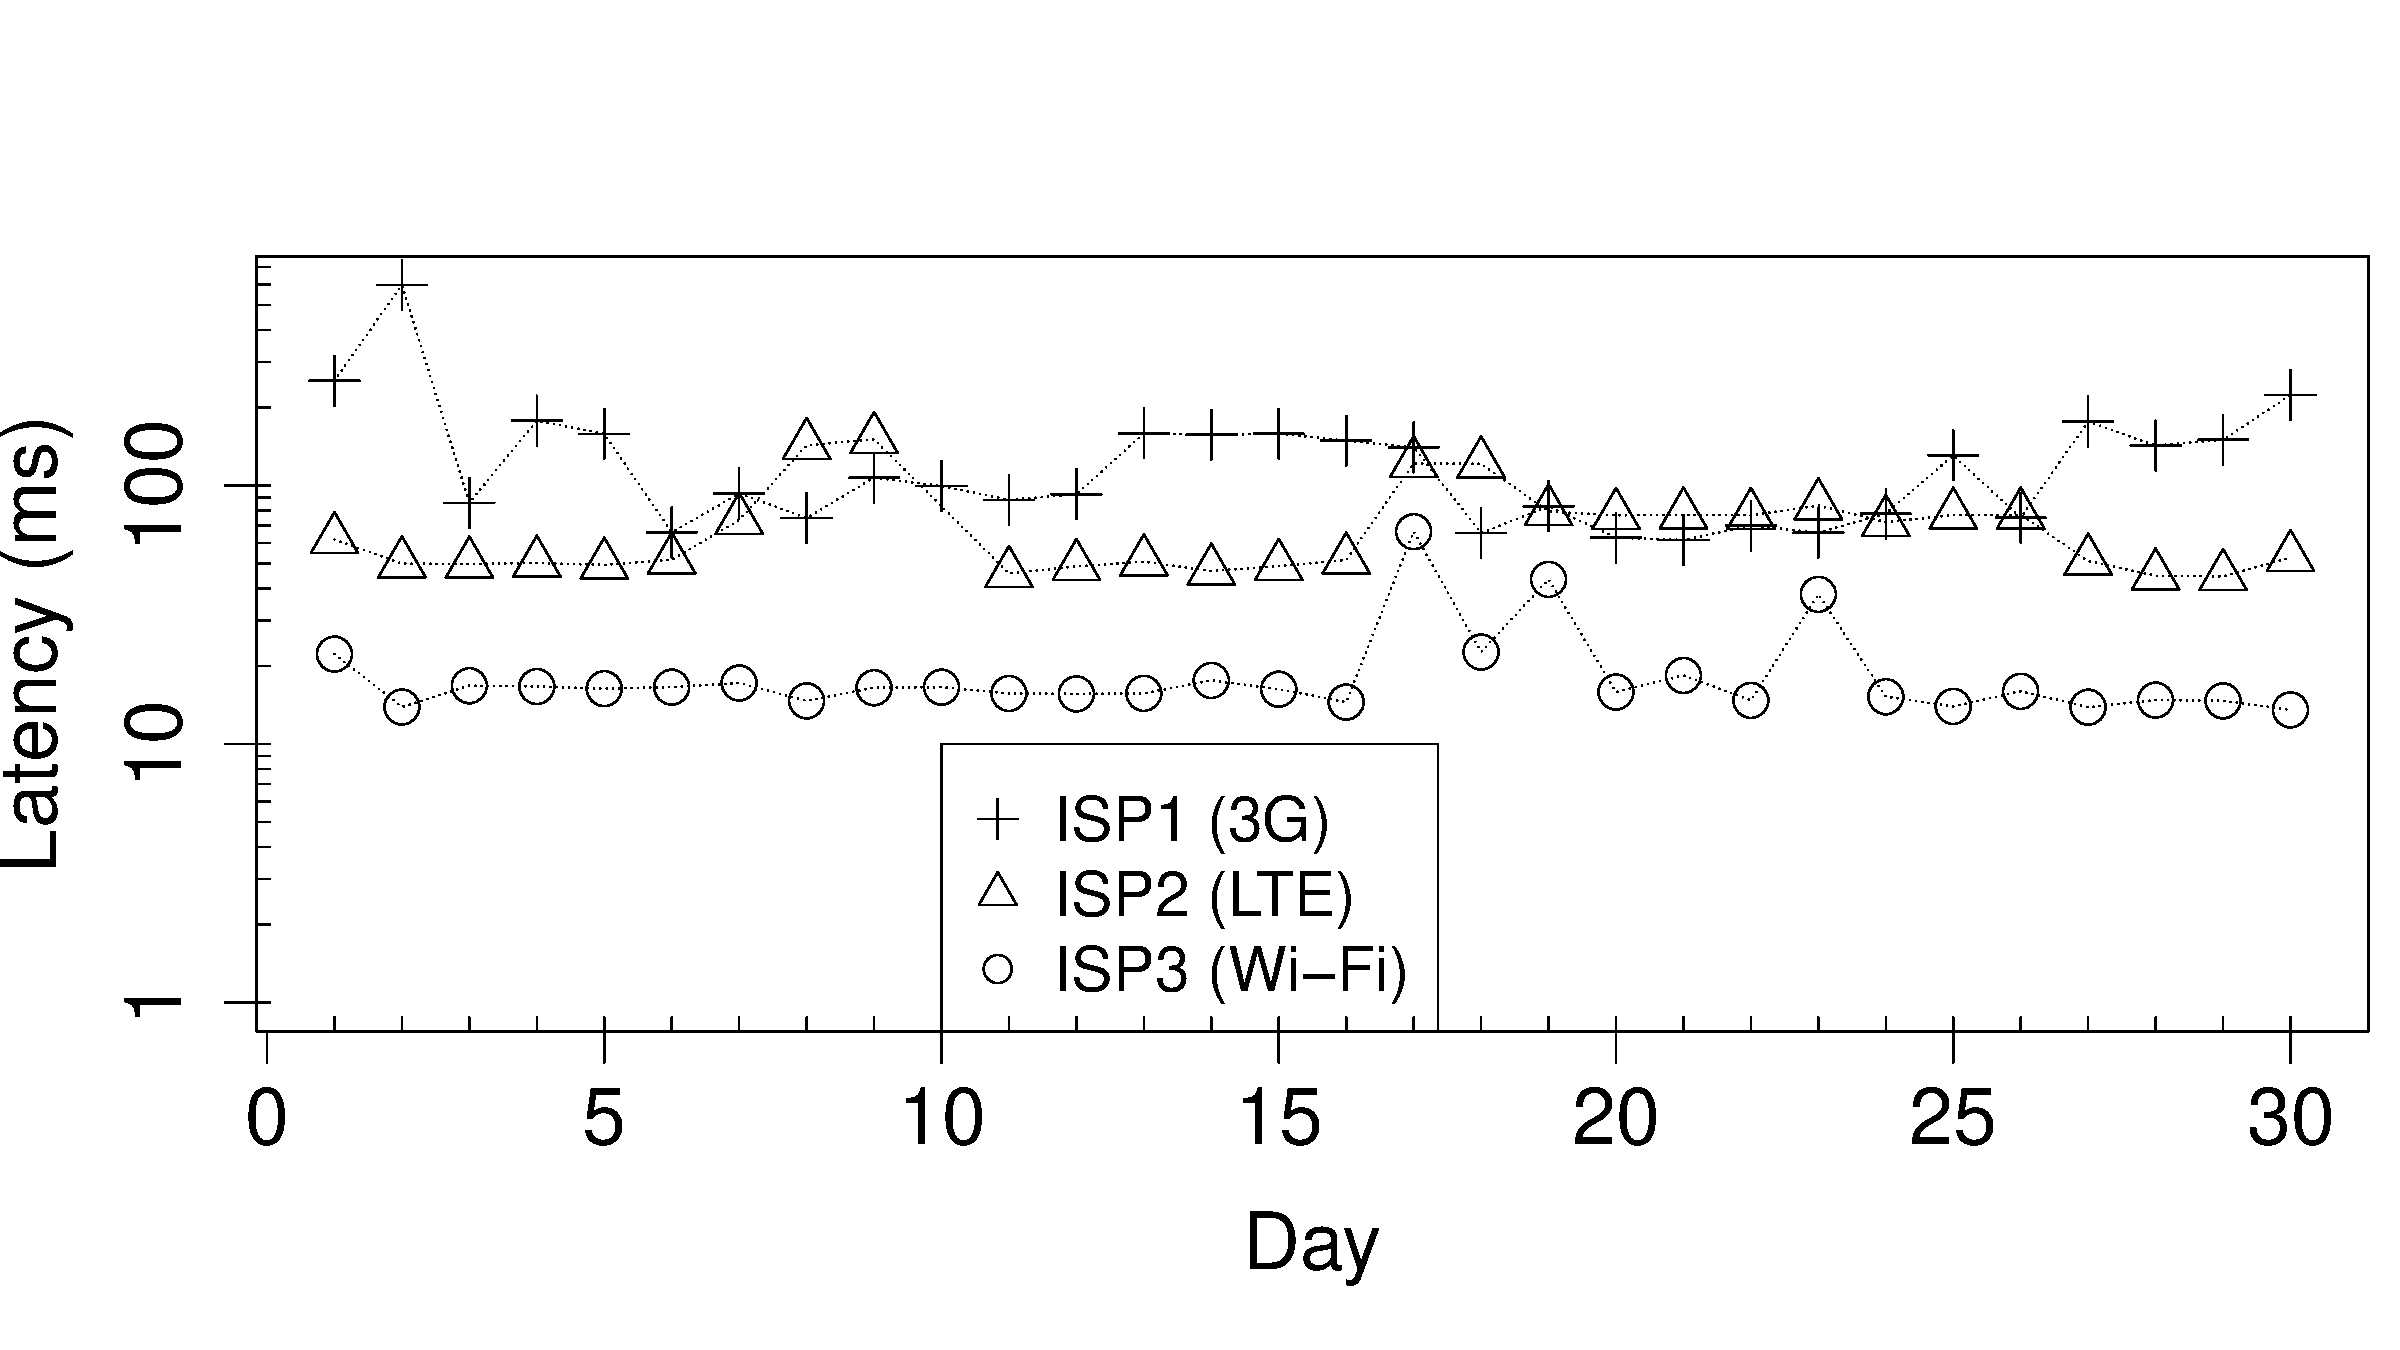
\includegraphics[width=\columnwidth]{plots/compare_isp_latency.pdf}
\caption{Comparison of ISPs that serve the same user during a 30 day time period. \emph{The LTE service provider has a smaller latency to the 3G provider. The smallest latency is observed by in the home Wi-Fi network.}}
\label{fig:compare-isp-latency}
\end{figure}

\begin{figure}[t]
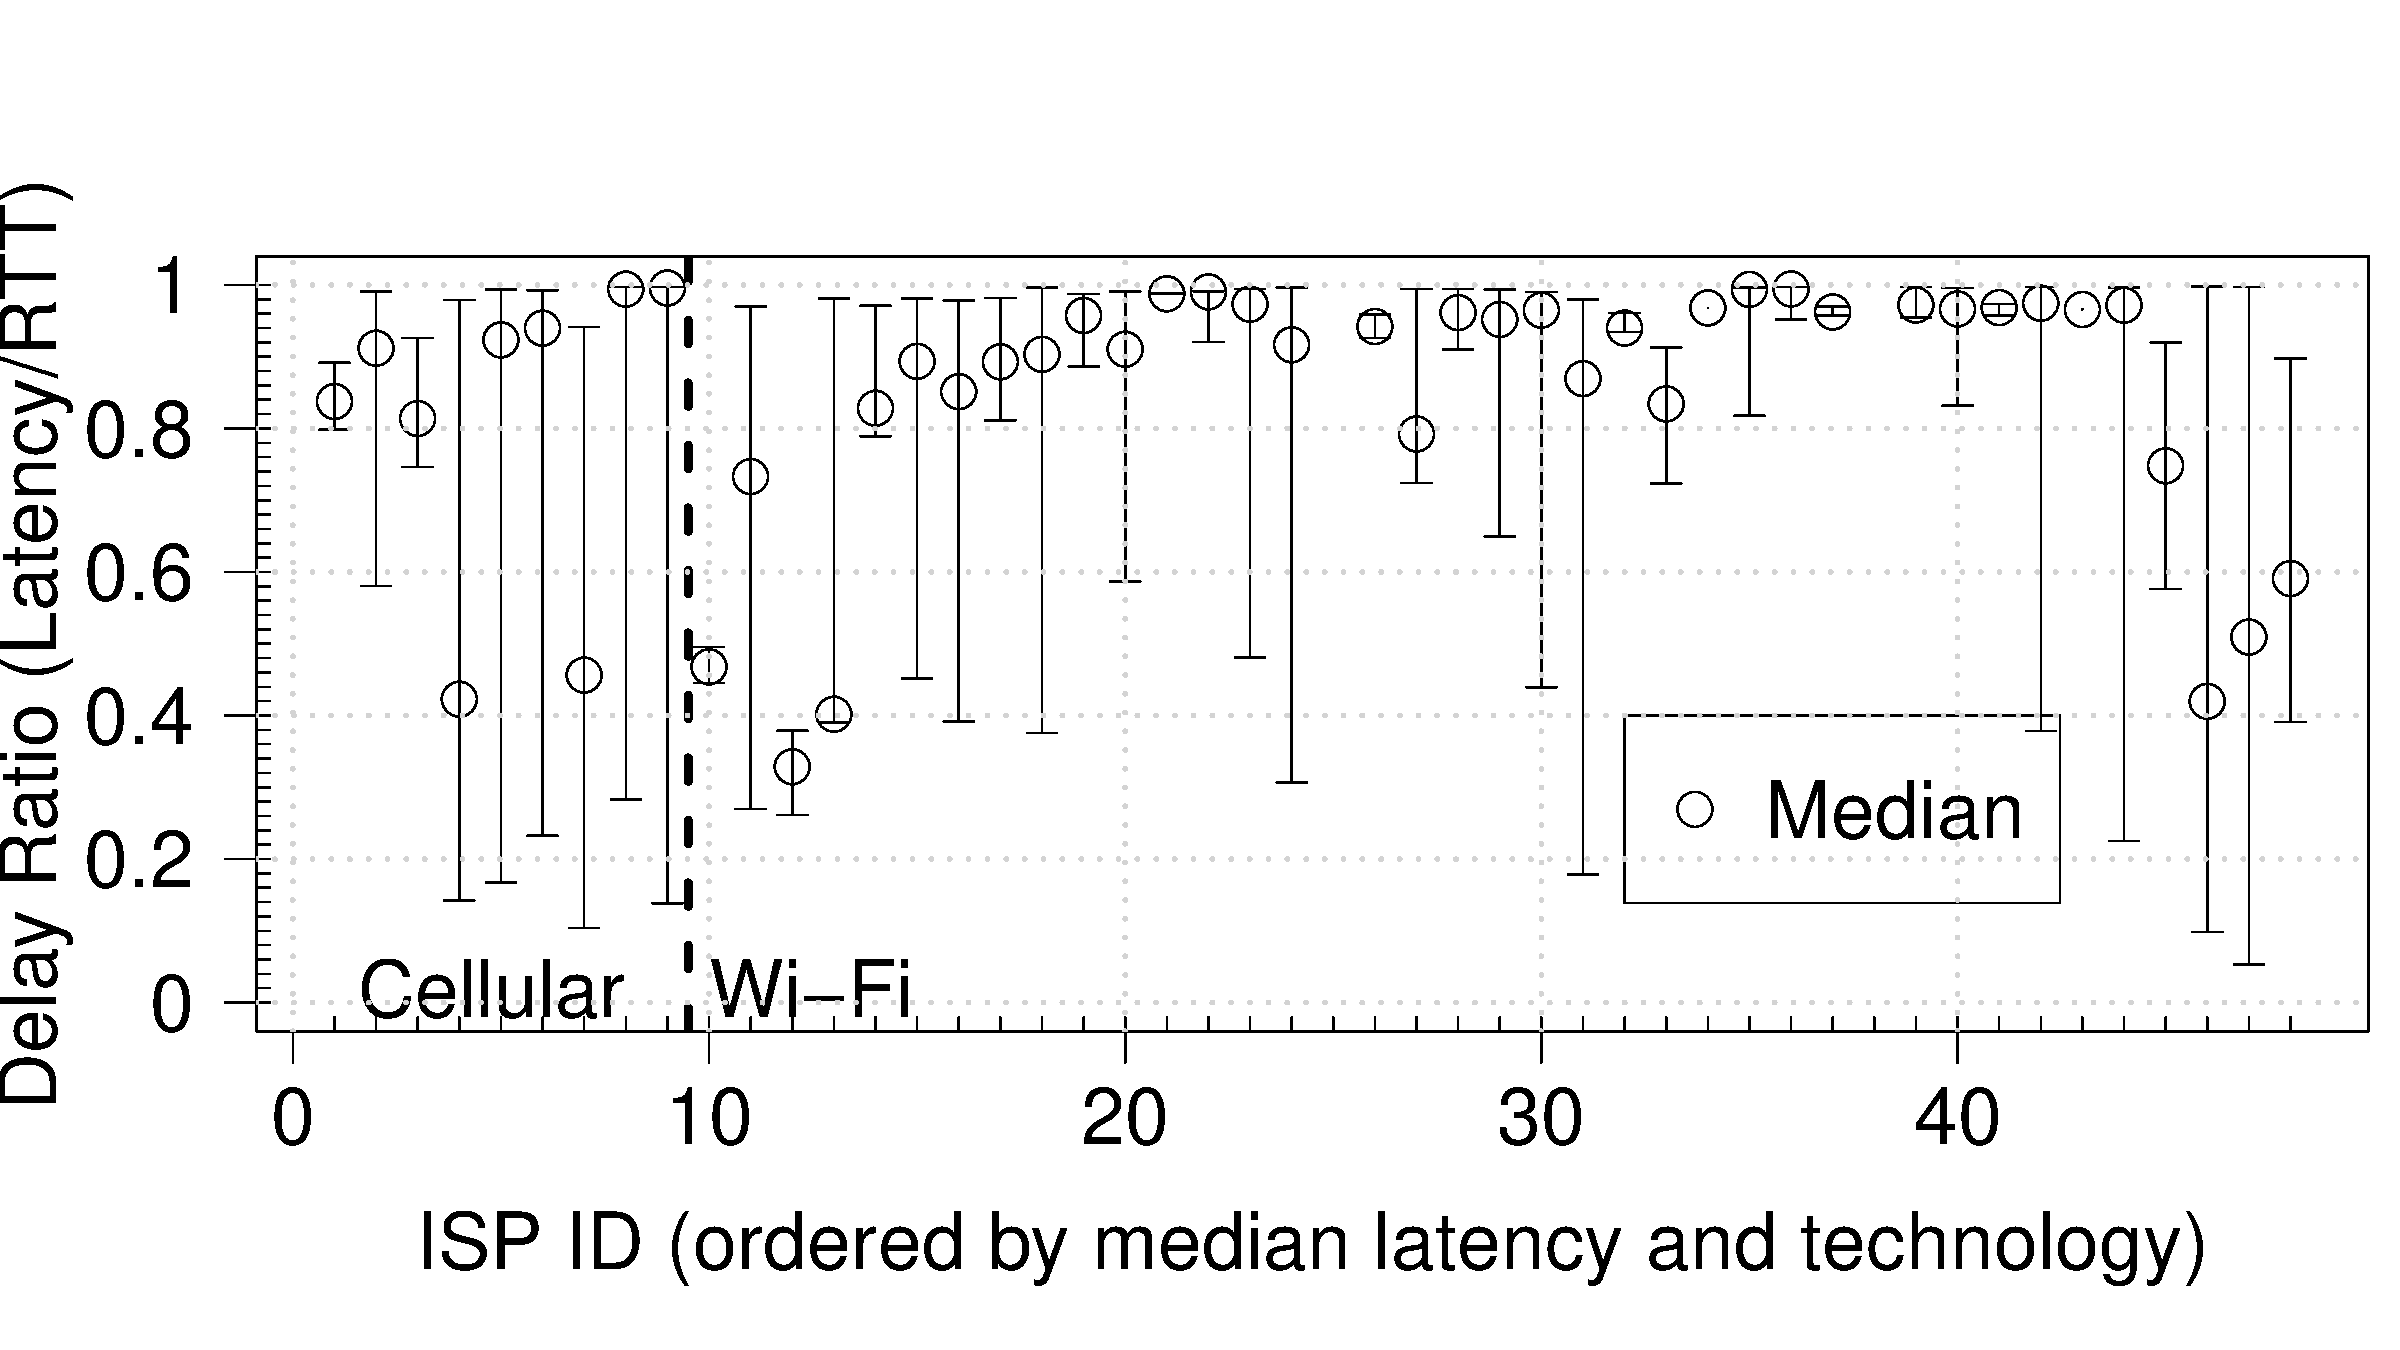
\includegraphics[width=\columnwidth]{plots/delay_ratio_isp_whisker.pdf}
\caption{Latency as a fraction of the round trip time to contact google services. \emph{In 35 ISPs of the 48 ISPs we observe that the latency of the mobile device to our server accounts for more than 90\% of the end-to-end round trip time. Error bars indicate the 91st and 9th percentile.}}
\label{fig:compare-delay-ratio}
\end{figure}

\begin{figure}[t]
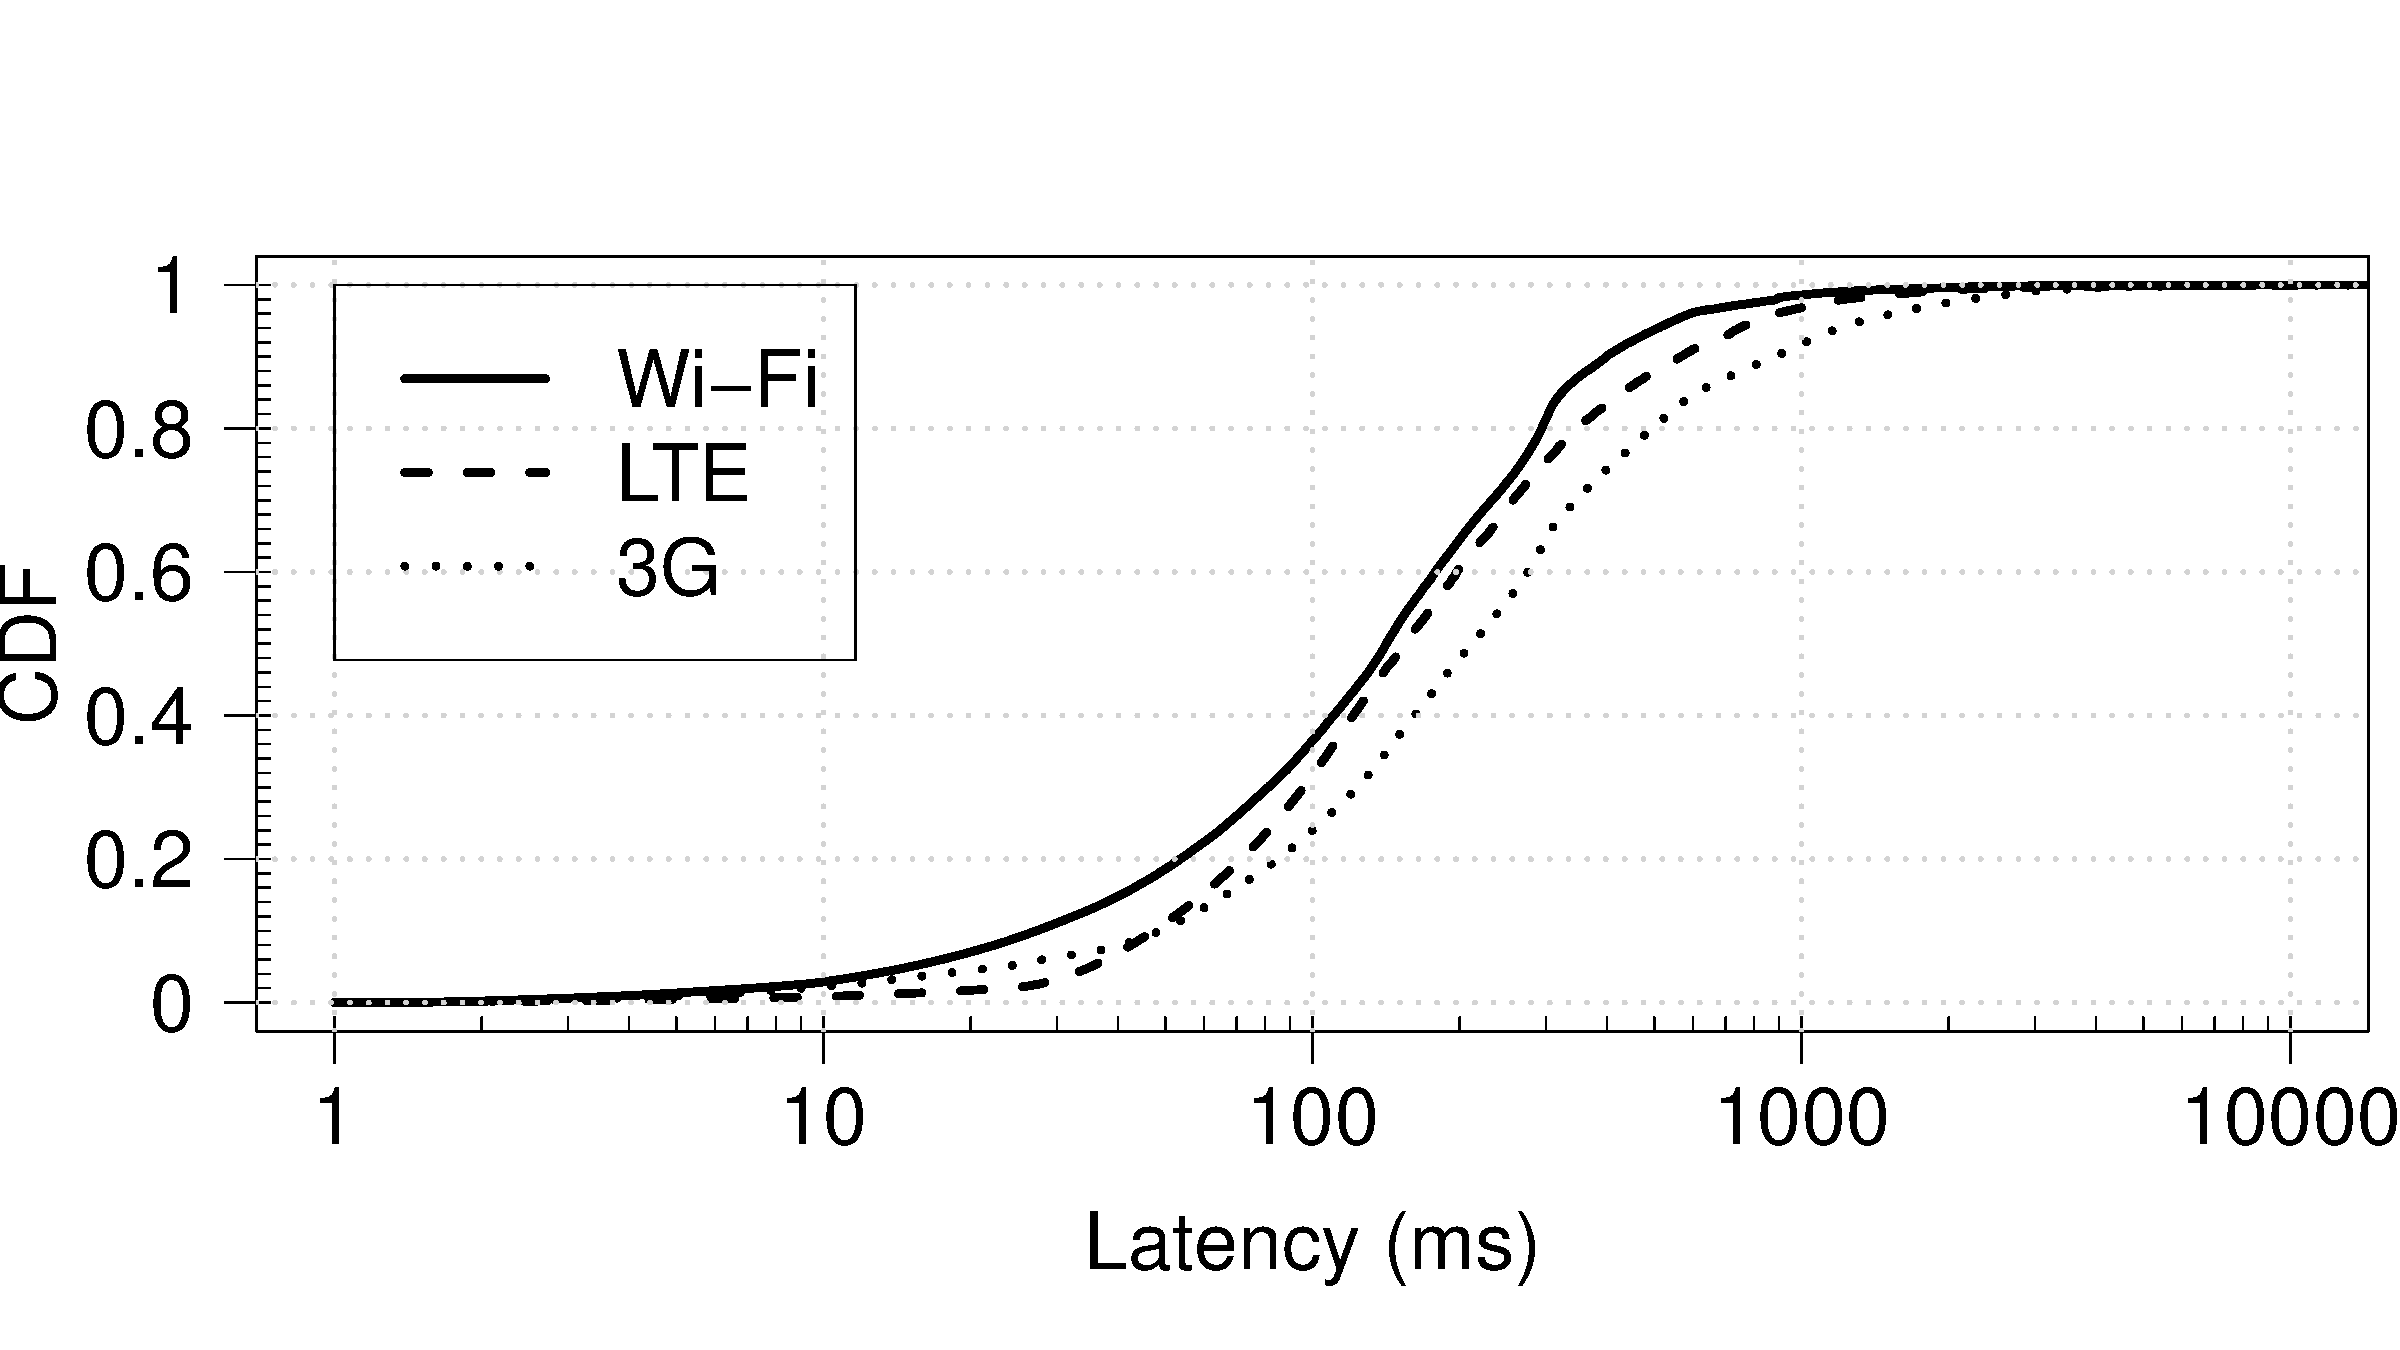
\includegraphics[width=\columnwidth]{plots/distrib_latency_technology.pdf}
\caption{Distribution of latency over cellular and \wifi ISPs. \emph{The distribution of latency observed when using LTE in the wild is similar to that observed for \wifi}.}
\label{fig:compare-delay-ratio}
\end{figure}

\begin{figure}[t]
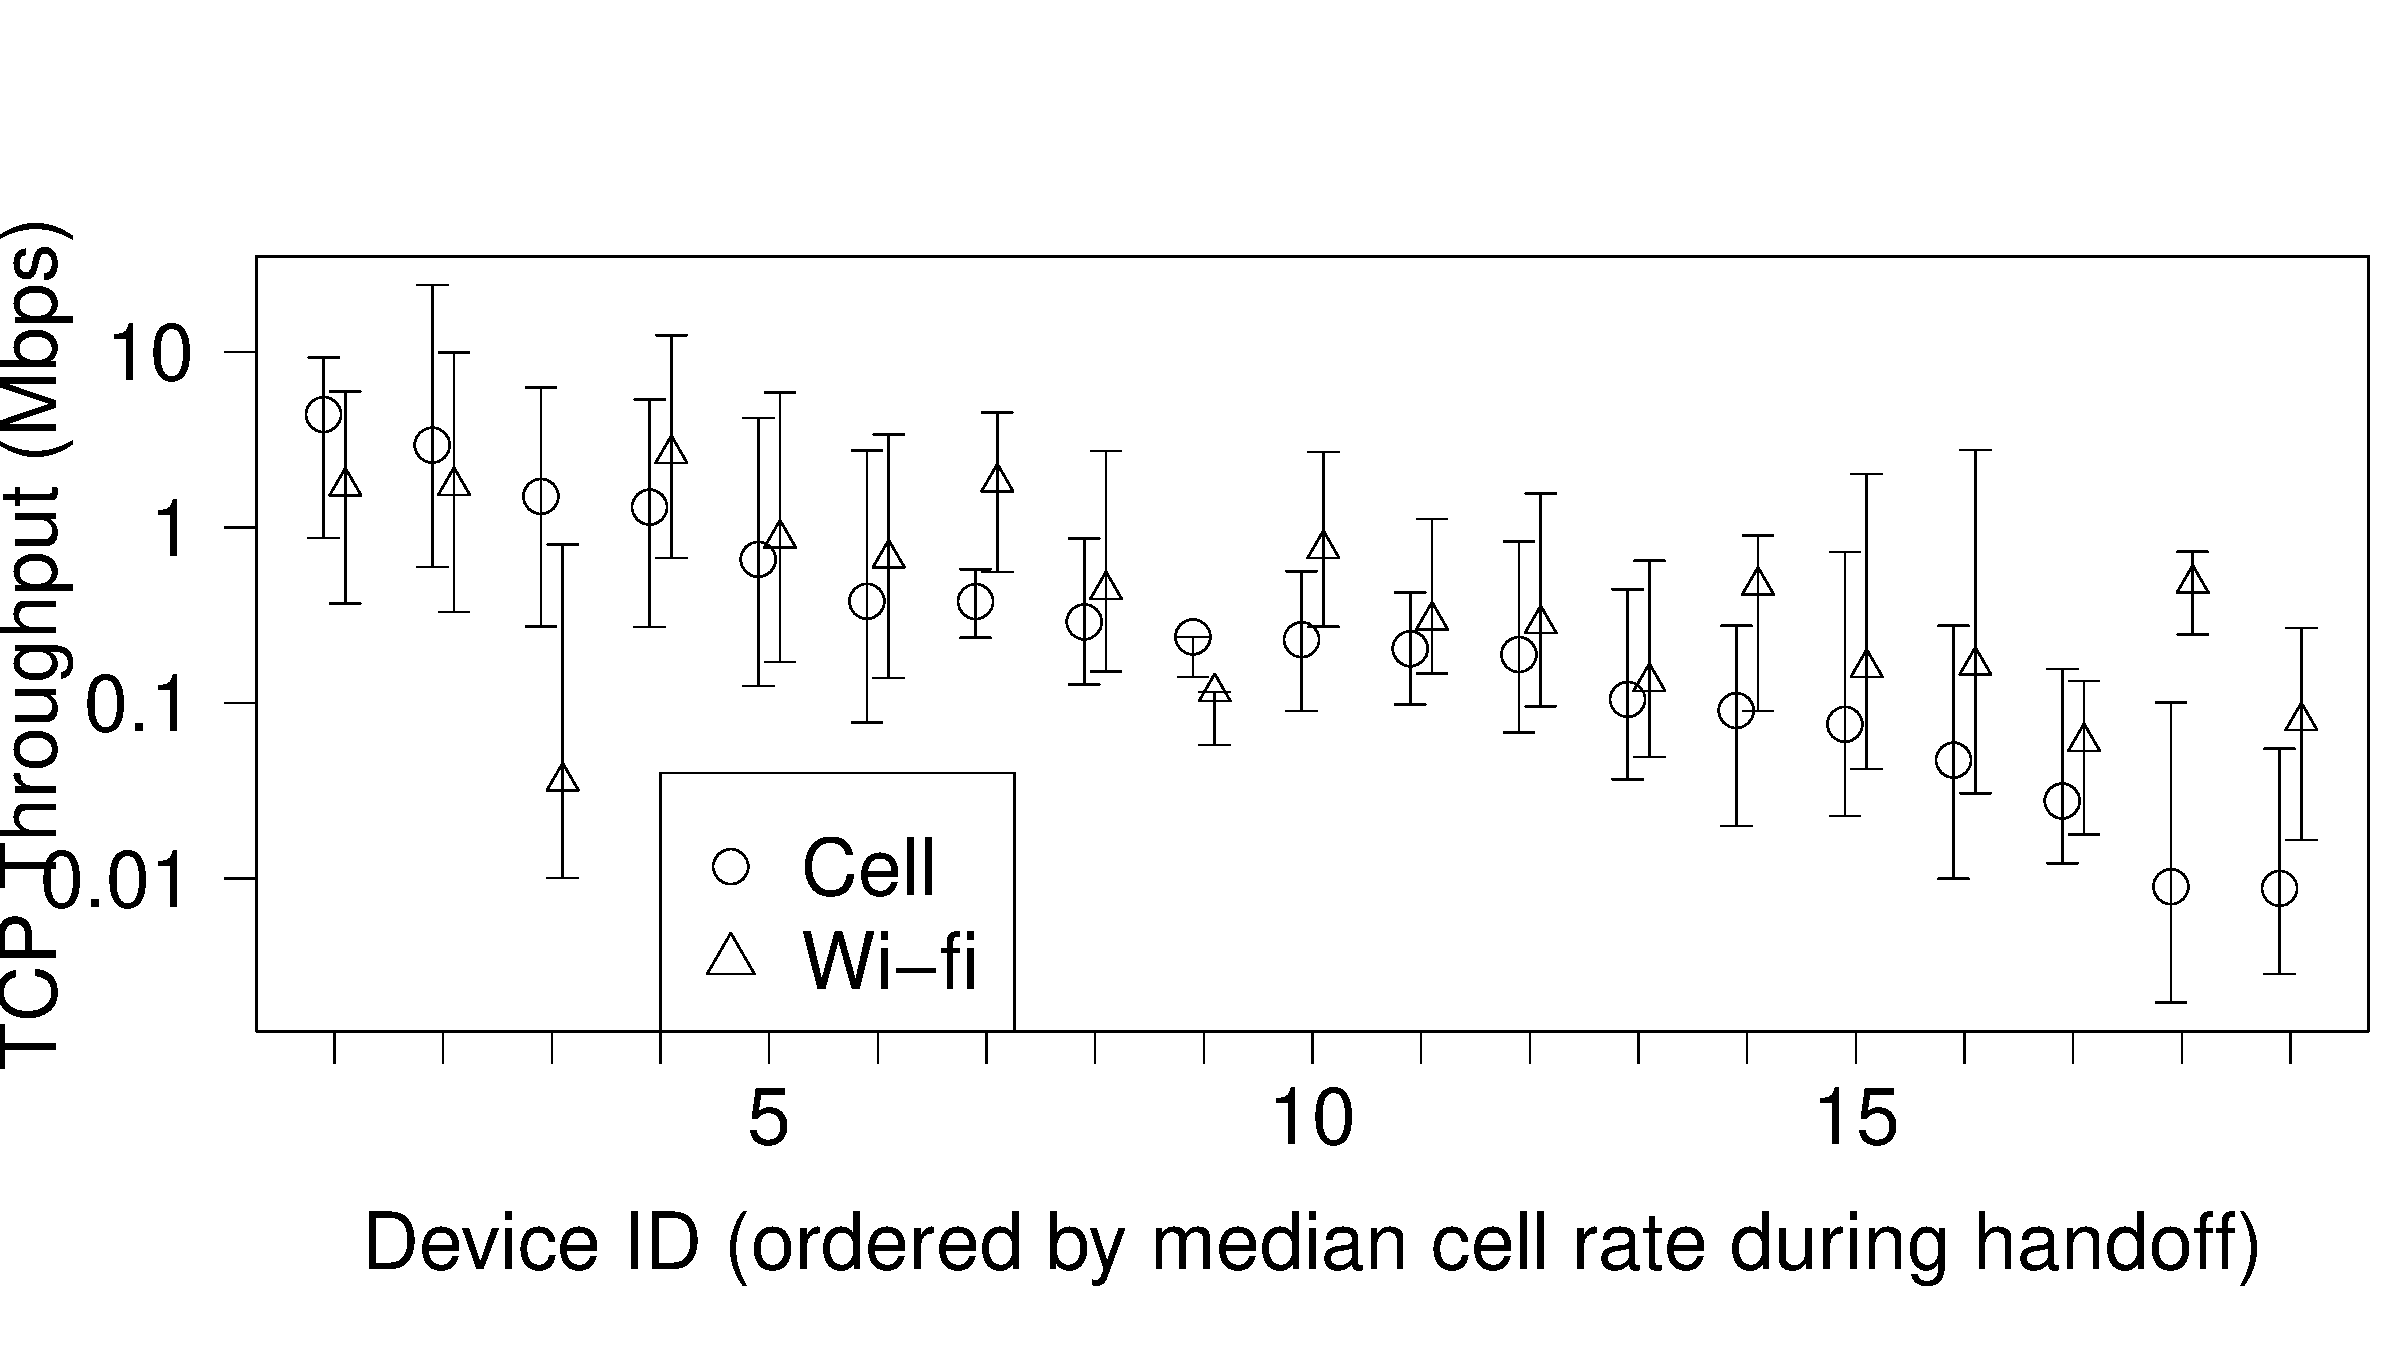
\includegraphics[width=\columnwidth]{plots/handoff_rates.pdf}
\caption{TCP Throughput observed during the hour of the handoff. \emph{The three users that have LTE connections observed a better TCP throughput over LTE in comparison to \wifi in the hour of the handoff. Error bars indicate the 91st and 9th percentile}.}
\label{fig:compare-handoff}
\end{figure}




\tbd{We performed a traceroute from our server to the egress link and found }





\section{Controlling Mobile Traffic}
In this section, we use two case studies to highlight some of the 
advantages \meddle provides as a new point of control 
for mobile networking traffic. We then discuss several new applications 
we are currently building.

\subsection{Packet Filtering}
Packet filtering is a common technique implemented in 
today's middleboxes. These can be used for implementing 
security policies, censoring content or preventing applications 
from harming the network (\eg, P2P). In \meddle, we use 
packet filtering to enable a number of features that are 
currently either unavailable or poorly implemented.

\noindent\textbf{Device-wide ad blocking.} Content and service providers 
typically use revenue from advertisements to cover their costs, enabling 
``free'' access for users. Given the additional costs in terms of data volume, 
battery consumption and potentially reduced privacy from tracking, it is unclear 
just how ``free'' these services truly are. Vallina-Rodriguez~\etal~\cite{Vallina-rodriguez:2012:AdCache} observe
that ads account for 5\% of daily traffic from more than 50\% of
Android users in a large European ISP. 

There is no current standard for opting 
out of unsolicited advertising; those that exist for tracking are not widely supported. 
Not surprisingly, many users have turned to software that blocks ad and analytic servers. 
For example, more than 20\,million users have installed 
AdBlockPlus~\footnote{http://www.adblockplus.org}, one of several tools for this purpose. 
Unlike the desktop environment, mobile device browsers do not provide support for 
ad blocking; further, most interactions occur inside of apps where browser plugins 
cannot help. 

\meddle makes it easy to implement an efficient, device-wide ad blocker. 
In our current implementation, we use a DNS-based filter to
block ads, analytics, and mediation sites.\footnote{The service is disabled by default, so users must 
opt in to enable blocking.} A key feature of our solutions is that it works 
regardless of whether SSL is used because DNS requests occur out of band 
from the secure connection. Further, the response from the DNS request is {\tt localhost}, 
meaning that devices will generate no external network traffic when failing 
to resolve the ad servers. 

\tbd{Describe figure.}

\begin{figure}
\centering
        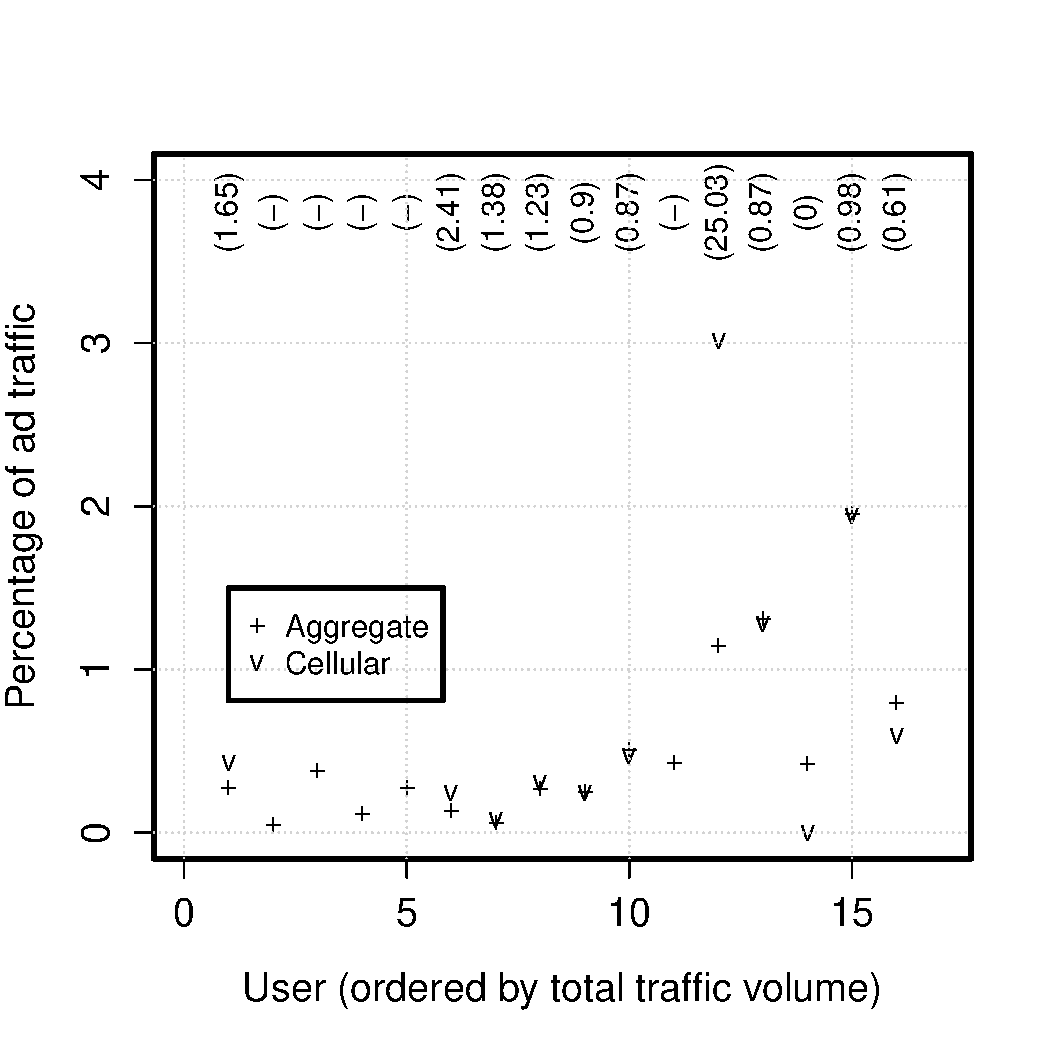
\includegraphics[width=\linewidth]{./plots/userAdsShare}
  \caption{\tbd{caption}}
  \label{fig:adblocking}
\end{figure}


Our ad blocking engine relies on a publicly available list of domains for ads and
analytics~\cite{YoyoAds}; we augment this list of domains using 
recent research on mobile ads~\cite{hornyack:appfence,
  Leontiadis:2012:AdsMobile}. From our initial deployment, we observed a 0.05\% to 0.8\% reduction
in total traffic at each mobile device due to our ad blocking engine. 
\tbd{Ashwin: is this still true?}
In addition to the DNS-based filter, we are currently implementing a filter that blocks 
requests for URLs matching a regular expression, as done by AdBlockPlus.

\tbd{Mention Privad gateway}

\noindent\textbf{Do not disturb.} 
Many users do not turn off their devices at night, even while asleep. In our study, we found that 
\tbd{XX}\% of devices were active for at least one entire 24-hour period. Network 
traffic occurring during those periods is generally not helpful for the user; worse, 
such traffic may cause audible alerts that wake up the user. In part to address this, 
iOS 6 introduced a ``Do not disturb'' feature that silences the phone and \emph{reduces} 
network activity. We are unaware of such support on Android.

\meddle enables a cross-platform and cross-device ``Do not disturb'' for network 
traffic. Users specify the hours when traffic should be blocked and the corresponding 
meddlebox will drop all traffic. Further, users can specify hosts that should \emph{not} be 
blocked. 

\noindent\textbf{Parental controls.} 
Existing parental controls for mobile devices tend to focus on which apps a user 
cannot run. For example, a parent can block the Facebook app on an iOS device. 
To the best of our knowledge, there is no way to prevent a user from using a 
Web browser to access the Facebook site, unless all Web browser activity is blocked. 

In general, this would be too prohibitive. Using \meddle, we can blacklist traffic for 
all IPs known to belong to a content or service provider. For example, to block 
Facebook we would block IPs belonging to Facebook, as well as any traffic using Facebook 
SSL certificates (\eg, for accessing content hosted by CDNs). 

\subsection{Traffic Manipulation}
An advantage of \meddle is that it provides isolation from carriers' in-network 
middleboxes, which may block, modify or shape certain network traffic. However, 
toward the goal of improving transparency in mobile networks (especially for 
non-\meddle users), we would like to be able to identify when, how and what 
network traffic is subject to carrier manipulation. 

In this section, we describe how we use \meddle to detect HTTP interference via 
in-flight Web page changes. We believe our technique 
is general to other protocols. 

The problem of HTTP interference was highlighted 
by Reis et al.~\cite{reis:tripwires}. The authors demonstrated that although a small 
precent of users were affected by in-flight changes, those changes tended to introduce 
vulnerabilities such as overflows and cross-site scripting (XSS) attacks. They proposed and deployed 
\emph{Web Tripwires}, Javascript code that detects in-flight page changes. The main 
limitation of this study is that the approach works only for sites that include a tripwire on their 
own pages.

\noindent\textbf{Web Tripnets.} Using \meddle, we extended tripwires to alleviate this 
limitation. Namely, we use \meddle to inject a tripwire on \emph{any} page without requiring 
support from Web site developers -- an approach we call a \emph{Web Tripnet}.

When enabled, the Web tripnet works as follows (depicted in Fig.~\ref{fig:tripnet}). First, the device requests a Web page via 
HTTP (1). Because the \meddle connection is encrypted, the device's 
provider cannot alter the page in flight. When the Web server response arrives at 
the \meddle server (2), we insert a Web tripwire before forwarding the response to the user. 

To detect whether the carrier would have manipulated the 
page without \meddle, we create a \emph{pigeonhole} by configuring the device's VPN settings to send 
traffic for a particular site in the clear. When the Web tripwire attempts to load another copy 
of the Web page (3), the request is redirected (using DNS) to a transparent proxy that forwards the request to the intended server, 
retrieves the Web page and delivers it to the device in the clear (thus exposing it to carrier manipulation). 
Upon receiving the page over an unencrypted channel, the device's browser sends both 
versions of the Web page (tunneled and untunneled) to the \meddle server for analysis. 

\begin{figure}
\centering
        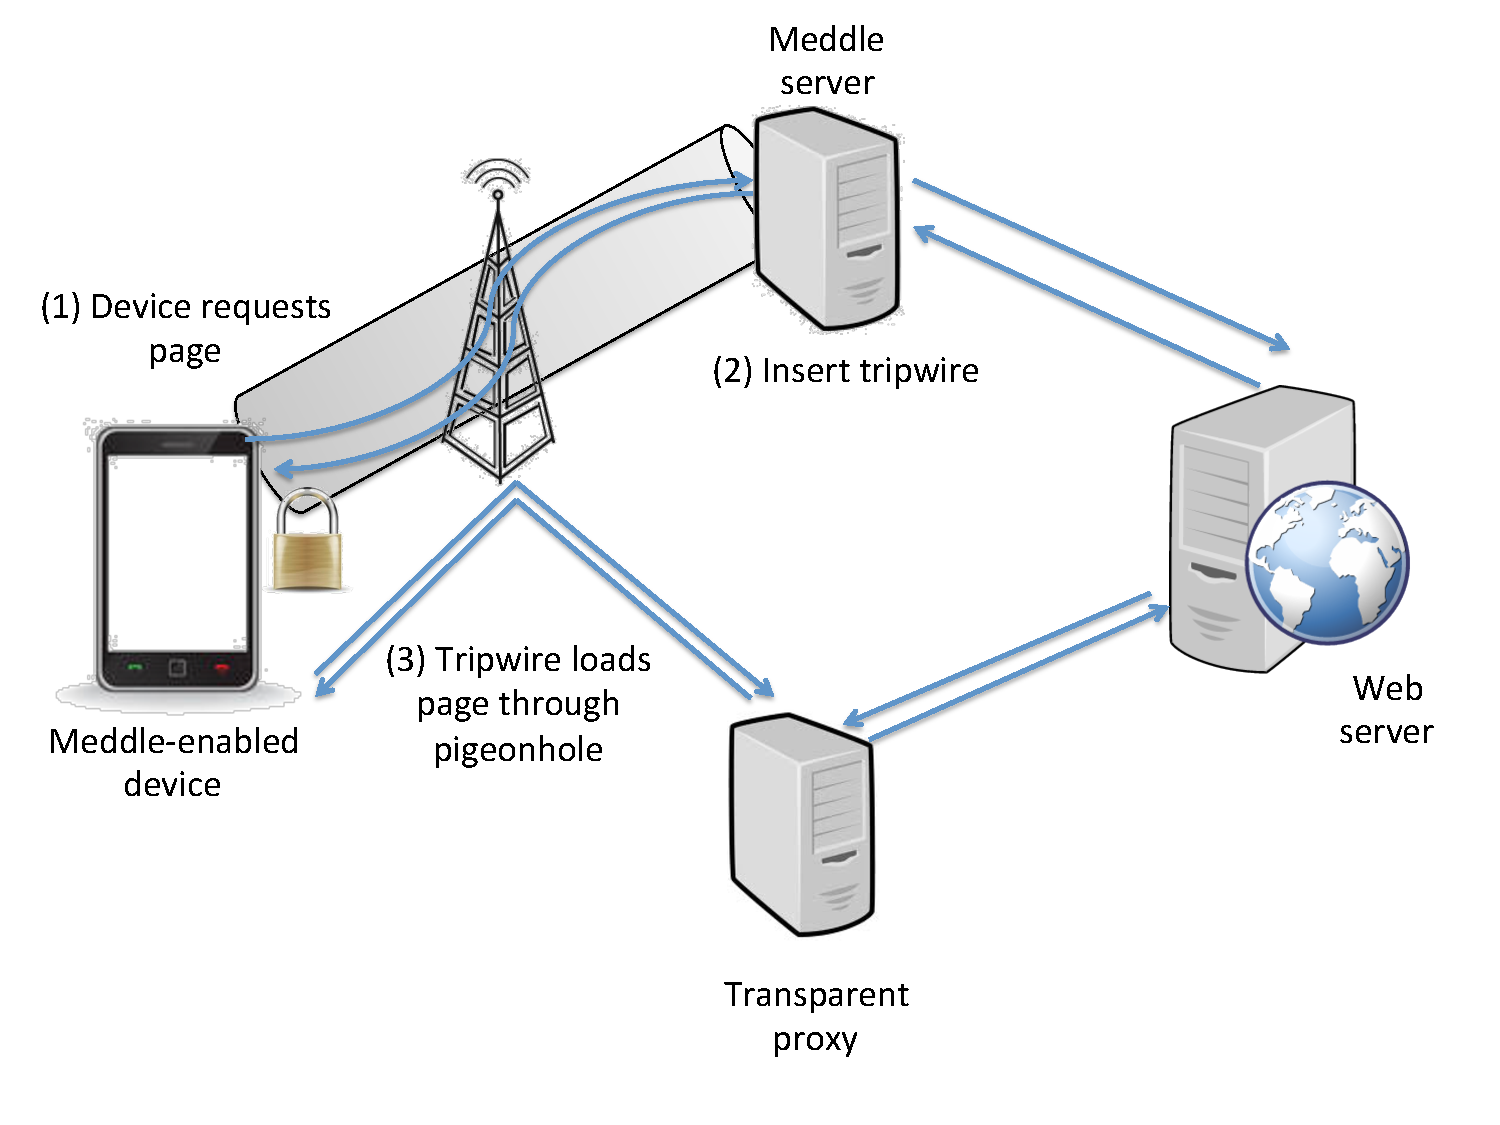
\includegraphics[width=\linewidth]{figs/tripnet.pdf}
\vspace{\figcapspace}
  \caption{Overview of the \meddle Web tripnet. A Web page is loaded 
through the VPN tunnel, where a meddlebox inserts a Web tripwire. The 
tripwire causes the browser to reload the Web page using the address of a
transparent proxy server that is accessed using an unencrypted connection. 
After the proxied version of the page is loaded, a message is sent to the user if 
the pages differ due to ISP interference. }
  \label{fig:tripnet}
\vspace{\postfigspace}
\end{figure}

\noindent\textbf{Experimental Results.} We conducted a survey of ISP HTTP injection using two US carriers (Verizon and T-Mobile) 
and one French carrier (XXX). To determine if the user agent can impact manipulation from 
carriers, we tested using Android, iOS and a desktop (tethered) browser. We tested the top 
100 sites according to Alexa, in addition to a random sample of 100 of the 10,000 most popular 
sites. Our analysis did not identify any carrier manipulation. This is not entirely surprising, 
since most manipulation identified by Reis et al. occurred due to software installed inside 
a user's network.

An interesting observation is that 
we found one example where Facebook over Verizon included a promotional link specific to 
Verizon, even when the connection was proxies through a host at the University of Washington. 
Further analysis showed that the Squid proxy's {\tt X-Forwarded-For} field was being populated 
with an address in Verizon's network, and Facebook was modifying the page accordingly. When 
we removed the {\tt X-Forwarded-For} field, the promotional link no longer appeared. 

\subsection{New Applications}

\meddle allows researchers to explore the space of applications that offload 
networking traffic from mobile devices to server where power and data quota 
are less scarce. We envision several important applications that can benefit 
from our approach.

\begin{itemize}
\item \textbf{P2P offloading.} P2P services tend to benefit from multiple connections 
and symmetric bandwidth contributions from participating hosts. Both of these are 
costly in the mobile environment. \meddle can ease these costs by offloading the 
logic for maintaining P2P connections to a meddlebox.
\item \textbf{Privad.}  Instead of simply blocking ads, \meddle is an ideal location 
to deploy anonymizing systems that support targeted advertising, as suggested by 
Guha et al.~\cite{guha:privad}. 
\item \textbf{Tor.} \meddle improves privacy in mobile networking by encrypting the 
connection from the mobile device to the \meddle server. We can further improve 
privacy and anonymity by providing a Tor meddlebox that establishes and manages 
onion-routed connections.

\end{itemize}


%Example Apps (highlight things we can do with meddle)
% - Begin with a sentence/intro-para on using middleboxes to offloading activities and offer device wide services
% - Middlebox based packet monitoring 
%      - cross * possible
%      - passive - real traffic 24x7 
%      - actual users
%      - Network traffic characterization
%         - Longitudinal study of network traffic
%         - understand behavior of apps
% - Device wide services - service like packet filtering that is not limited to an app 
%     - Ad blocking
%     - Platform for malware detection and blocking
%     - Parental controls 
% - Deployment of new protocols and services 
%   - Users can opt in for specific service
%   - Mobile story for services like FreeDOM, CCNs, etc.
%   - service in a VM where users opt in for services
% - Generic Proxy
%   - Privad
%   - Anti-censorship

\section{Discussion}
\label{sec:discussion}
In this section, we discuss several key issues and limitations for an indirection-based 
deployment such as \meddle.
 
\noindent\textbf{Privacy and trust.} As discussed in Section~\ref{subsec:currdeploy}, we 
collect traces from users as part of an IRB-approved study. We take great care in 
protecting user privacy -- data is encrypted before being stored, the private key is 
not stored on the server where data is recorded and any PII accidentally sent in the 
clear is stripped from our datasets as soon as we identify it. 

While this fine-grained data is useful for informing the design of meddlebox solutions (\eg, 
identifying and stripping personally identifiable information from unencrypted 
HTTP traffic), it can be prohibitive for a large-scale study. In the next phase of 
our deployment (currently under IRB review) we will capture only packet headers 
and lengths. With a lower privacy risk, we believe we can recruit a larger number 
of users and obtain informed consent via a Web site. 

Regardless, users may still be uncomfortable with sending all their traffic through a 
\meddle service, be it in a hosting center or in the cloud. We are making all of 
our code open source so that users can install \meddle on servers in their 
own networks (\eg, in their home network). Users may opt to use this option instead; however, they will also be responsible 
for updating \meddle to include the latest new features and bug fixes. We expect 
that most users interested in running \meddle will be content with using our hosted 
\meddle service with anonymized packet headers being collected. 

\noindent\textbf{Acceptable use.} Similar to any service providing Internet access, 
\meddle needs an acceptable use policy (AUP) to ensure that we are not liable for 
user activity. We model our AUP after the one provided by EC2, one of our potential 
hosting providers. Users are informed of this AUP at install time. If we are notified 
of an AUP violation, we can isolate the user generating the traffic because each 
user is given separate certificate-based credentials.

\noindent\textbf{ISP objections.} Many mobile carriers deploy in-network middleboxes 
for traffic engineering purposes. By tunneling \emph{all} traffic, these boxes lose the 
ability to implement ISPs' policies, which can lead to suboptimal performance for 
other users sharing the network. 

We believe such concerns are either overblown or misguided. First, we do not 
expect \emph{every} device to run \meddle. If we were to attract even 1\% of 
mobile users that would be a surprisingly huge success. Thus we do not expect 
\meddle to significantly impact overall traffic in a mobile network. Second, if \meddle 
traffic were to become a significant traffic engineering challenge, we argue that 
such information, and the policies that address this challenge, need to be 
transparent to users. The current model of transparent middleboxes is not 
in the spirit of an open Internet.

\noindent\textbf{Scalability and reliability.} If successful, \meddle will 
face scalability and reliability problems as the number of users increases. 
We believe that, in return for valuable measurement and experimentation data, 
we can justify funding to support some number of thousands of users. For a 
larger deployment, we may have to consider a paid service or alternative 
economic models. By running the service in the cloud and using DNS-based 
redirection, we expect service unavailability to be relatively rare. Importantly, 
we expect that mobile connectivity in general will be less reliable than connections 
to \meddle servers.

\noindent\textbf{Limitations.} We believe that \meddle enables a large number 
of interesting studies and experiments in the mobile environment. However, we 
do not claim it is a panacea. 

First, \meddle captures only network traffic. It does 
not allow us to gain access to sensors on the device, information about what 
apps are running or control over those apps on the device. An interesting question 
is what are the limits of what one can infer from a device's network traffic alone. 
We have shown that iOS network traffic exhibits clear, identifiable differences 
when plugged in versus running on battery, lending evidence that we can successfully 
infer properties of the phone previously available only by querying from an app 
on the device. Likewise, we used SSL certificates to distinguish which app generates 
requests to a CDN.

Second, \meddle may miss some data traffic. For example, we identified that 
iOS push was using signaling on a circuit-switched channel (SMS). We believe 
the volume of ``missing'' traffic is small; however, it remains to be seen how 
this holds generally and over time. As mobile networks transition to all-IP, it will 
be interesting to see if an approach like \meddle can capture all of a device's traffic.

Last, \meddle incurs costs that may dissuade adoption. We discussed several of the 
overheads based on establishing a VPN tunnel. One area of future work is to improve 
VPN protocols to reduce the time to establish a connection. 


\section{Related Work}
\label{sec:related}

The network behavior of mobile systems has implications for battery life, 
data-plan consumption, privacy, security and performance, among others. 
When attempting to characterize this behavior, researchers face a number 
of trade-offs: compromising network coverage (limiting the number and type of ISPs measured), 
portability (limiting the device OSes) and/or deployability (limiting subscriber coverage).
\platname compromises 
none of these, enabling comprehensive measurements across carriers, devices and access 
technologies. Table~\ref{tab:relatedCompare} puts our approach in context with previous 
approaches for measuring the network behavior of mobile systems. 

\begin{table*}[t]
\begin{center}
{\footnotesize
\begin{tabular}{|l|l|l|l|l|}
\hline
 & \textbf{Network Coverage} &  \textbf{Portability} &  \textbf{Deployment model} &   \textbf{Meas. Type}  \\ \hline
AT\&T/Telefonica study~\cite{vallina-rod:ads,gerber:passivespeed} & Single carrier & All OSes & Instrument cell infrastructure & Passive \\ \hline
WiFi study~\cite{chen:wifi} & Single WiFi network & All OSes & Instrument WiFi network & Passive \\ \hline
PhoneLab/TaintDroid~\cite{enck:taintdroid} & Multiple networks & Android & Install custom OS & Active/Passive \\ \hline
MobiPerf~\cite{wang:middleboxes}/SpeedTest~\cite{sommers:cellwifi} & Multiple networks & Android & Install App & Active \\ \hline
\platname & Any network & Android / iOS & VPN configuration & Passive \\ \hline
\end{tabular} }
\end{center}
\label{tab:relatedCompare}
\caption{Comparison of alternative measurement approaches. \platname is the first approach to cover all access networks and most device OSes, capturing 
network traffic passively and with low overhead via VPN proxying.}
\end{table*}%

Traces from mobile devices can inform a number of interesting analyses. Previous work 
uses custom OSes to investigate how devices waste energy~\cite{pathak:eprof}, network bandwidth and 
leak private information~\cite{enck:taintdroid,hornyack:appfence}. Similarly, AppInsight~\cite{ravindranath:appinsight} and PiOS~\cite{egele:pios} can inform 
app performance through binary instrumentation and/or static analysis. In this work, we explore the opportunity to use network traces 
alone to reveal these cases without requiring any OS or app modifications.

Network traces from inside carrier networks provide a detailed view for large numbers 
of subscribes. For example, Vallina-Rodriguez~\etal~\cite{vallina-rod:ads} uses this approach to characterize performance and 
the impact of advertising. Gerber \etal~\cite{gerber:passivespeed} similarly use this approach to 
estimate network performance for mobile devices.  \cite{maier:mobtraffic} \cite{chen:wifi}
Similar to these approaches, \platname provides continuous passive monitoring of mobile network 
traffic; however, \platname is the first to do so across all networks to which a device connects.

Last, active measurements~\cite{wang:middleboxes,sommers:cellwifi} allow researchers to understand network topologies and instantaneous 
performance at the cost of additional, synthetic traffic for probing. In contrast, \platname uses 
passive measurements to characterize the traffic that devices
naturally generate.

%%% Local Variables: 
%%% mode: latex
%%% TeX-master: "main.tex"
%%% End: 


\section{Conclusion}
\label{sec:conclusion}

This paper described how we use proxying to provide a comprehensive view of Internet traffic 
generated by mobile devices. The key observation is that most devices already support traffic 
indirection via VPNs; by using VPN servers as proxying and instrumenting them to record 
traffic flows, we passively monitor traffic from mobile devices regardless of access 
technology, device or OS. Using this unique view of mobile-device traffic, we conduct 
controlled experiments and user studies to characterize and classify apps and to identify 
PII leakage. As part of future work, we are investigating additional 
techniques to improve traffic classification and to identify PII. To understand network 
behavior from a much more diverse set of users and devices, we are deploying 
a second study that is IRB-approved for a larger set of users without requiring 
in-person interviews. 
\footnotesize
\bibliographystyle{abbrv}
\bibliography{biblio}

%\section{Push notifications and power management on iOS}
\label{sec:pushnotification}
\tbd{AL: this section is not intended to be as is in the final report,
but just a collection of results that can be incorporated in the final
document if needed.}

All the following experiments are performed on an iphone 4 with iOS
6.0.1.  At the beginning of each experiment we close all applications
and restart the iphone. The iphone is connected in wifi to a
controlled access point on which we perform a tcpdump on the wifi
interface and monitor the wifi association between the access point
and the iphone. Each experiment lasts for around 1 hour. 

In a first set of experiments, we consider a default iphone setting with
3G and wifi enabled, and the iphone unplugged. This corresponds to a
typical setting for a user on move. 




\begin{figure}
\centering
        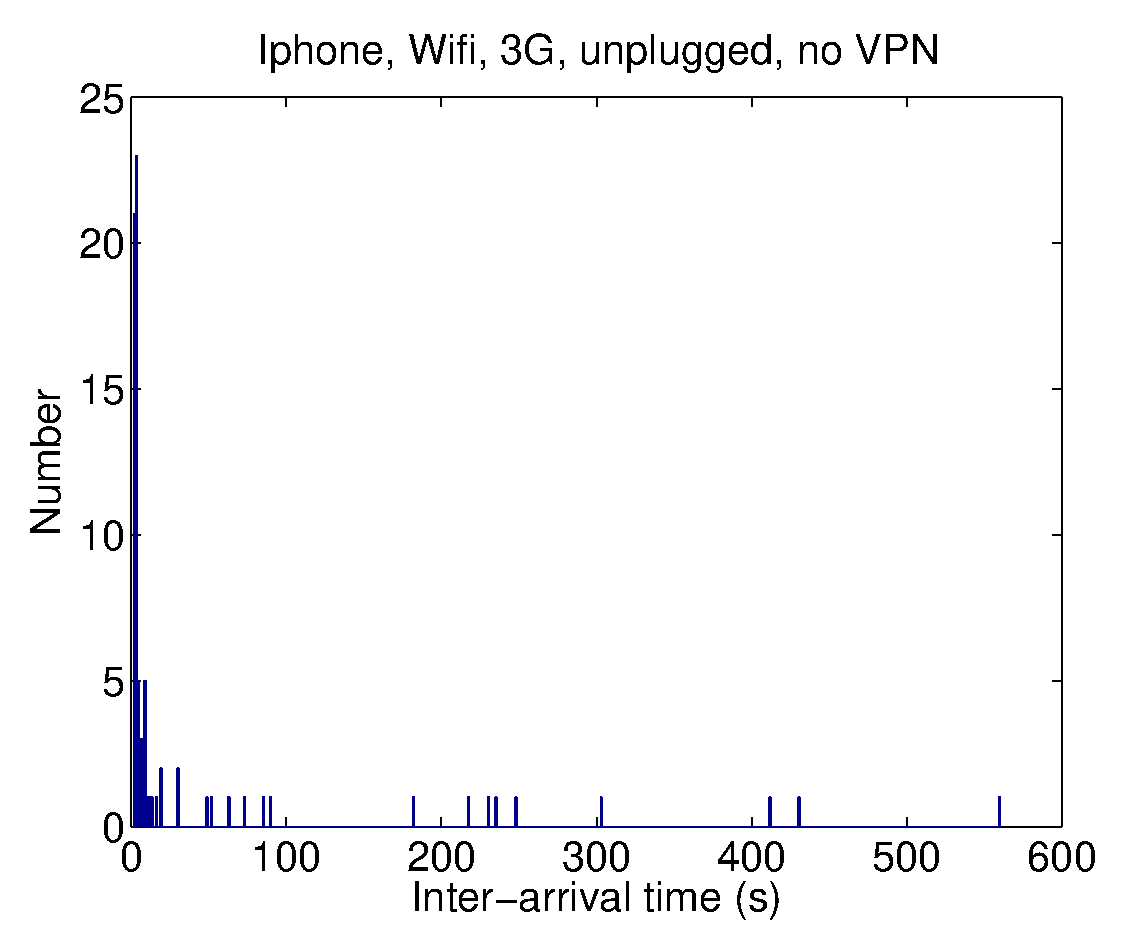
\includegraphics[width=0.8\linewidth]{../../code/pushNotification/Fig/bw_iphone_wifi_3g_unplug_novpn_interTs.eps}
  \caption{.}
  \label{fig:}
\end{figure}

\begin{figure}
\centering
        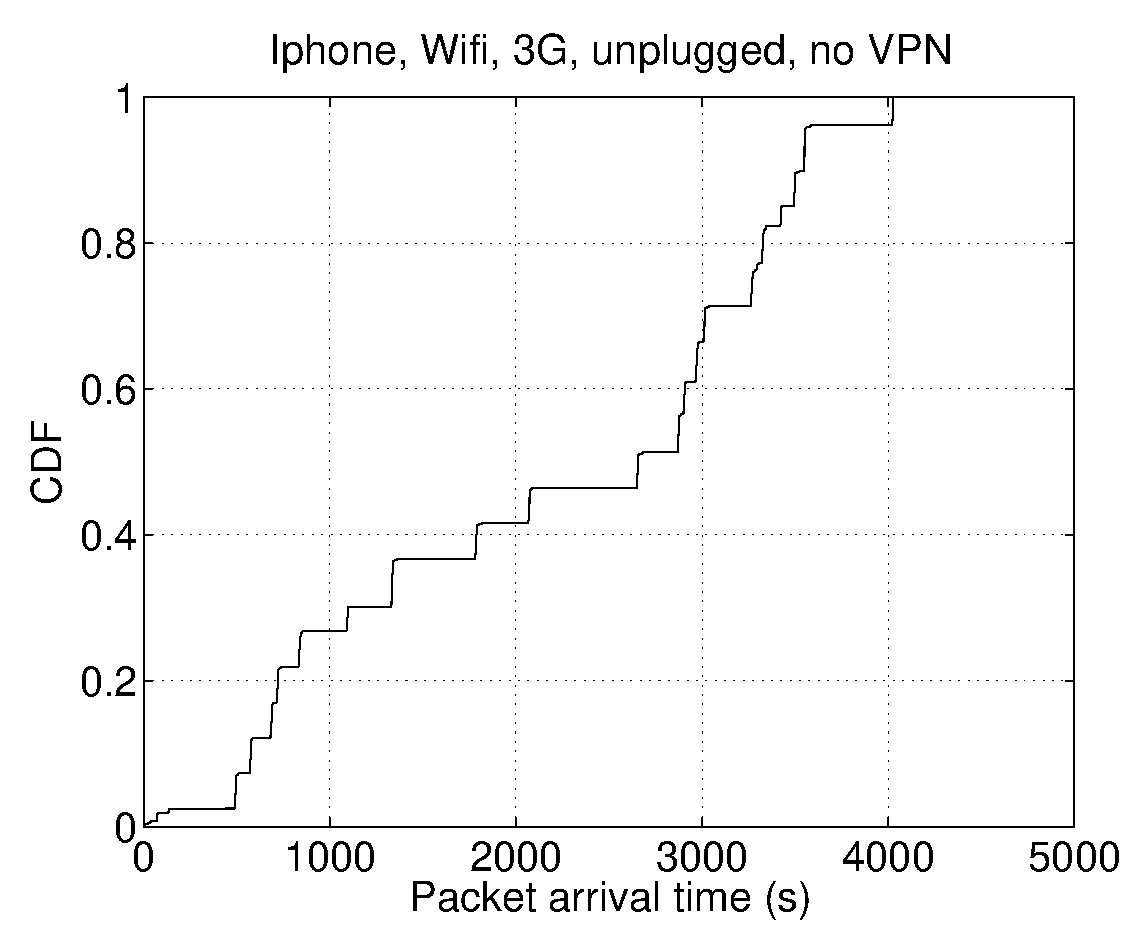
\includegraphics[width=0.8\linewidth]{../../code/pushNotification/Fig/bw_iphone_wifi_3g_unplug_novpn_ts.eps}
  \caption{.}
  \label{fig:}
\end{figure}

\begin{figure}
\centering
        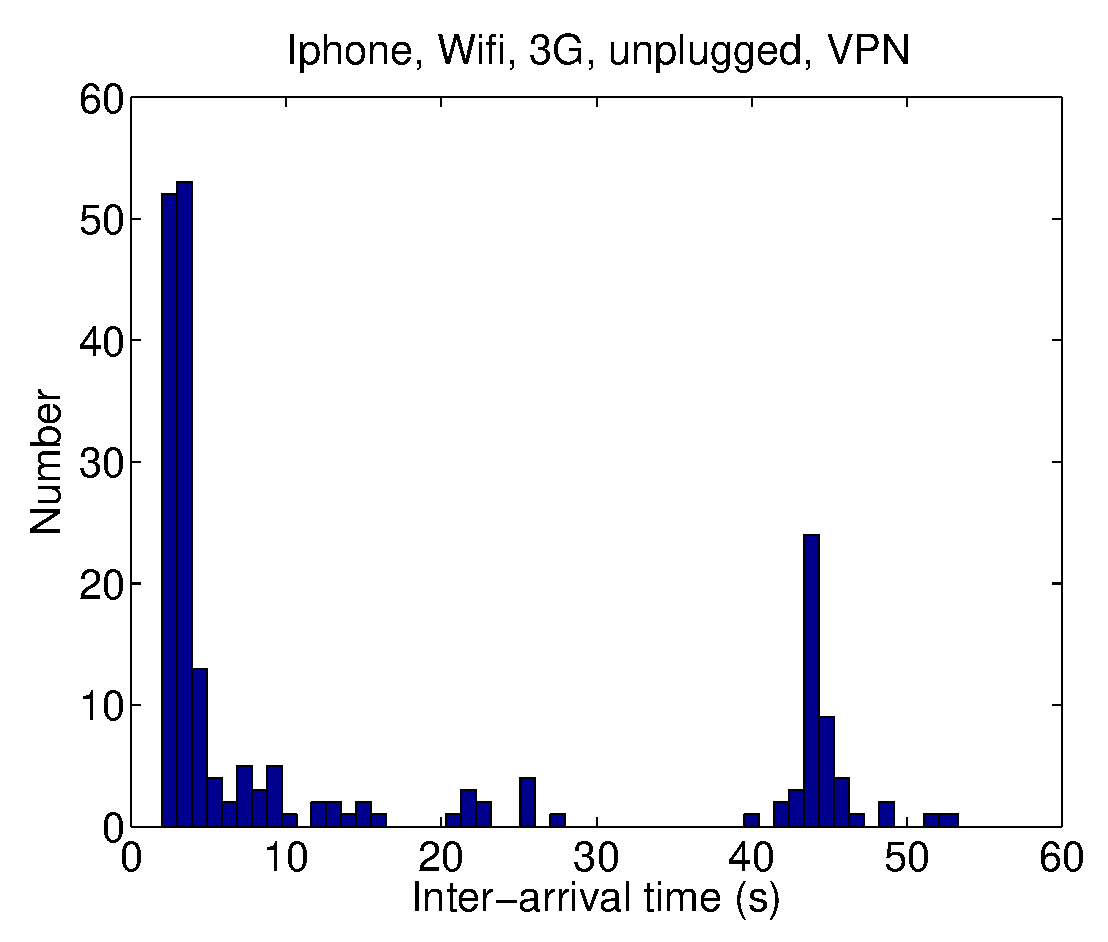
\includegraphics[width=0.8\linewidth]{../../code/pushNotification/Fig/bw_iphone_wifi_3g_unplug_vpn_interTs.eps}
  \caption{.}
  \label{fig:}
\end{figure}

\begin{figure}
\centering
        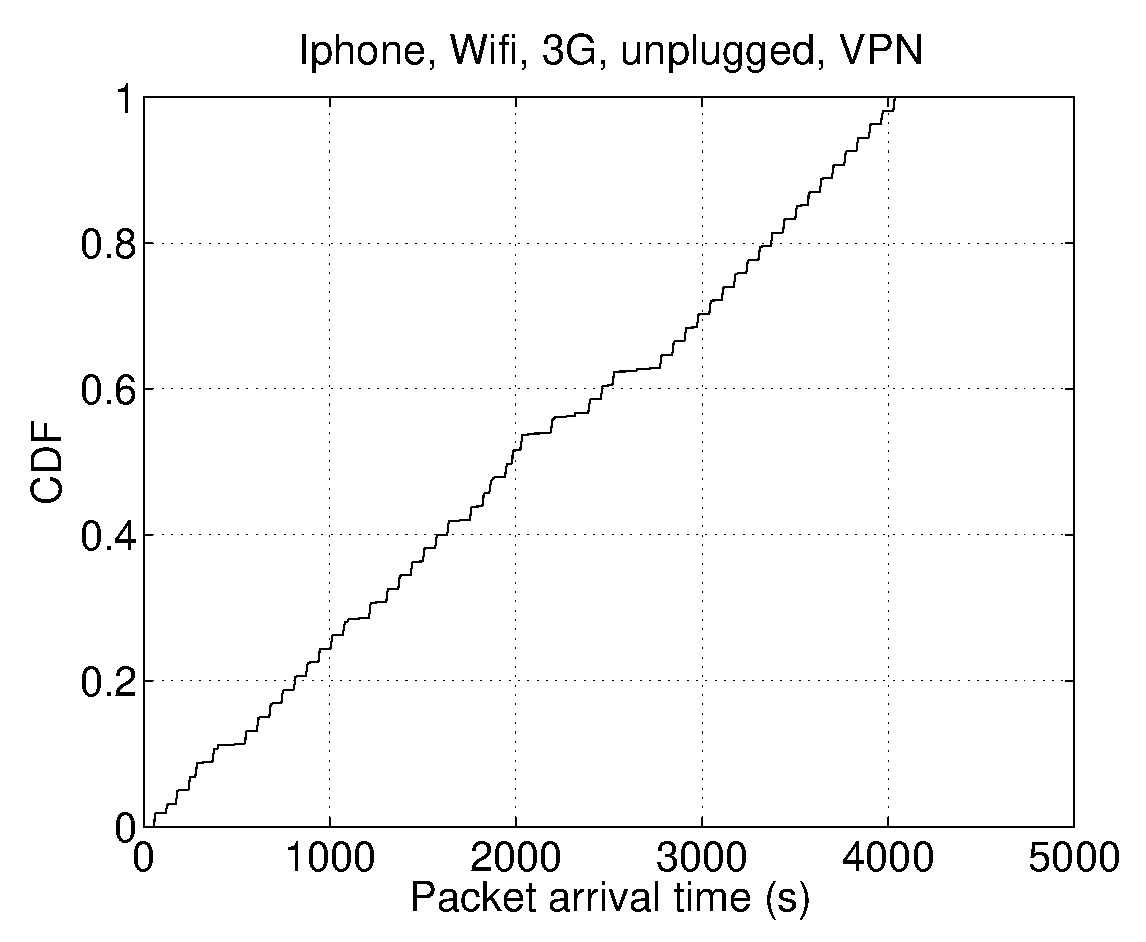
\includegraphics[width=0.8\linewidth]{../../code/pushNotification/Fig/bw_iphone_wifi_3g_unplug_vpn_ts.eps}
  \caption{.}
  \label{fig:}
\end{figure}

\begin{figure}
\centering
        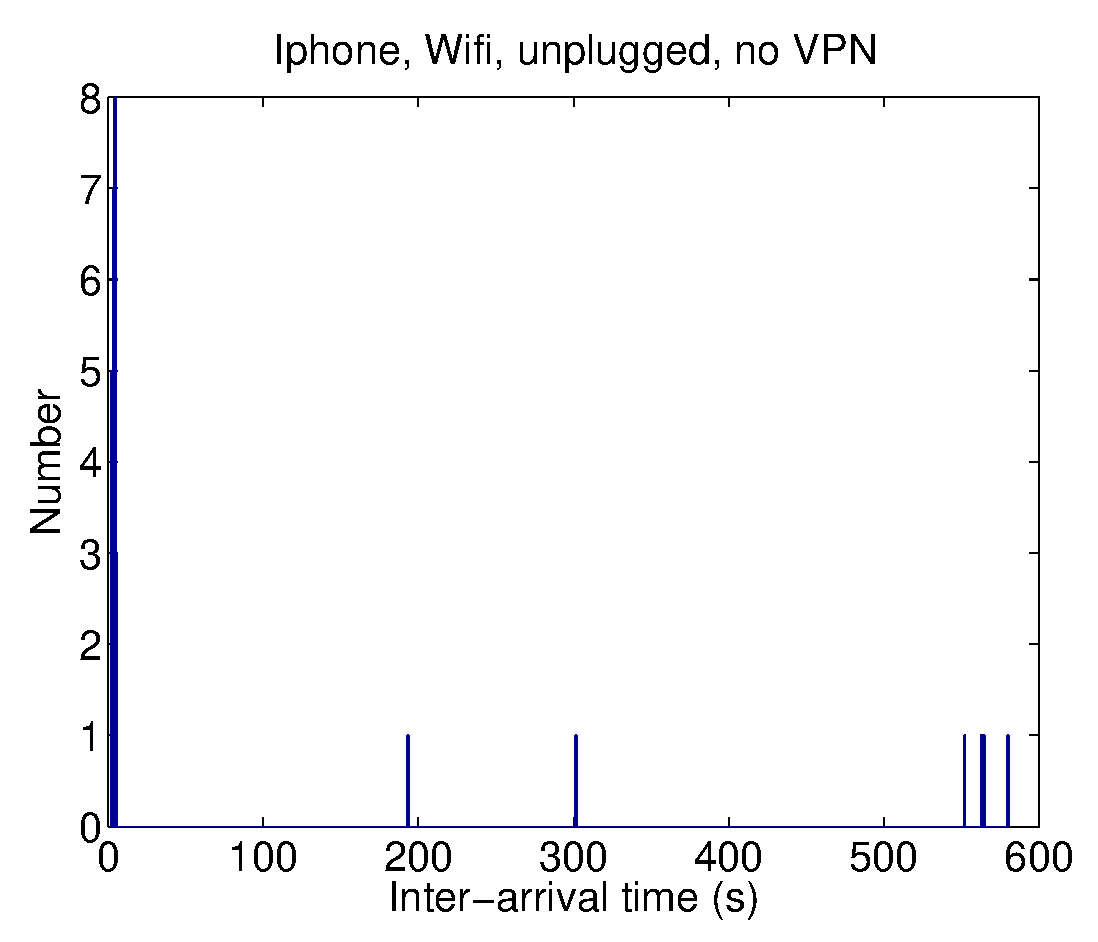
\includegraphics[width=0.8\linewidth]{../../code/pushNotification/Fig/bw_iphone_wifi_unplug_novpn_interTs.eps}
  \caption{.}
  \label{fig:}
\end{figure}

\begin{figure}
\centering
        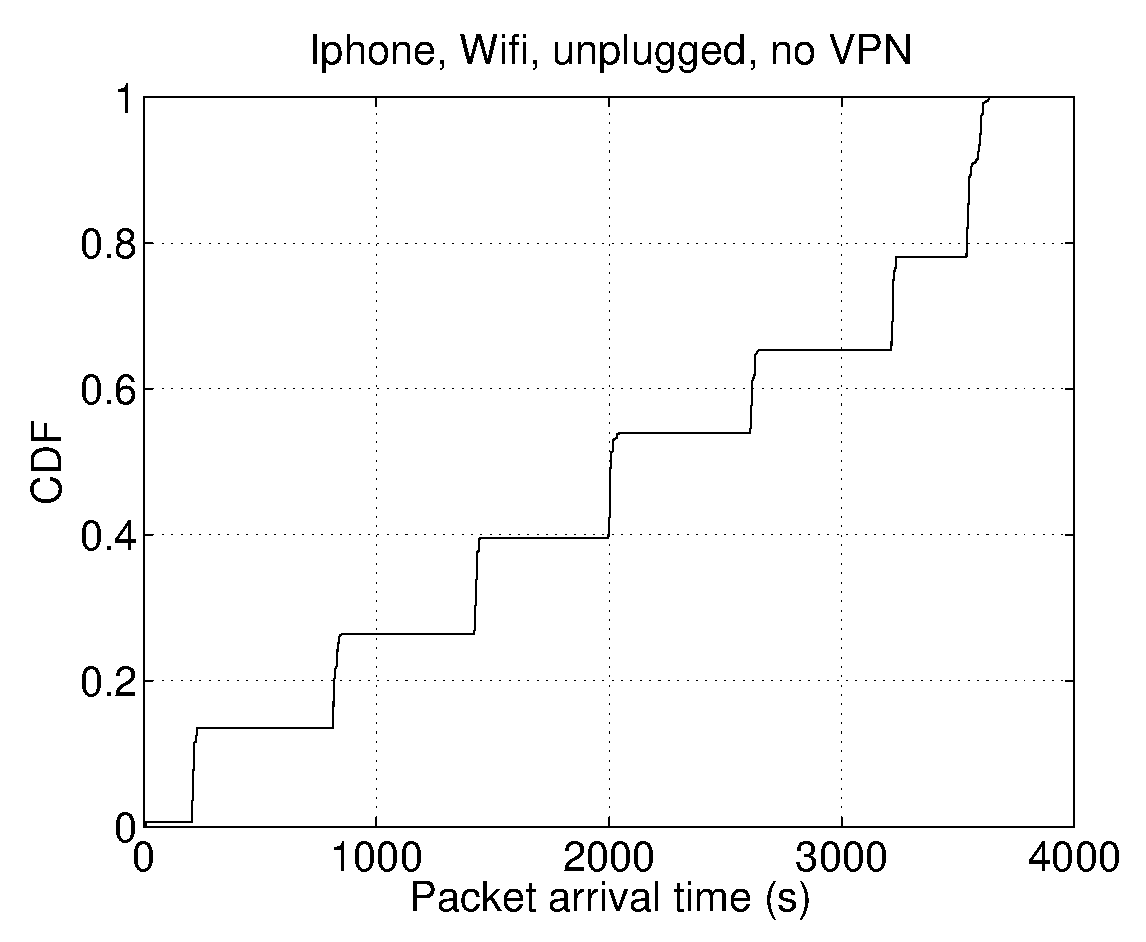
\includegraphics[width=0.8\linewidth]{../../code/pushNotification/Fig/bw_iphone_wifi_unplug_novpn_ts.eps}
  \caption{.}
  \label{fig:}
\end{figure}

\begin{figure}
\centering
        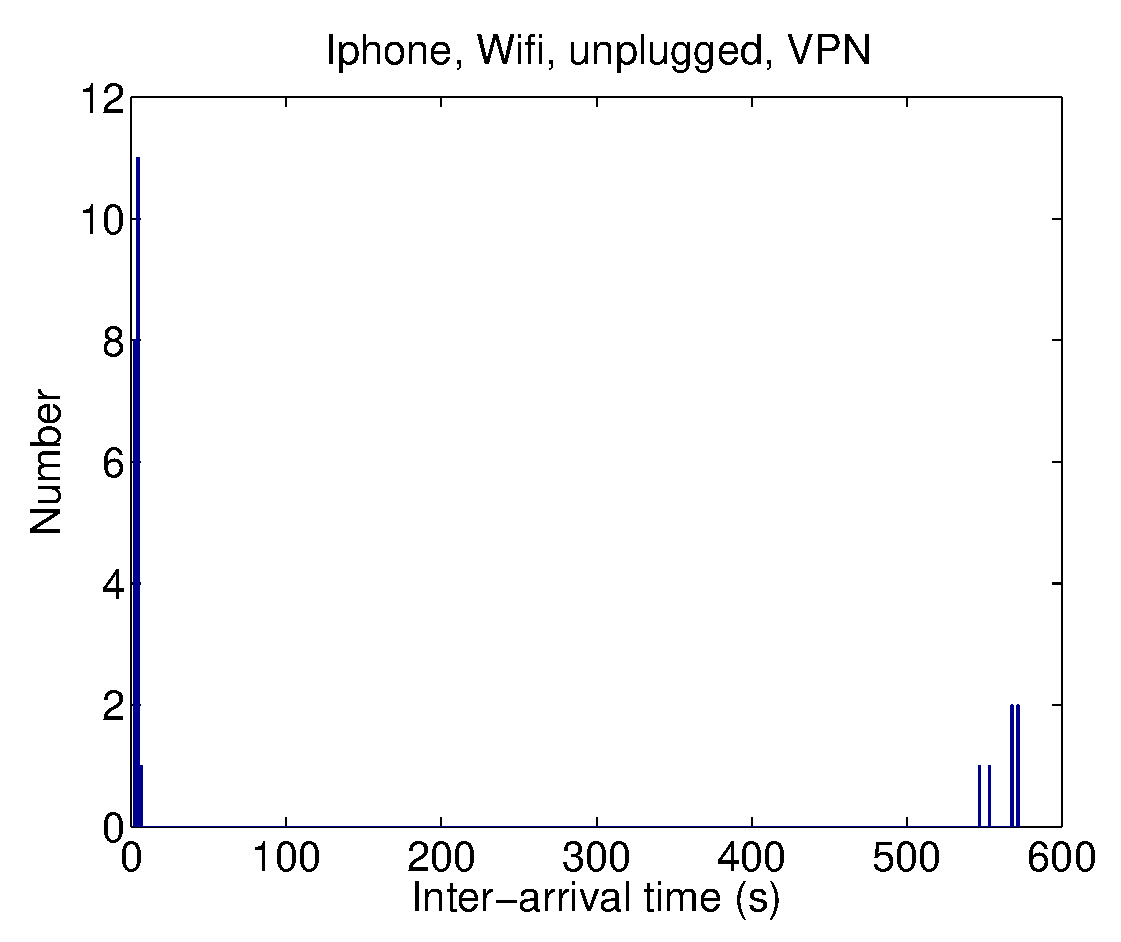
\includegraphics[width=0.8\linewidth]{../../code/pushNotification/Fig/bw_iphone_wifi_unplug_vpn_interTs.eps}
  \caption{.}
  \label{fig:}
\end{figure}

\begin{figure}
\centering
        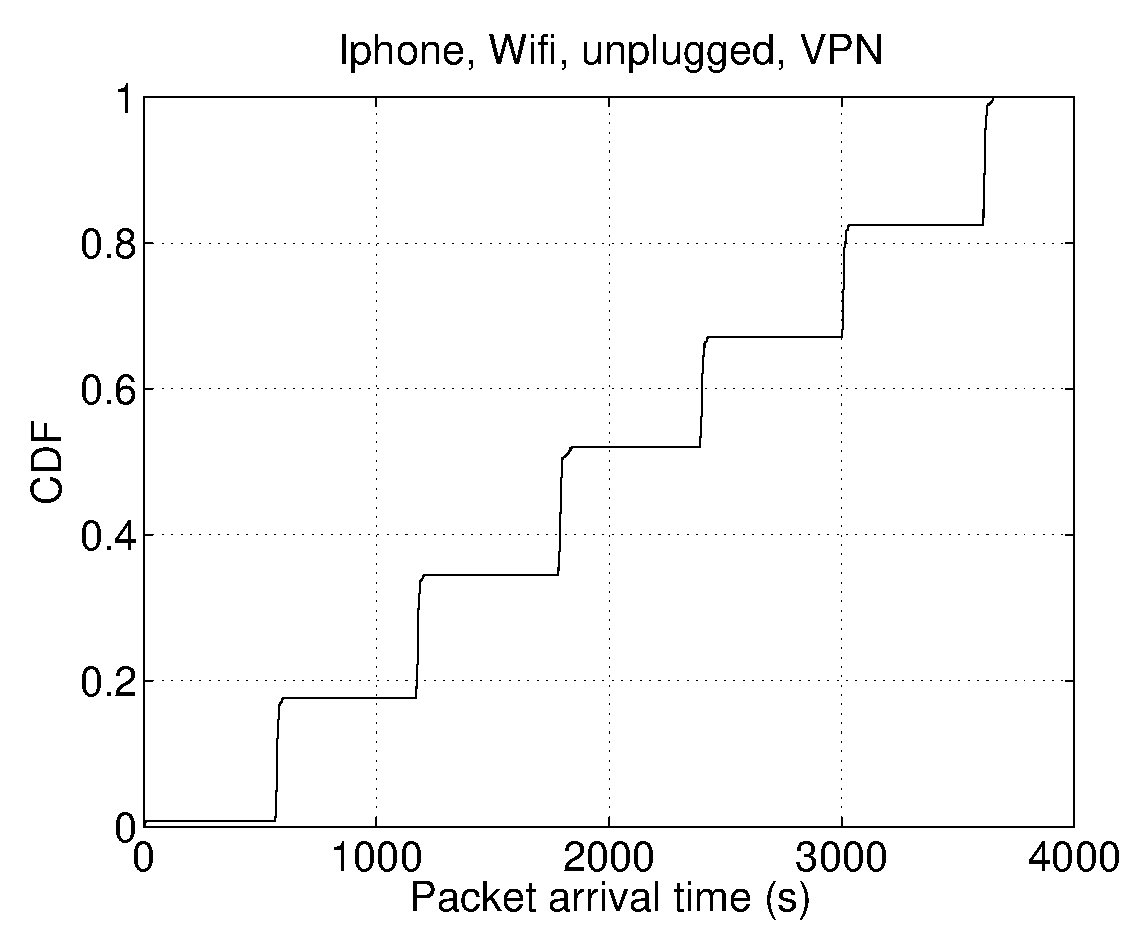
\includegraphics[width=0.8\linewidth]{../../code/pushNotification/Fig/bw_iphone_wifi_unplug_vpn_ts.eps}
  \caption{.}
  \label{fig:}
\end{figure}



%%% Local Variables: 
%%% mode: latex
%%% TeX-master: "main"
%%% End: 


\end{document}

\begin{comment}

[[1]]
  oper_sys proto service sort_order  num_flows   upanddown
1  Android   tcp    http          1 0.14873135 0.743161248
2  Android   tcp     ssl          2 0.37196187 0.243558798
3  Android   udp                  3 0.40503108 0.009736399
4  Android   tcp   other          4 0.02088602 0.002212797
5  Android other                  5 0.05338968 0.001330757

[[2]]
  oper_sys proto service sort_order  num_flows    upanddown
1      iOS   tcp    http          1 0.16066258 8.199631e-01
2      iOS   tcp     ssl          2 0.37646863 1.730939e-01
3      iOS   udp                  3 0.42336602 4.962026e-03
4      iOS   tcp   other          4 0.01130392 1.887129e-03
5      iOS other                  5 0.02819885 9.384894e-05

Traffic Share per Technology in bytes
[[1]]
  proto service sort_order orig_ip_bytes resp_ip_bytes    upanddown  num_flows upanddown_med
1   tcp    http          1  2.037205e-02  8.148594e-01 8.352315e-01 0.16903049  8.127815e-01
2   tcp     ssl          2  6.684516e-02  9.142296e-02 1.582681e-01 0.38176865  1.790630e-01
3   udp                  3  1.138886e-03  3.728491e-03 4.867377e-03 0.41419786  5.656573e-03
4   tcp   other          4  4.376426e-04  1.112469e-03 1.550112e-03 0.01375129  1.247389e-03
5 other                  5  7.908798e-05  3.840691e-06 8.292867e-05 0.02125172  8.737062e-05

[[2]]
  proto service sort_order orig_ip_bytes resp_ip_bytes   upanddown  num_flows upanddown_med
1   tcp    http          1   0.022709343  0.5387596448 0.561468988 0.13029002  0.4819883289
2   tcp     ssl          2   0.088185532  0.3261125974 0.414298130 0.36132171  0.4080785193
3   udp                  3   0.004677570  0.0121104795 0.016788049 0.41568438  0.0200971765
4   tcp   other          4   0.001868316  0.0024866839 0.004355000 0.01943862  0.0025214824
5 other                  5   0.002696138  0.0003936954 0.003089833 0.07326527  0.0002920705

\end{comment}
